
\documentclass[11pt]{article}
\usepackage[utf8]{inputenc}
\usepackage[T1]{fontenc}
\usepackage{geometry}
\usepackage{graphicx}
\usepackage{booktabs}
\usepackage{longtable}
\usepackage{array}
\usepackage{float}
\usepackage{pdflscape}
\usepackage{hyperref}
\usepackage{caption}
\usepackage{listings}
\usepackage{xcolor}
\geometry{margin=1in}
\hypersetup{colorlinks=true, linkcolor=blue, urlcolor=blue}
\lstset{
  basicstyle=\ttfamily\scriptsize,
  breaklines=true,
  columns=fullflexible,
  frame=single,
  keepspaces=true
}

\title{Sound of Culture\\Exploratory Report on the Country-Only Chords Dataset}
\author{Automated analytical note built from Stata outputs}
\date{\today}

\begin{document}
\maketitle
\tableofcontents
\clearpage

\section{Purpose of the report}
This report documents the exploratory descriptive analysis of
\path{Sound_of_Culture_Country_CountryOnly_Chords_Final_2026_04_08.dta}.
The goal is threefold: first, to clarify exactly why the analytical sample was
restricted to songs released between 1946 and 2026 and tagged as \texttt{country};
second, to read the temporal, stylistic, geographic and generational patterns in a
way that is statistically disciplined rather than purely visual; third, to leave a
fully reproducible paper trail by packaging the Stata do-file, all tables, all
figures, and the exact Stata code used for each plotted object.

The broad 1946+ sample contains 41,023 observations, but only
65.9\% of them, i.e. 27,042 songs, are
explicitly tagged as \texttt{country} by Ultimate Guitar. This is why the broad-sample
genre diagnostic is kept in the report, while the main inferential reading is based on
the stricter country-song sample.

\section{How the analysis was designed and how to read it}
The logic of the analysis is intentionally sequential.

\begin{enumerate}
\item The do-file first relabels the dataset and builds analytical variables such as release decade, artist generation, upload-release gap, and grouped first chords.
\item It then creates three nested samples: the full dataset, the 1946+ sample, and the main country-only sample used for inference.
\item It exports descriptive tables and figures for temporal trends, genre diagnostics, chord usage, geography and generations.
\item It finally estimates significance checks. For temporal plots the report uses robust linear trend regressions. For regional and generational contrasts it uses robust regressions with group dummies followed by omnibus \texttt{testparm} tests. For decade-level genre and chord share figures it uses decade-level trend regressions, which are lower-power because they rely on only nine decade points.
\end{enumerate}

The significance tests help decide whether a visible difference is plausibly systematic. They do not by themselves imply causality. With this sample size, tiny differences can be statistically significant, so the report always pairs p-values with effect size and substantive interpretation.

\begin{table}[H]
\centering
\caption{Main country-only analytical sample}
\label{tab:sample}
\begin{tabular}{lc}
\toprule
Metric & Value \\
\midrule
Analysis window & 1946--2026 \\
Country-song observations & 27,042 \\
Unique artists & 810 \\
Unique artist-song pairs & 26,995 \\
Mean age at release & 42.77 \\
Mean upload-release gap & 16.38 \\
Mean complexity & 0.107 \\
Mean repetition & 0.909 \\
Mean playability & 0.893 \\
Billboard year-end share & 4.4\% \\
\bottomrule
\end{tabular}
\end{table}

\begin{table}[H]
\centering
\caption{Coverage of key variables}
\label{tab:coverage}
\begin{tabular}{lc}
\toprule
Variable & Non-missing share \\
\midrule
release\_year & 93.4\% \\
birth\_year & 97.1\% \\
genre & 94.6\% \\
BPM & 13.9\% \\
Complexity & 98.3\% \\
Repetition & 98.3\% \\
Playability & 98.3\% \\
\bottomrule
\end{tabular}
\end{table}


\section{Structure of the Stata do-file}
The Stata file \texttt{eda\_country\_only\_chords\_2026\_04\_08.do} is organized in nine blocks.

\begin{enumerate}
\item Full relabeling of original song-level and artist-level variables.
\item Minimal cleaning and creation of derived variables such as generation and first-chord groups.
\item Overview and coverage tables for the full sample, the 1946+ sample, and the main country-only sample.
\item Temporal tables and annual trend figures for the country-only sample.
\item Genre diagnostics on the broad artist-based sample and chord-style figures on the country-only sample.
\item Geographic summaries and region-level figures.
\item Generational summaries and generation-level figures.
\item Export of an analysis-ready extract.
\item Significance tests for temporal trends and group differences.
\end{enumerate}

\section{Main descriptive and inferential findings}


\subsection{Figure 1. Annual song counts in the country-only sample}
\begin{figure}[H]
\centering
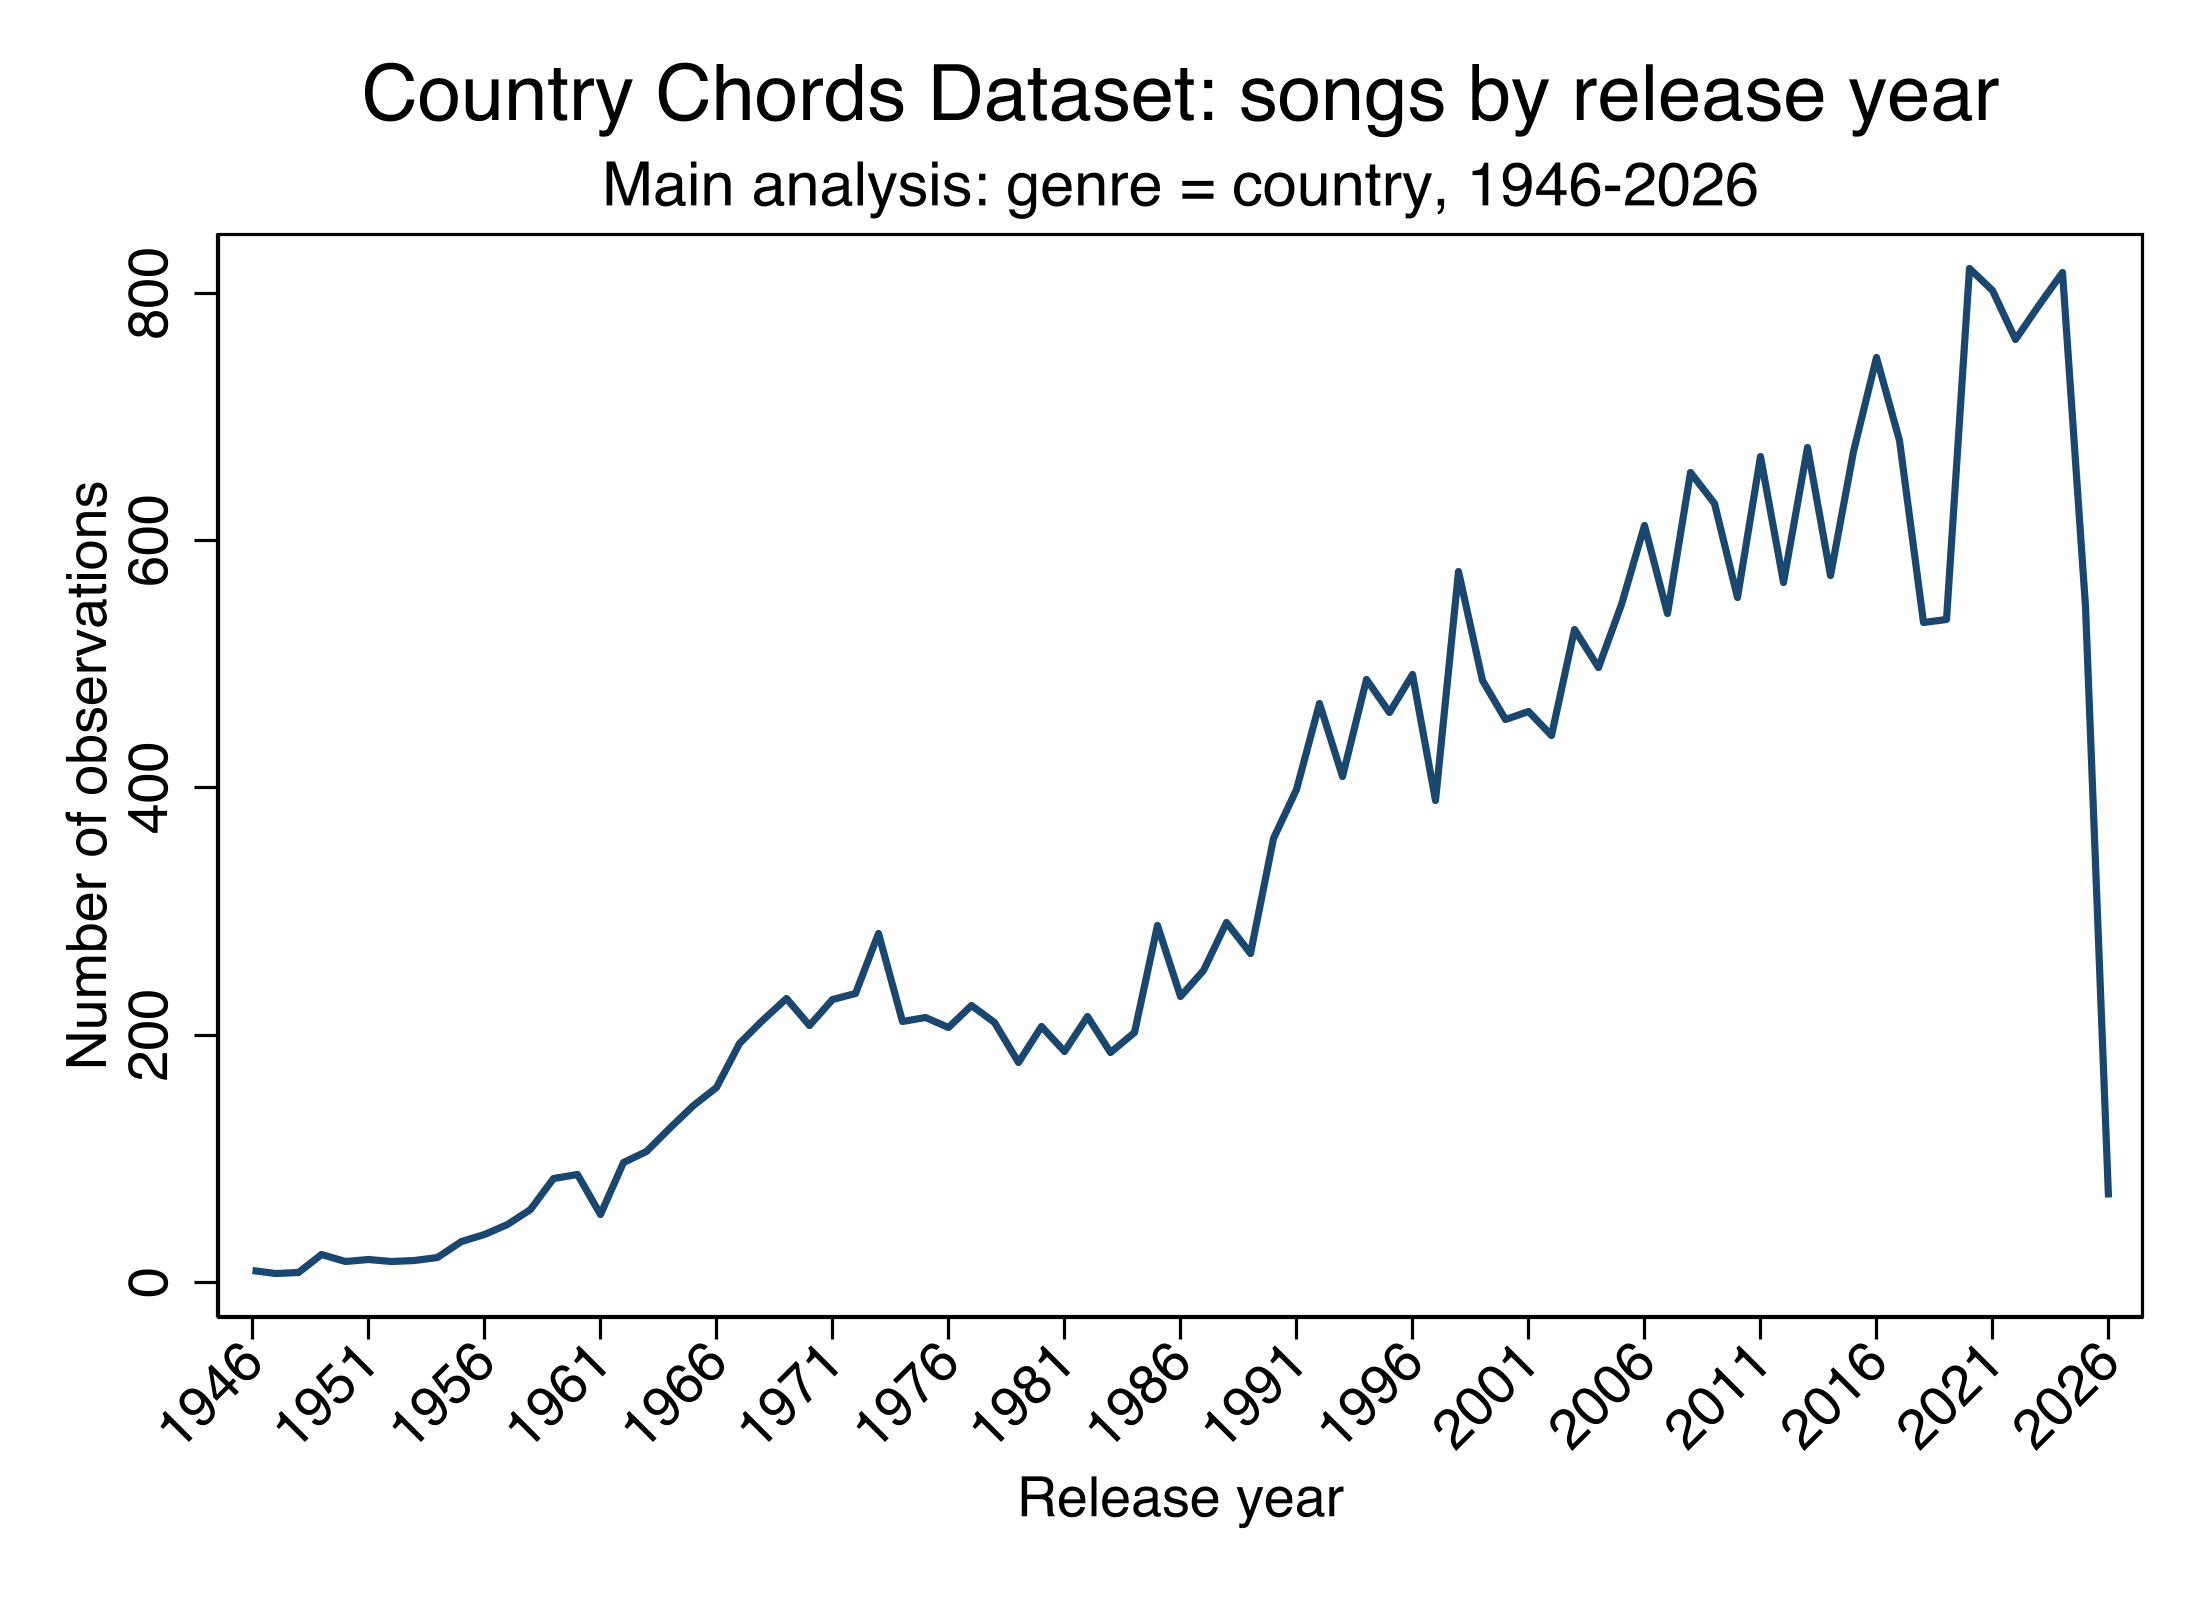
\includegraphics[width=0.92\textwidth]{analysis_outputs/graphs/01_count_songs_by_release_year.png}
\caption{Figure 1. Annual song counts in the country-only sample}
\label{fig:song_count}
\end{figure}
The number of country-tagged tabs rises strongly over time. The annual count trend is positive and statistically significant: 9.396 additional songs per year, or 93.958 per decade, with p-value $<0.001$. This figure should be read as a coverage and visibility graph rather than as a direct measure of production, because it reflects tab availability on Ultimate Guitar.

\paragraph{Stata code used for the figure.}
\begin{lstlisting}
twoway ///
    (line n_tabs release_year, lcolor(navy) lwidth(medthick)), ///
    title("Country Chords Dataset: songs by release year") ///
    subtitle("Main analysis: genre = country, `analysis_start_year'-`analysis_end_year'") ///
    xtitle("Release year") ytitle("Number of observations") ///
    xlabel(`analysis_start_year'(5)`analysis_end_year', angle(45)) ///
    xscale(range(`analysis_start_year' `analysis_end_year'))
graph export "`graph_dir'/01_count_songs_by_release_year.png", replace width(2200)
\end{lstlisting}



\subsection{Figure 2. Average BPM by release year}
\begin{figure}[H]
\centering
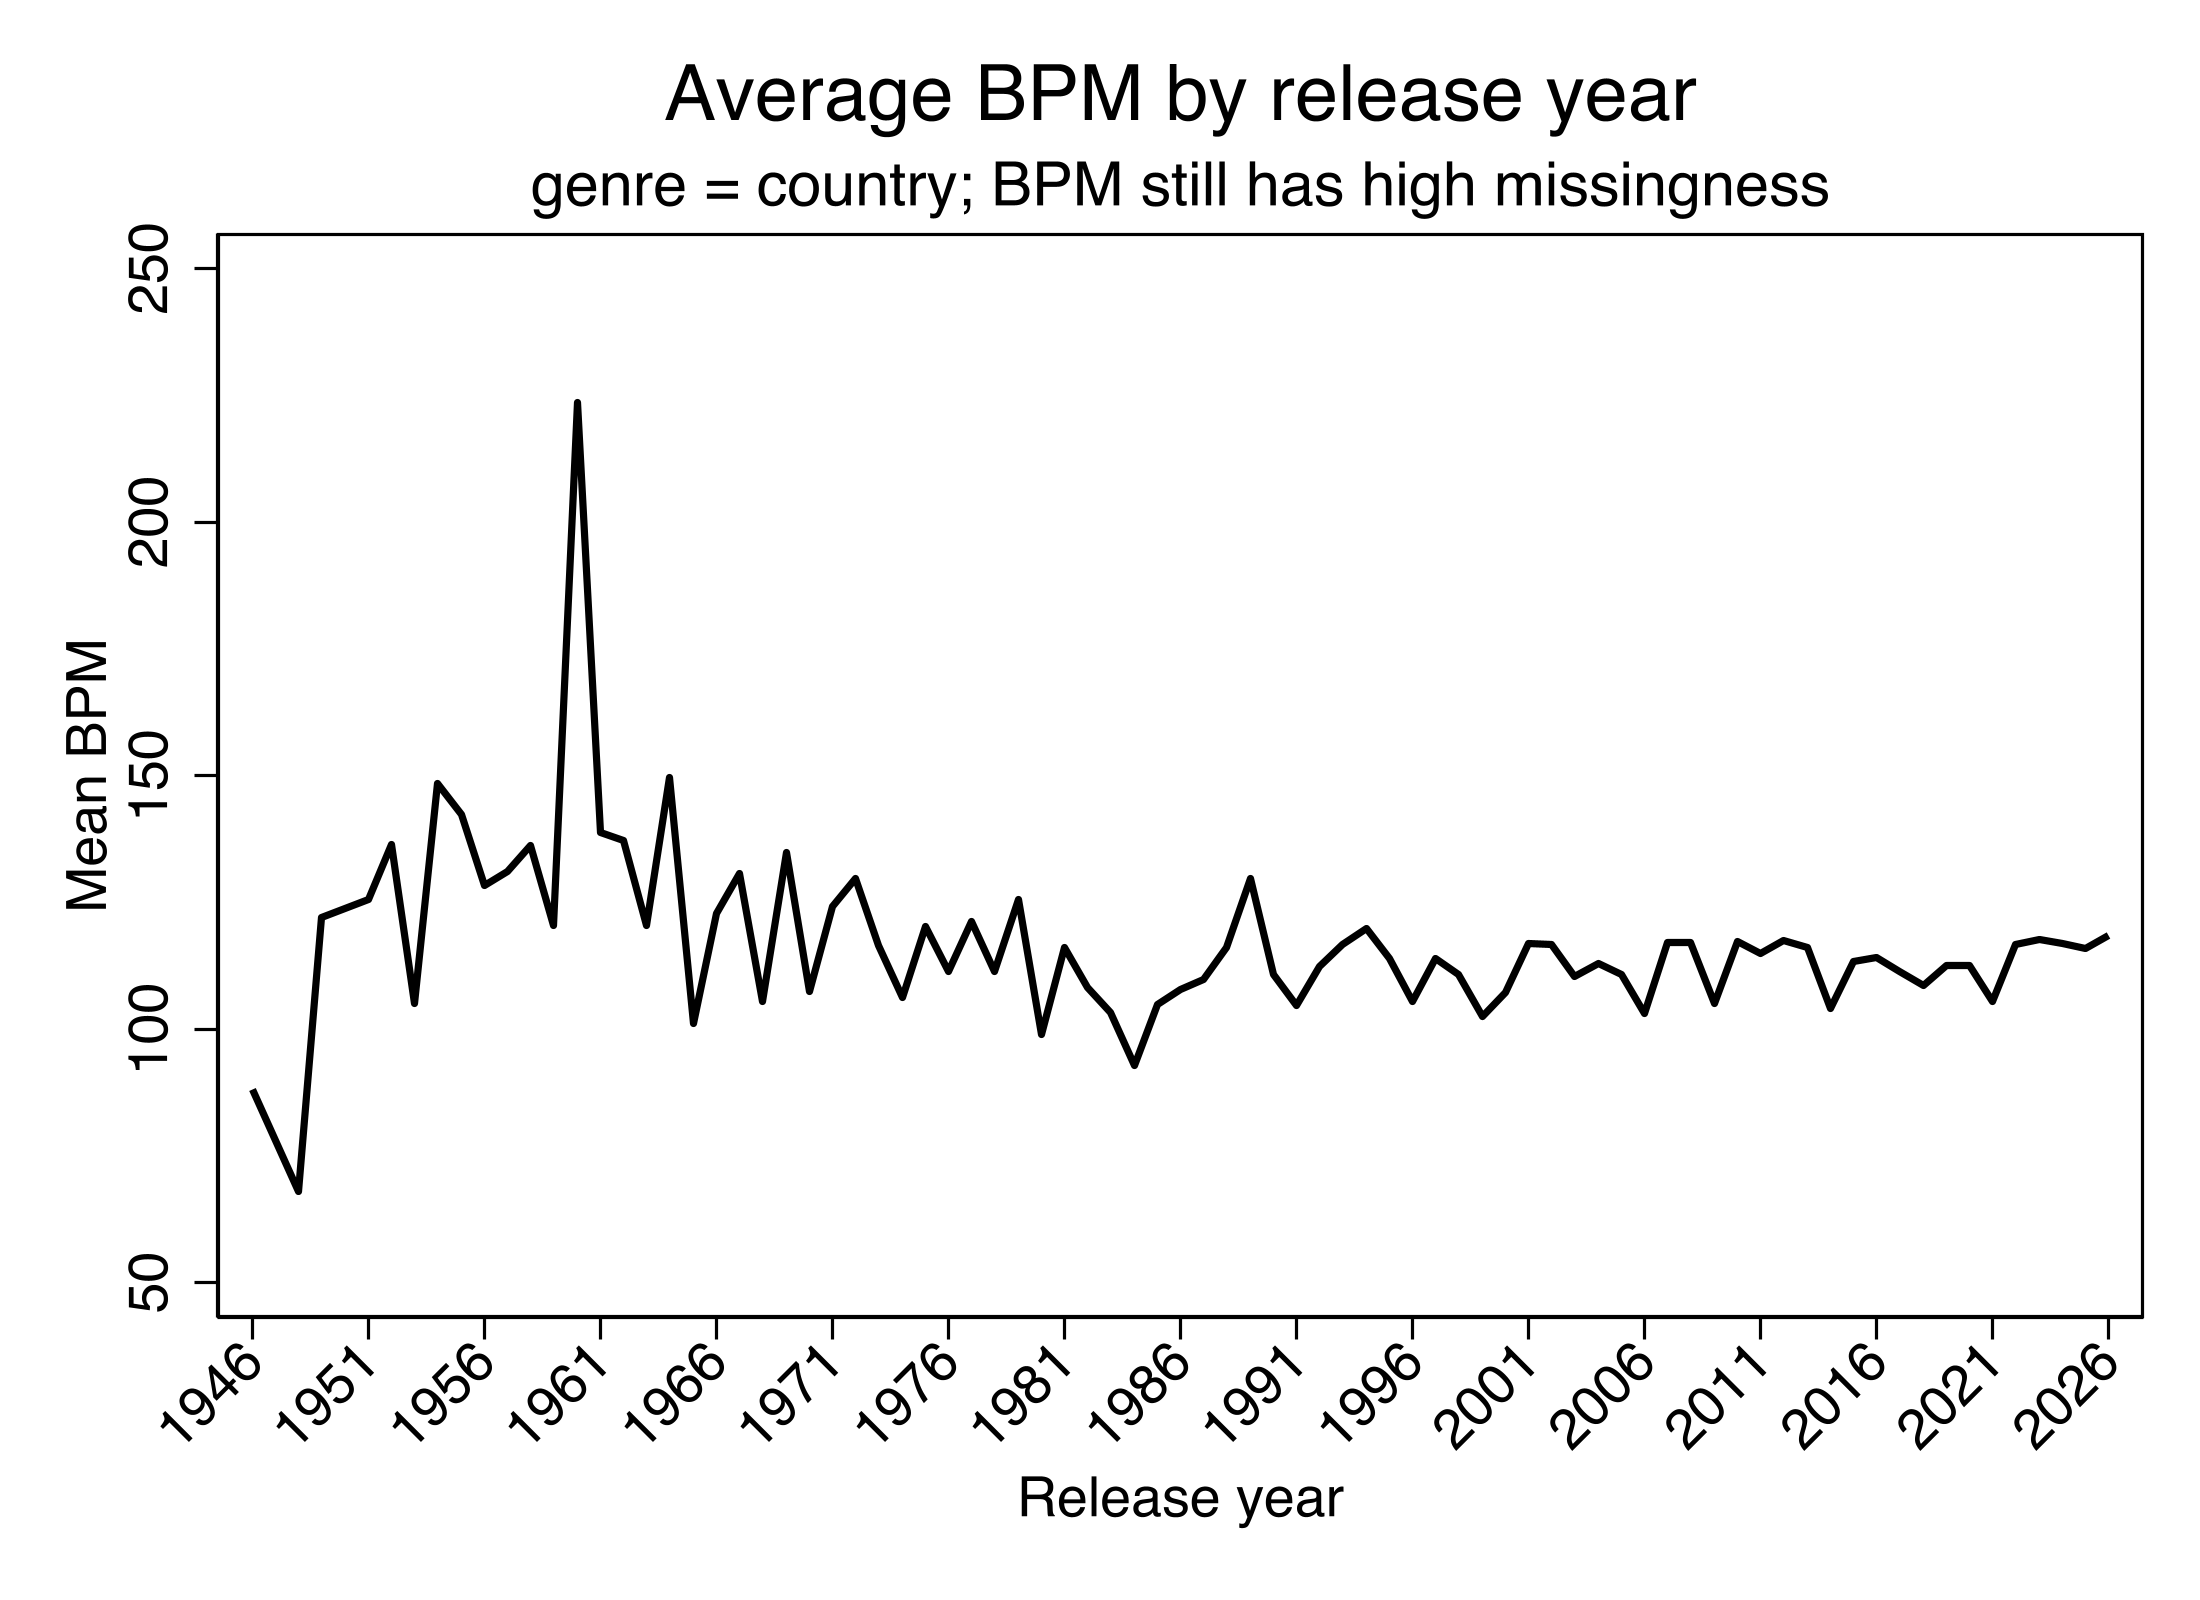
\includegraphics[width=0.92\textwidth]{analysis_outputs/graphs/02_bpm_by_release_year.png}
\caption{Figure 2. Average BPM by release year}
\label{fig:bpm}
\end{figure}
BPM has much weaker evidence of secular change. The estimated slope is -0.863 BPM per decade with p-value 0.060. Because BPM is observed for only a minority of songs, the figure is informative but should be treated as suggestive rather than central.

\paragraph{Stata code used for the figure.}
\begin{lstlisting}
twoway ///
    (line bpm release_year, lcolor(black) lwidth(medthick)), ///
    title("Average BPM by release year") ///
    subtitle("genre = country; BPM still has high missingness") ///
    xtitle("Release year") ytitle("Mean BPM") ///
    xlabel(`analysis_start_year'(5)`analysis_end_year', angle(45)) ///
    xscale(range(`analysis_start_year' `analysis_end_year'))
graph export "`graph_dir'/02_bpm_by_release_year.png", replace width(2200)
\end{lstlisting}



\subsection{Figure 3. Mechanics and difficulty indices over time}
\begin{figure}[H]
\centering
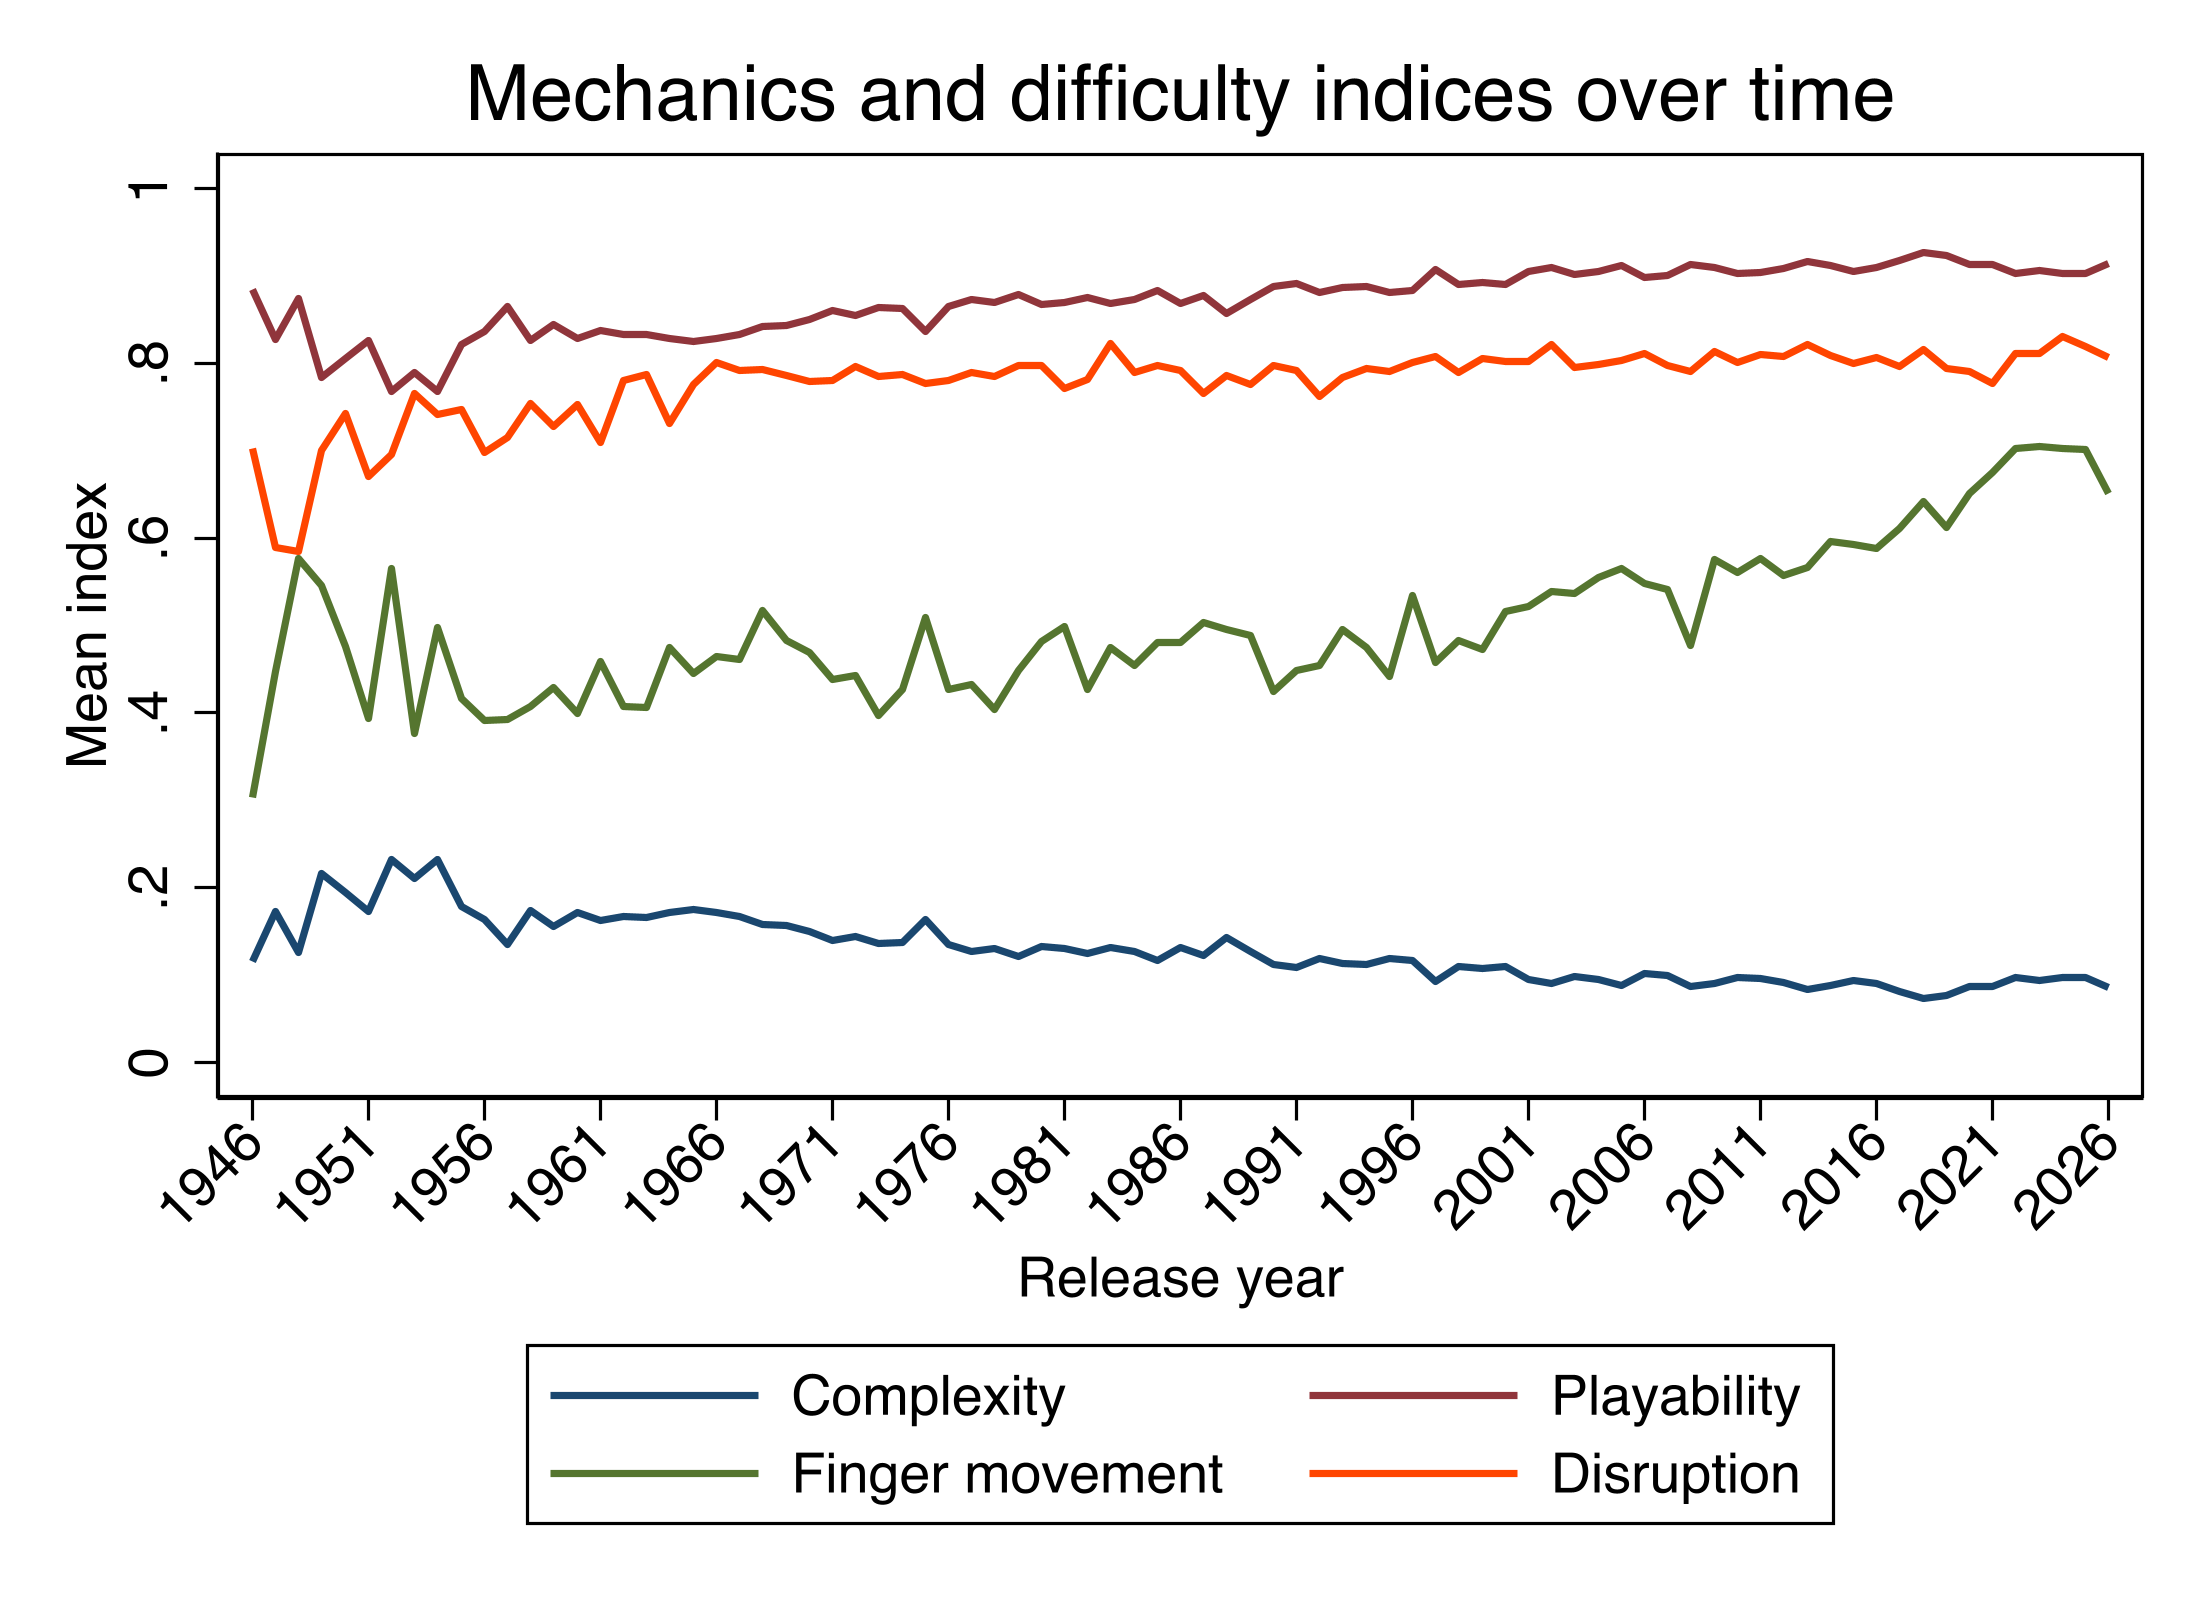
\includegraphics[width=0.92\textwidth]{analysis_outputs/graphs/03_indices_mechanics_by_release_year.png}
\caption{Figure 3. Mechanics and difficulty indices over time}
\label{fig:mechanics}
\end{figure}
Mechanically, the repertoire becomes easier and more standardized. Complexity decreases significantly ($<0.001$), playability rises in almost mirror-image form ($<0.001$), finger movement increases modestly but significantly, and disruption also increases slightly. The joint reading is that modern country songs use easier-to-play chord systems but with somewhat more movement across the sequence.

\paragraph{Stata code used for the figure.}
\begin{lstlisting}
twoway ///
    (line complexity release_year, lcolor(navy) lwidth(medthick)) ///
    (line playability release_year, lcolor(maroon) lwidth(medthick)) ///
    (line finger_movement release_year, lcolor(forest_green) lwidth(medthick)) ///
    (line disruption release_year, lcolor(orange_red) lwidth(medthick)), ///
    title("Mechanics and difficulty indices over time") ///
    xtitle("Release year") ytitle("Mean index") ///
    xlabel(`analysis_start_year'(5)`analysis_end_year', angle(45)) ///
    xscale(range(`analysis_start_year' `analysis_end_year')) ///
    legend(order(1 "Complexity" 2 "Playability" 3 "Finger movement" 4 "Disruption"))
graph export "`graph_dir'/03_indices_mechanics_by_release_year.png", replace width(2200)
\end{lstlisting}



\subsection{Figure 4. Rhythm and form indices over time}
\begin{figure}[H]
\centering
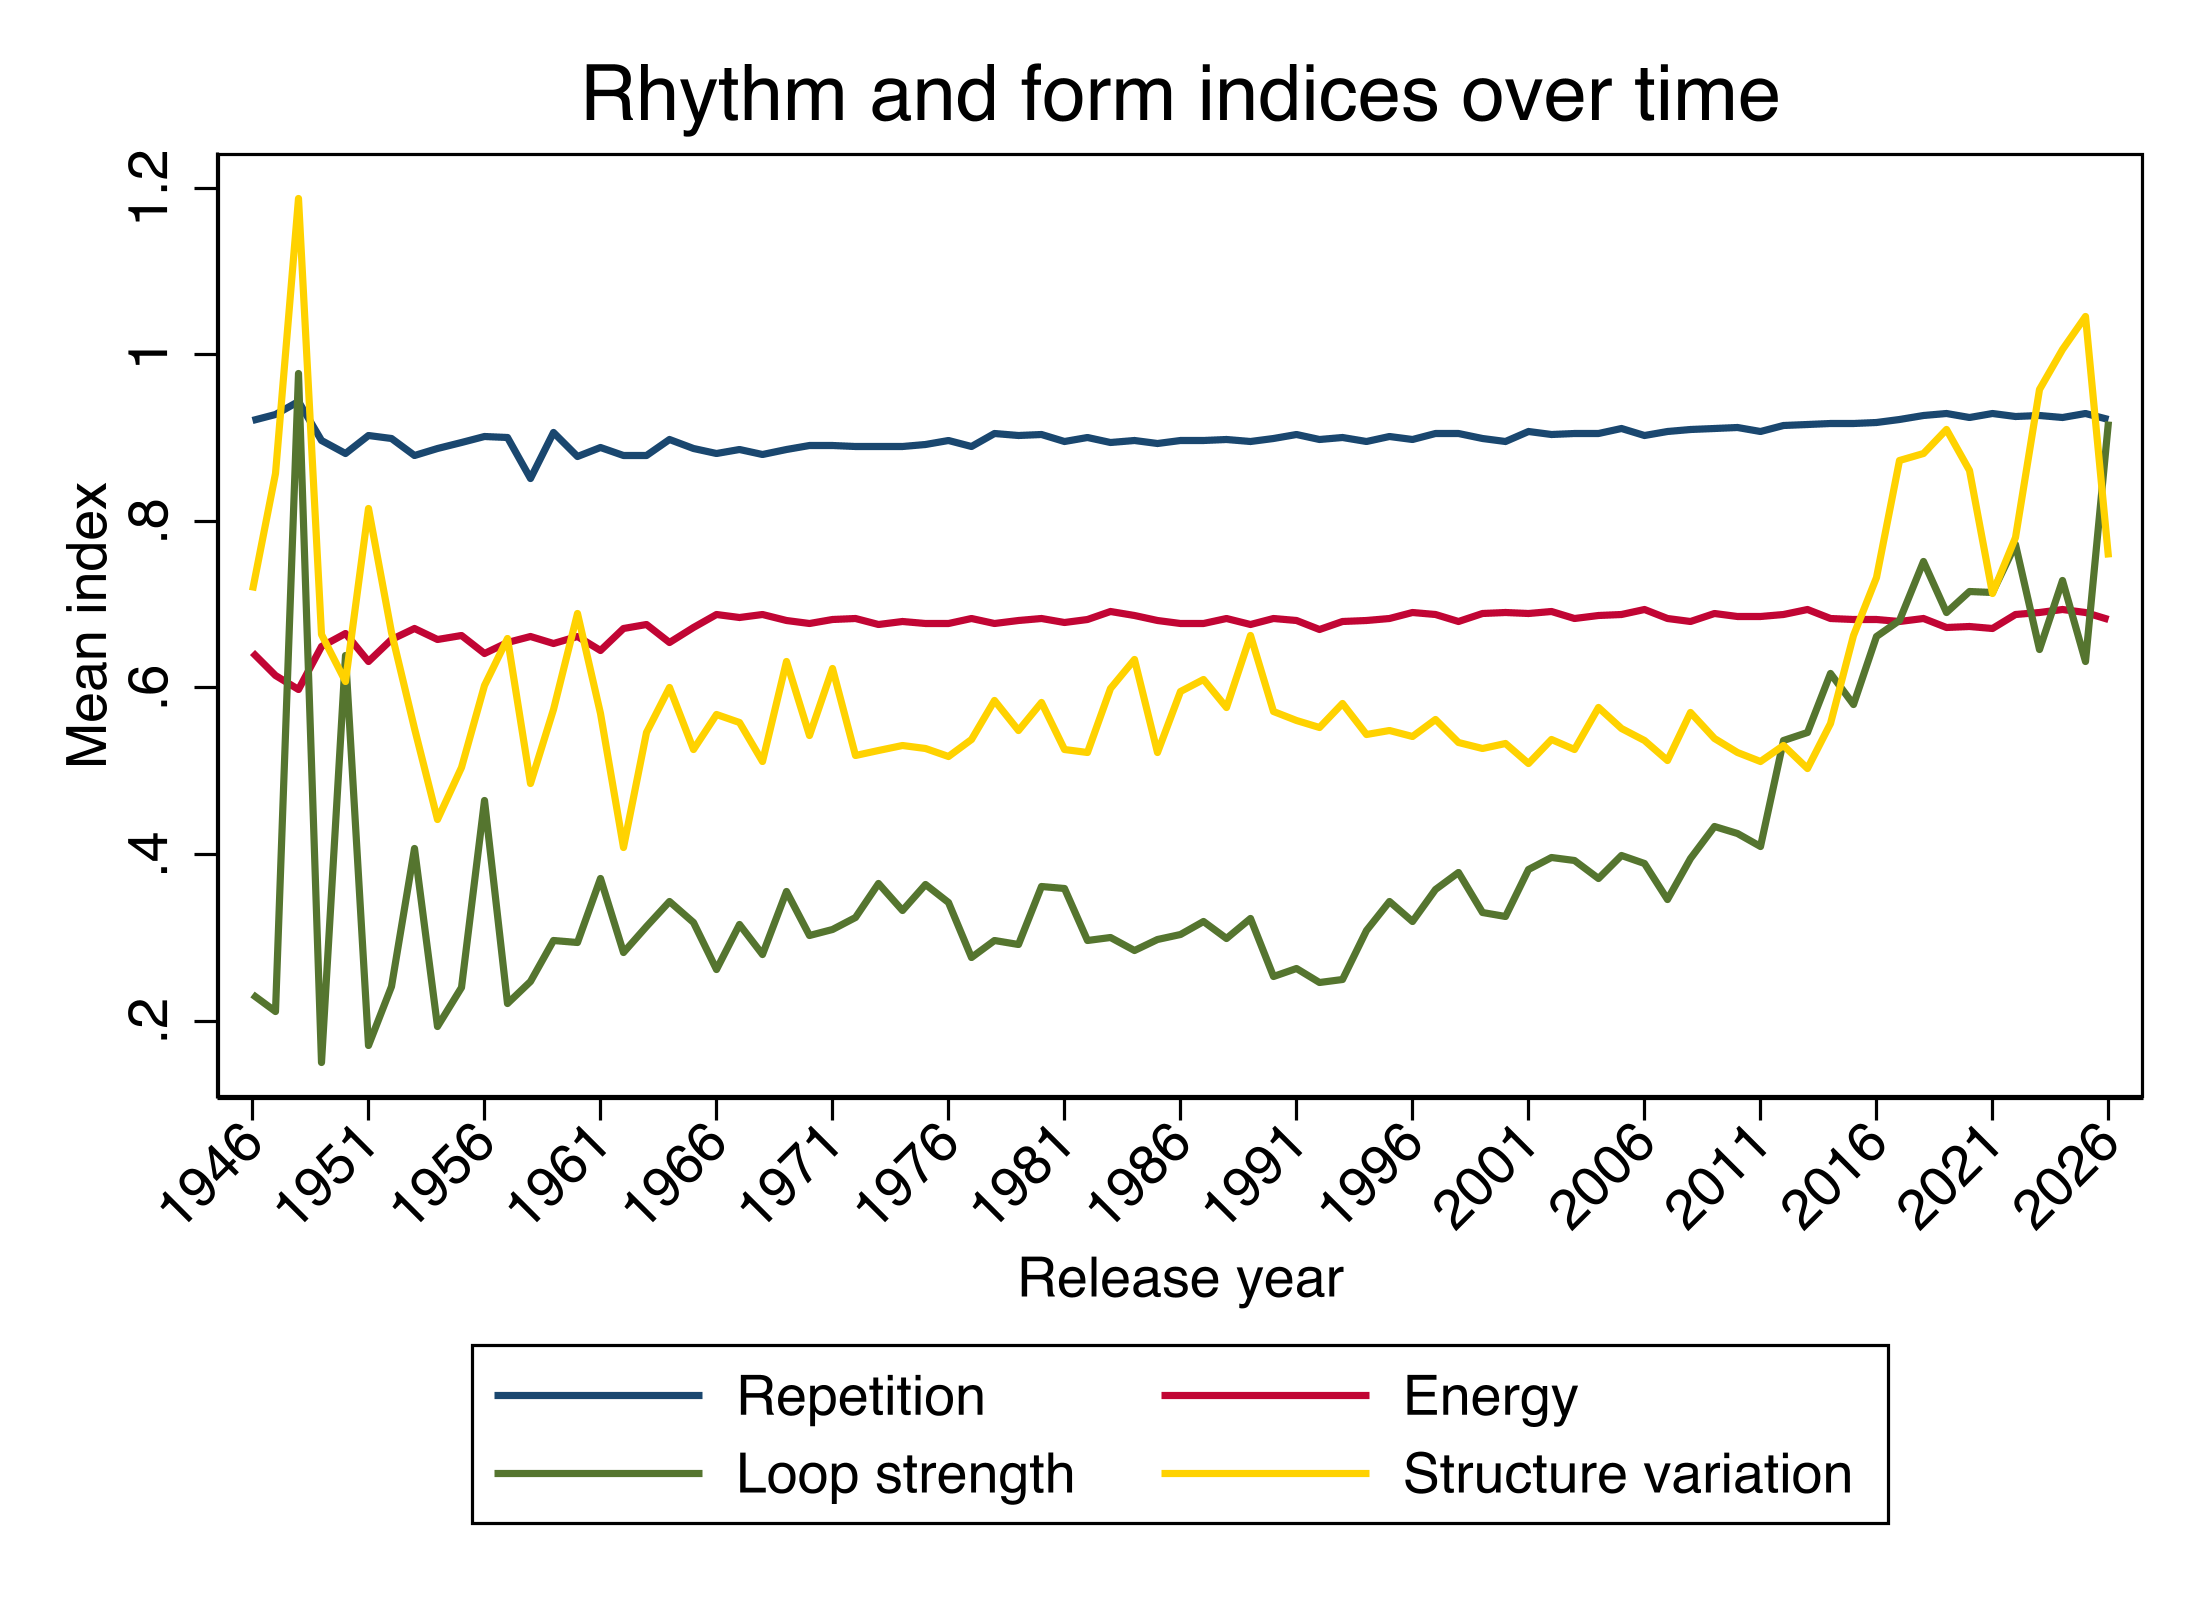
\includegraphics[width=0.92\textwidth]{analysis_outputs/graphs/04_indices_rhythm_form_by_release_year.png}
\caption{Figure 4. Rhythm and form indices over time}
\label{fig:rhythm}
\end{figure}
Repetition, loop strength and structure variation all trend upward and all three slopes are statistically significant at conventional levels. Energy also increases, but the effect is small in magnitude. This indicates a repertoire that becomes more loop-friendly and formally segmented over time, even while remaining harmonically accessible.

\paragraph{Stata code used for the figure.}
\begin{lstlisting}
twoway ///
    (line repetition release_year, lcolor(navy) lwidth(medthick)) ///
    (line energy release_year, lcolor(cranberry) lwidth(medthick)) ///
    (line loop_strength release_year, lcolor(forest_green) lwidth(medthick)) ///
    (line structure_variation release_year, lcolor(gold) lwidth(medthick)), ///
    title("Rhythm and form indices over time") ///
    xtitle("Release year") ytitle("Mean index") ///
    xlabel(`analysis_start_year'(5)`analysis_end_year', angle(45)) ///
    xscale(range(`analysis_start_year' `analysis_end_year')) ///
    legend(order(1 "Repetition" 2 "Energy" 3 "Loop strength" 4 "Structure variation"))
graph export "`graph_dir'/04_indices_rhythm_form_by_release_year.png", replace width(2200)
\end{lstlisting}



\subsection{Figure 5. Harmony indices over time}
\begin{figure}[H]
\centering
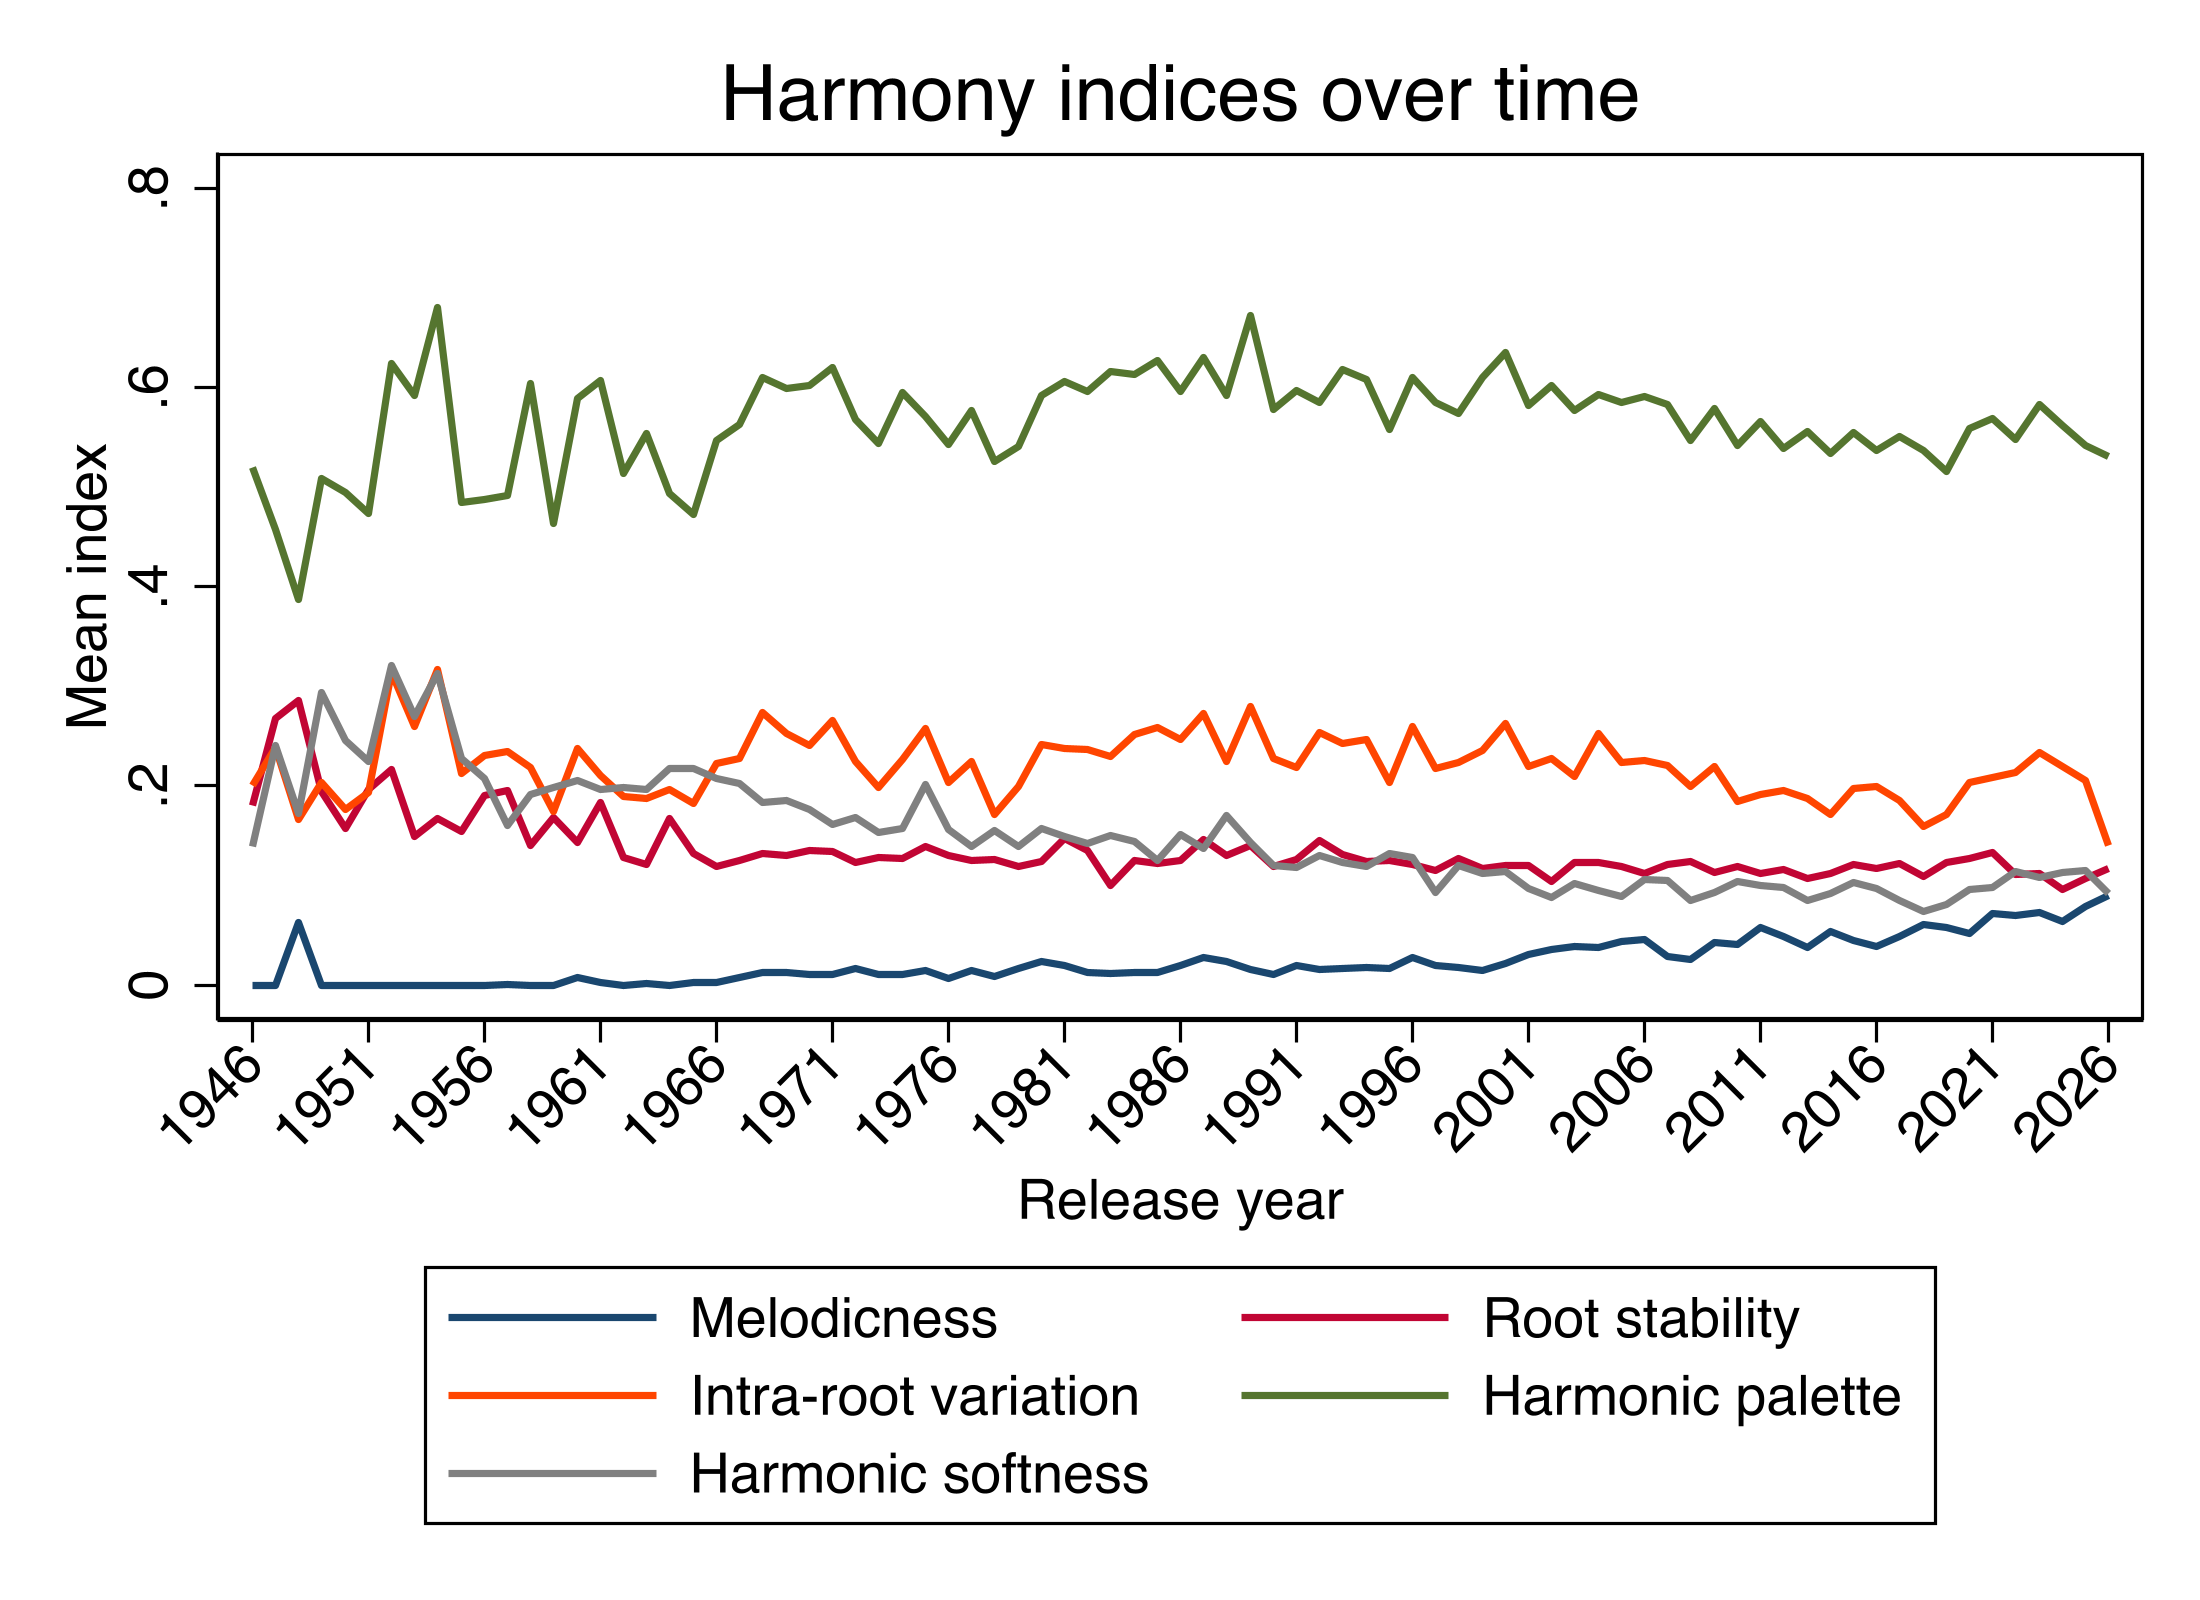
\includegraphics[width=0.92\textwidth]{analysis_outputs/graphs/05_indices_harmony_by_release_year.png}
\caption{Figure 5. Harmony indices over time}
\label{fig:harmony}
\end{figure}
The harmony panel shows a mixed but coherent transition. Melodicness rises significantly, while root stability, intra-root variation, harmonic palette and harmonic softness all decline. Substantively, this suggests that the modern country sample relies on fewer distinct harmonic resources and less soft-chord coloring, even as consonant melodic motion becomes more common.

\paragraph{Stata code used for the figure.}
\begin{lstlisting}
twoway ///
    (line melodicness release_year, lcolor(navy) lwidth(medthick)) ///
    (line root_stability release_year, lcolor(cranberry) lwidth(medthick)) ///
    (line intra_root_variation release_year, lcolor(orange_red) lwidth(medthick)) ///
    (line harmonic_palette release_year, lcolor(forest_green) lwidth(medthick)) ///
    (line harmonic_softness release_year, lcolor(gs8) lwidth(medthick)), ///
    title("Harmony indices over time") ///
    xtitle("Release year") ytitle("Mean index") ///
    xlabel(`analysis_start_year'(5)`analysis_end_year', angle(45)) ///
    xscale(range(`analysis_start_year' `analysis_end_year')) ///
    legend(order(1 "Melodicness" 2 "Root stability" 3 "Intra-root variation" ///
                 4 "Harmonic palette" 5 "Harmonic softness") cols(2))
graph export "`graph_dir'/05_indices_harmony_by_release_year.png", replace width(2200)
\end{lstlisting}



\subsection{Figure 6. Billboard prominence and upload-release gap}
\begin{figure}[H]
\centering
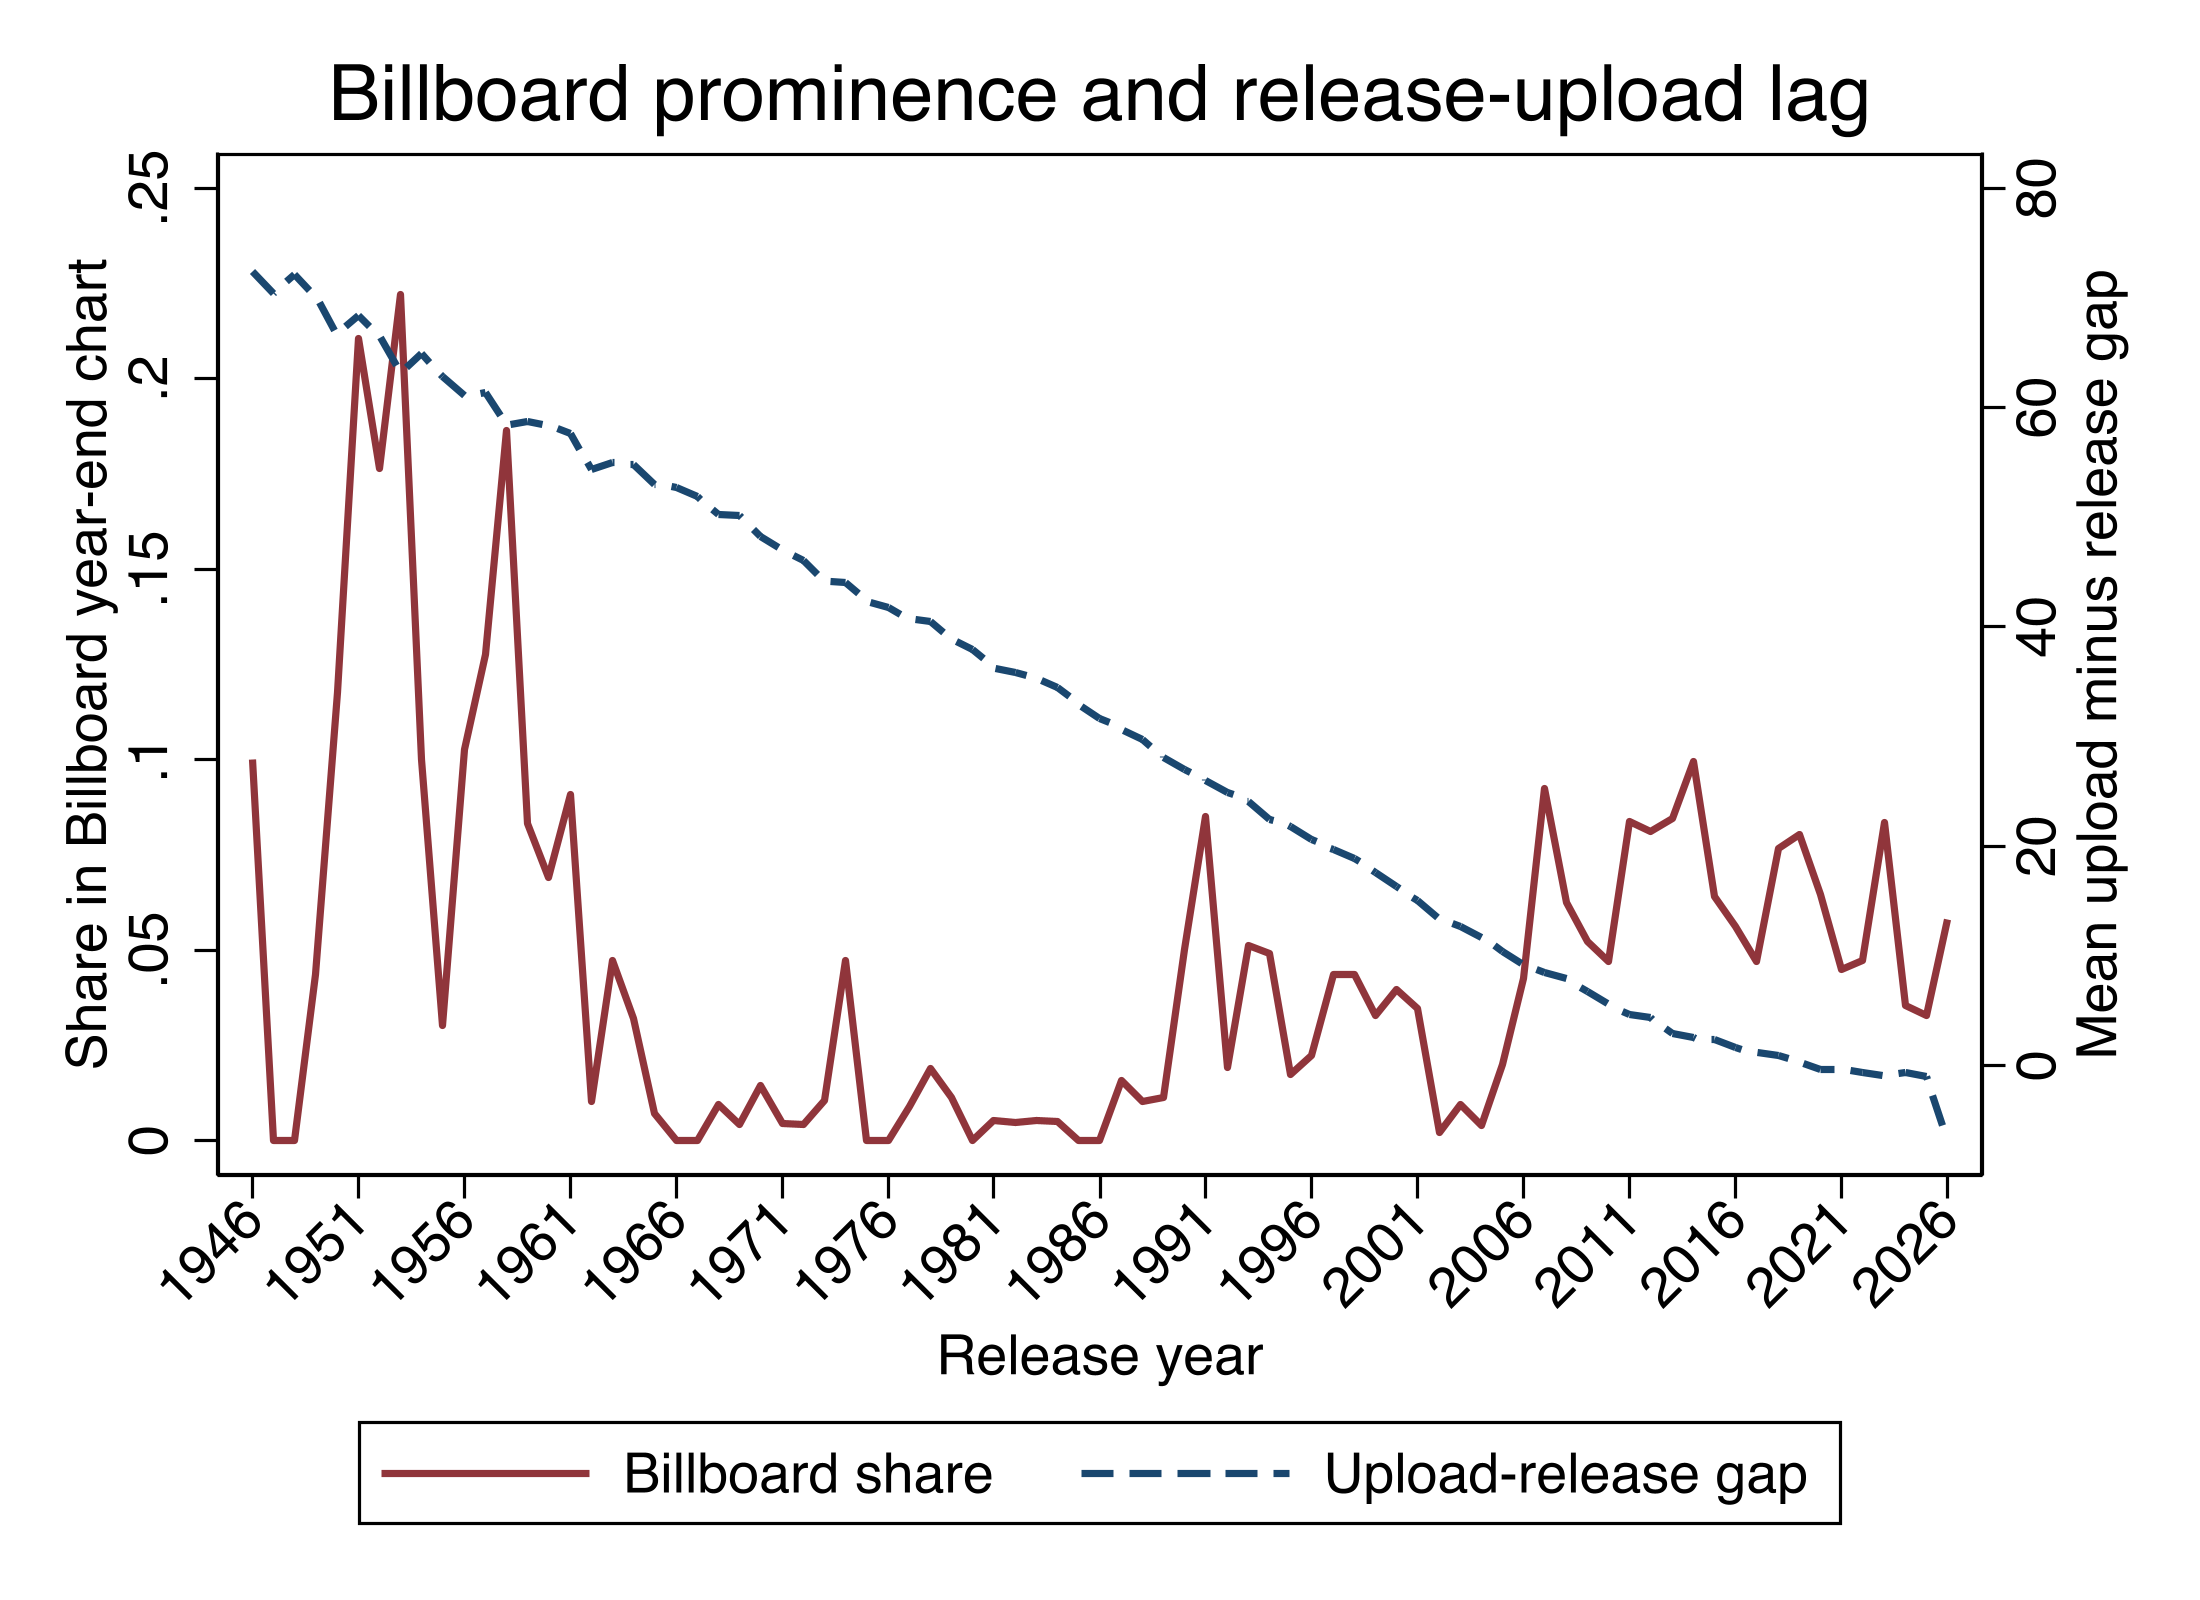
\includegraphics[width=0.92\textwidth]{analysis_outputs/graphs/06_billboard_and_release_upload_gap.png}
\caption{Figure 6. Billboard prominence and upload-release gap}
\label{fig:billboard_gap}
\end{figure}
The Billboard share increases slightly but significantly ($<0.001$), while the upload-release gap collapses mechanically and statistically ($<0.001$). The second result is especially strong and mostly reflects digital-era contemporaneity: newer songs are uploaded almost immediately relative to release.

\paragraph{Stata code used for the figure.}
\begin{lstlisting}
twoway ///
    (line share_billboard_year_end release_year, lcolor(maroon) lwidth(medthick)) ///
    (line release_upload_gap release_year, yaxis(2) lcolor(navy) lpattern(dash) lwidth(medthick)), ///
    title("Billboard prominence and release-upload lag") ///
    xtitle("Release year") ///
    ytitle("Share in Billboard year-end chart", axis(1)) ///
    ytitle("Mean upload minus release gap", axis(2)) ///
    xlabel(`analysis_start_year'(5)`analysis_end_year', angle(45)) ///
    xscale(range(`analysis_start_year' `analysis_end_year')) ///
    legend(order(1 "Billboard share" 2 "Upload-release gap") cols(2))
graph export "`graph_dir'/06_billboard_and_release_upload_gap.png", replace width(2200)
\end{lstlisting}



\subsection{Figure 7. Broad-sample genre diagnostic}
\begin{figure}[H]
\centering
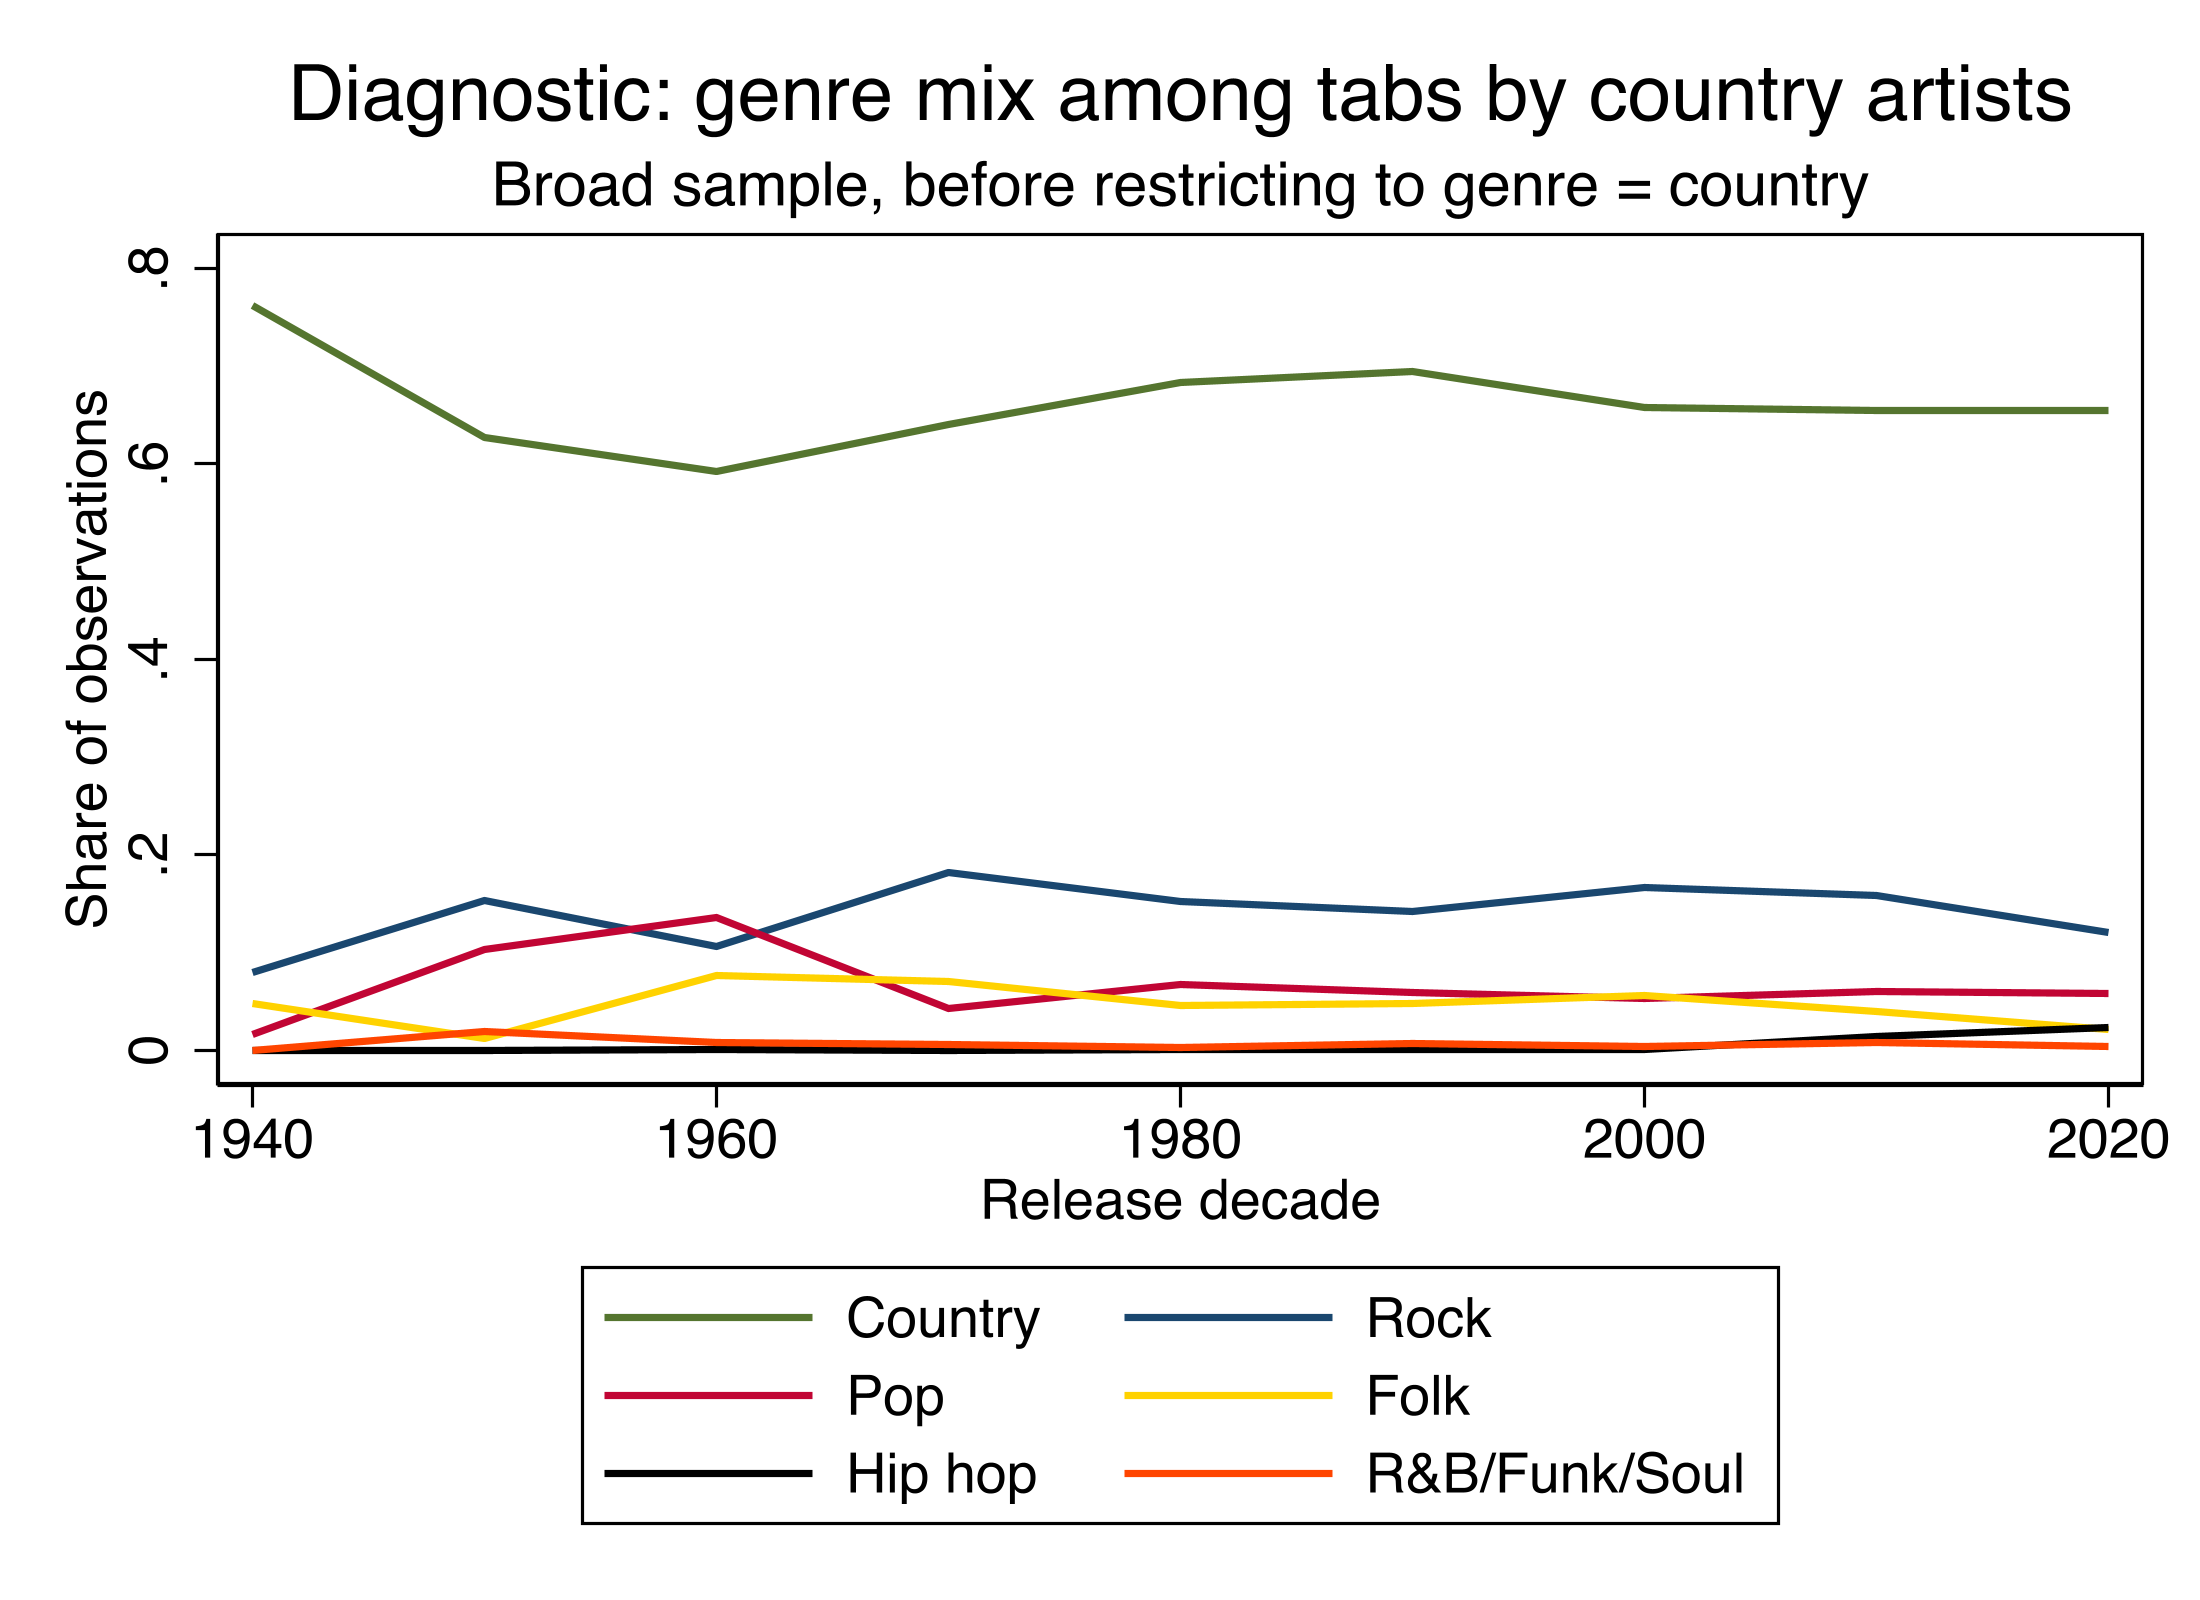
\includegraphics[width=0.92\textwidth]{analysis_outputs/graphs/07_diagnostic_genre_shares_by_release_decade_broad_sample.png}
\caption{Figure 7. Broad-sample genre diagnostic}
\label{fig:genre_diagnostic}
\end{figure}
This diagnostic explains why the report restricts the main sample. Even among country artists, the song-level metadata are not exclusively country. The broad sample retains a country share between about 59\% and 69\% by decade, while rock and pop remain substantial. The country share itself does not show a significant linear trend across decades (p-value 0.744), which means that the cross-genre contamination is persistent rather than concentrated in one period.

\paragraph{Stata code used for the figure.}
\begin{lstlisting}
twoway ///
    (line genre_country release_decade, lcolor(forest_green) lwidth(medthick)) ///
    (line genre_rock release_decade, lcolor(navy) lwidth(medthick)) ///
    (line genre_pop release_decade, lcolor(cranberry) lwidth(medthick)) ///
    (line genre_folk release_decade, lcolor(gold) lwidth(medthick)) ///
    (line genre_hiphop release_decade, lcolor(black) lwidth(medthick)) ///
    (line genre_rbsoul release_decade, lcolor(orange_red) lwidth(medthick)), ///
    title("Diagnostic: genre mix among tabs by country artists") ///
    subtitle("Broad sample, before restricting to genre = country") ///
    xtitle("Release decade") ytitle("Share of observations") ///
    legend(order(1 "Country" 2 "Rock" 3 "Pop" 4 "Folk" 5 "Hip hop" 6 "R&B/Funk/Soul") cols(2))
graph export "`graph_dir'/07_diagnostic_genre_shares_by_release_decade_broad_sample.png", replace width(2200)
\end{lstlisting}



\subsection{Figure 8. First-chord shares over release decades}
\begin{figure}[H]
\centering
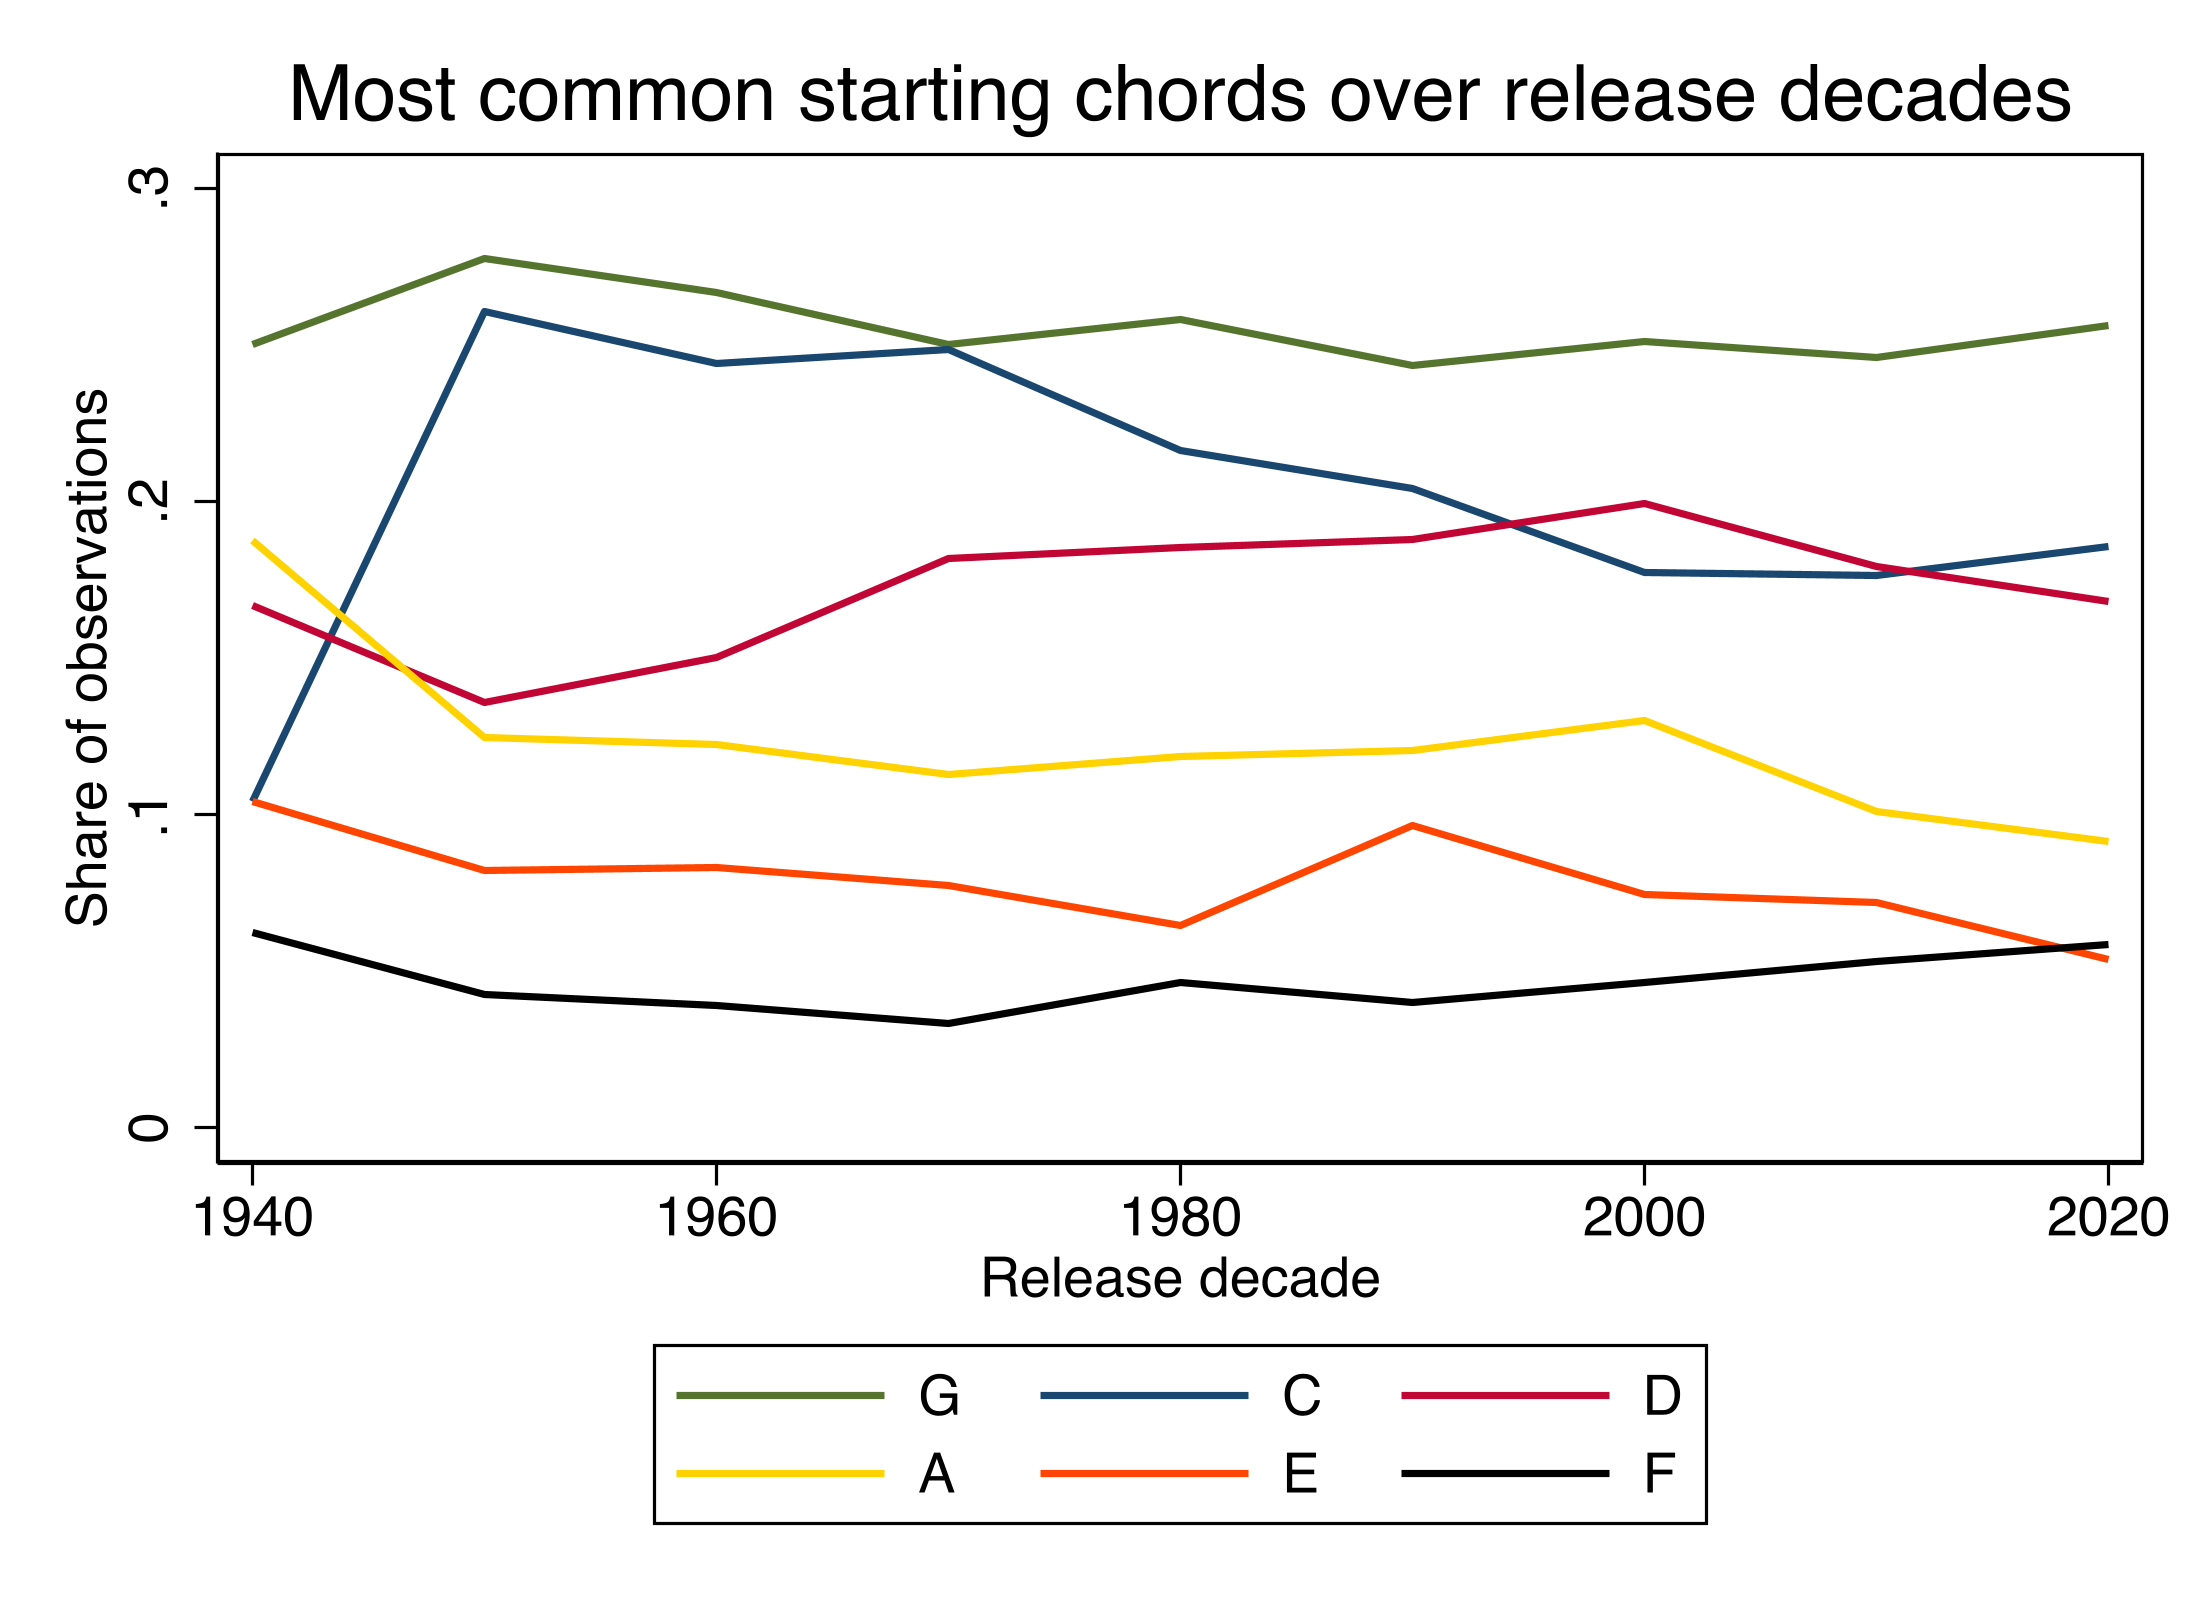
\includegraphics[width=0.92\textwidth]{analysis_outputs/graphs/08_first_chord_shares_by_release_decade.png}
\caption{Figure 8. First-chord shares over release decades}
\label{fig:first_chords}
\end{figure}
The first-chord distribution is remarkably stable. G remains dominant throughout, C and D stay broadly flat, A declines at borderline significance (p-value 0.054), and E shows a clearer negative trend (p-value 0.019). This stability reinforces the idea that the country harmonic core is persistent even as other dimensions evolve.

\paragraph{Stata code used for the figure.}
\begin{lstlisting}
twoway ///
    (line chord_g release_decade, lcolor(forest_green) lwidth(medthick)) ///
    (line chord_c release_decade, lcolor(navy) lwidth(medthick)) ///
    (line chord_d release_decade, lcolor(cranberry) lwidth(medthick)) ///
    (line chord_a release_decade, lcolor(gold) lwidth(medthick)) ///
    (line chord_e release_decade, lcolor(orange_red) lwidth(medthick)) ///
    (line chord_f release_decade, lcolor(black) lwidth(medthick)), ///
    title("Most common starting chords over release decades") ///
    xtitle("Release decade") ytitle("Share of observations") ///
    legend(order(1 "G" 2 "C" 3 "D" 4 "A" 5 "E" 6 "F") cols(3))
graph export "`graph_dir'/08_first_chord_shares_by_release_decade.png", replace width(2200)
\end{lstlisting}



\subsection{Figure 9. Geographic concentration by macro-region}
\begin{figure}[H]
\centering
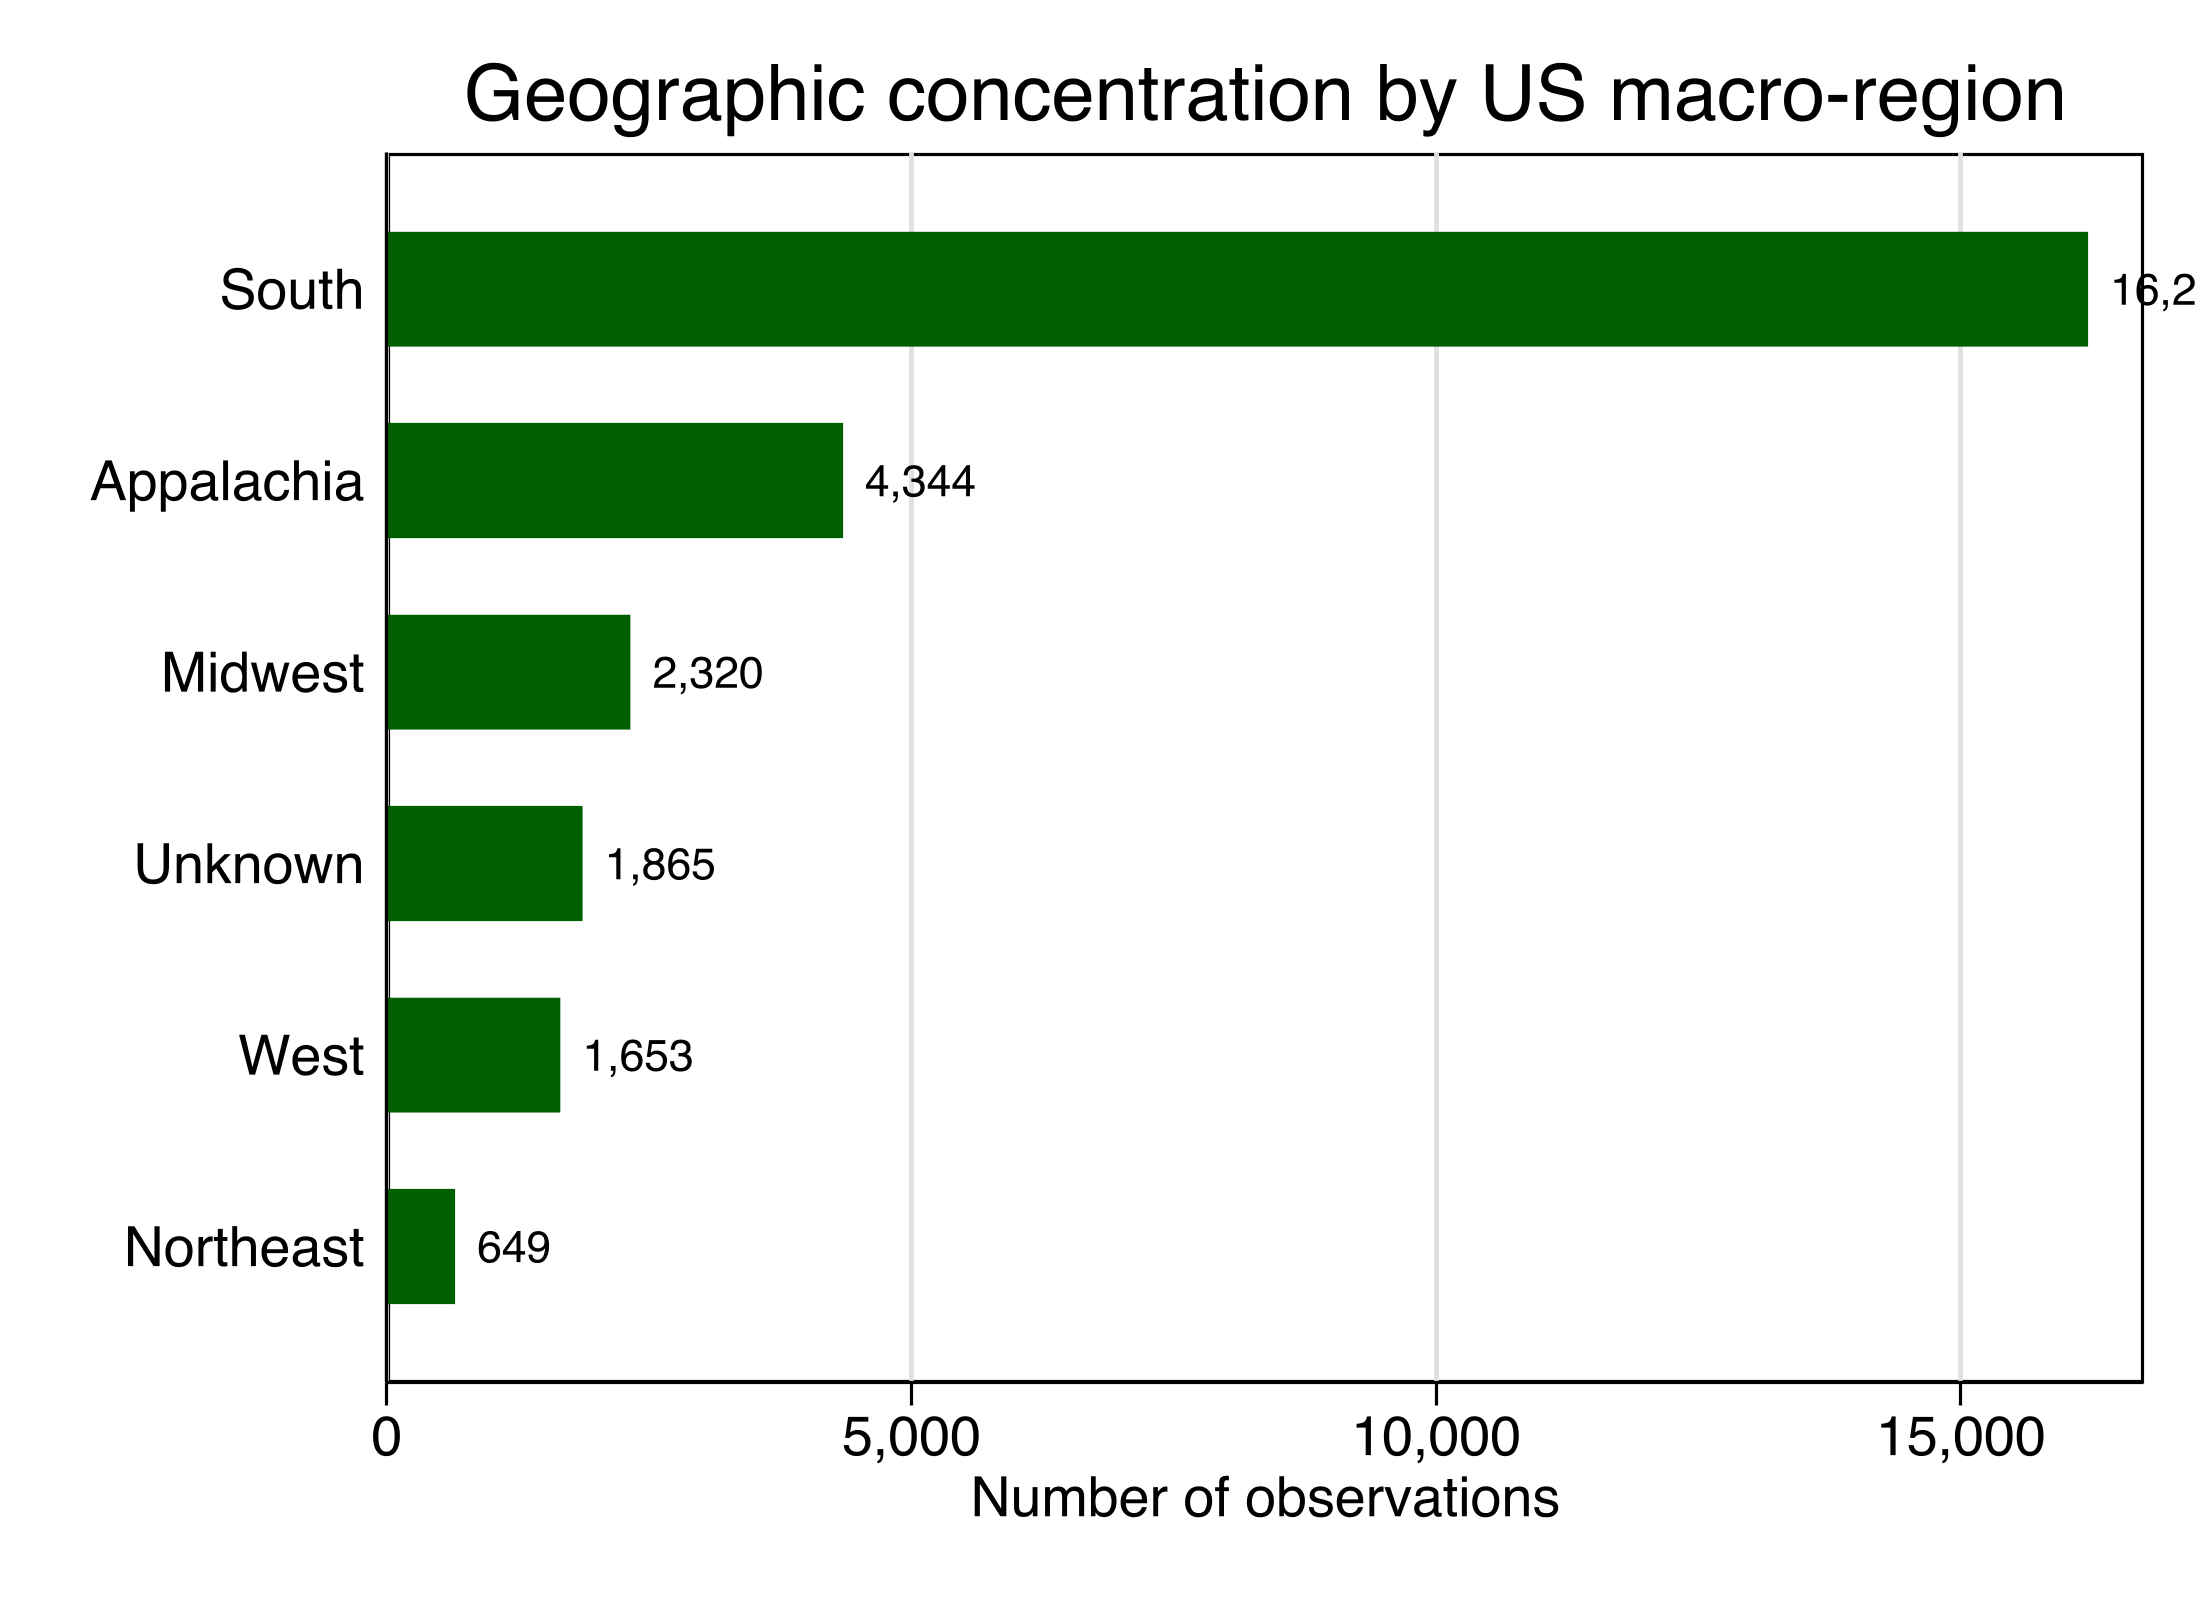
\includegraphics[width=0.92\textwidth]{analysis_outputs/graphs/09_macro_region_distribution.png}
\caption{Figure 9. Geographic concentration by macro-region}
\label{fig:geo_counts}
\end{figure}
The country-only sample is geographically concentrated. The South alone contributes 16,211 songs, about 59.9\% of the analytical sample. Appalachia is the second major cluster with 4,344 songs. At the country level, the dominant birth country is United States; at the state level the leading state is Texas. This figure is descriptive and should be interpreted together with Figure~\ref{fig:geo_indices}, where the inferential group contrasts are tested directly.

\paragraph{Stata code used for the figure.}
\begin{lstlisting}
graph hbar n_tabs, ///
    over(macro_region_clean, sort(1) descending) ///
    title("Geographic concentration by US macro-region") ///
    ytitle("Number of observations") blabel(bar, format(%9.0fc))
graph export "`graph_dir'/09_macro_region_distribution.png", replace width(2200)
\end{lstlisting}



\subsection{Figure 10. Index differences by macro-region}
\begin{figure}[H]
\centering
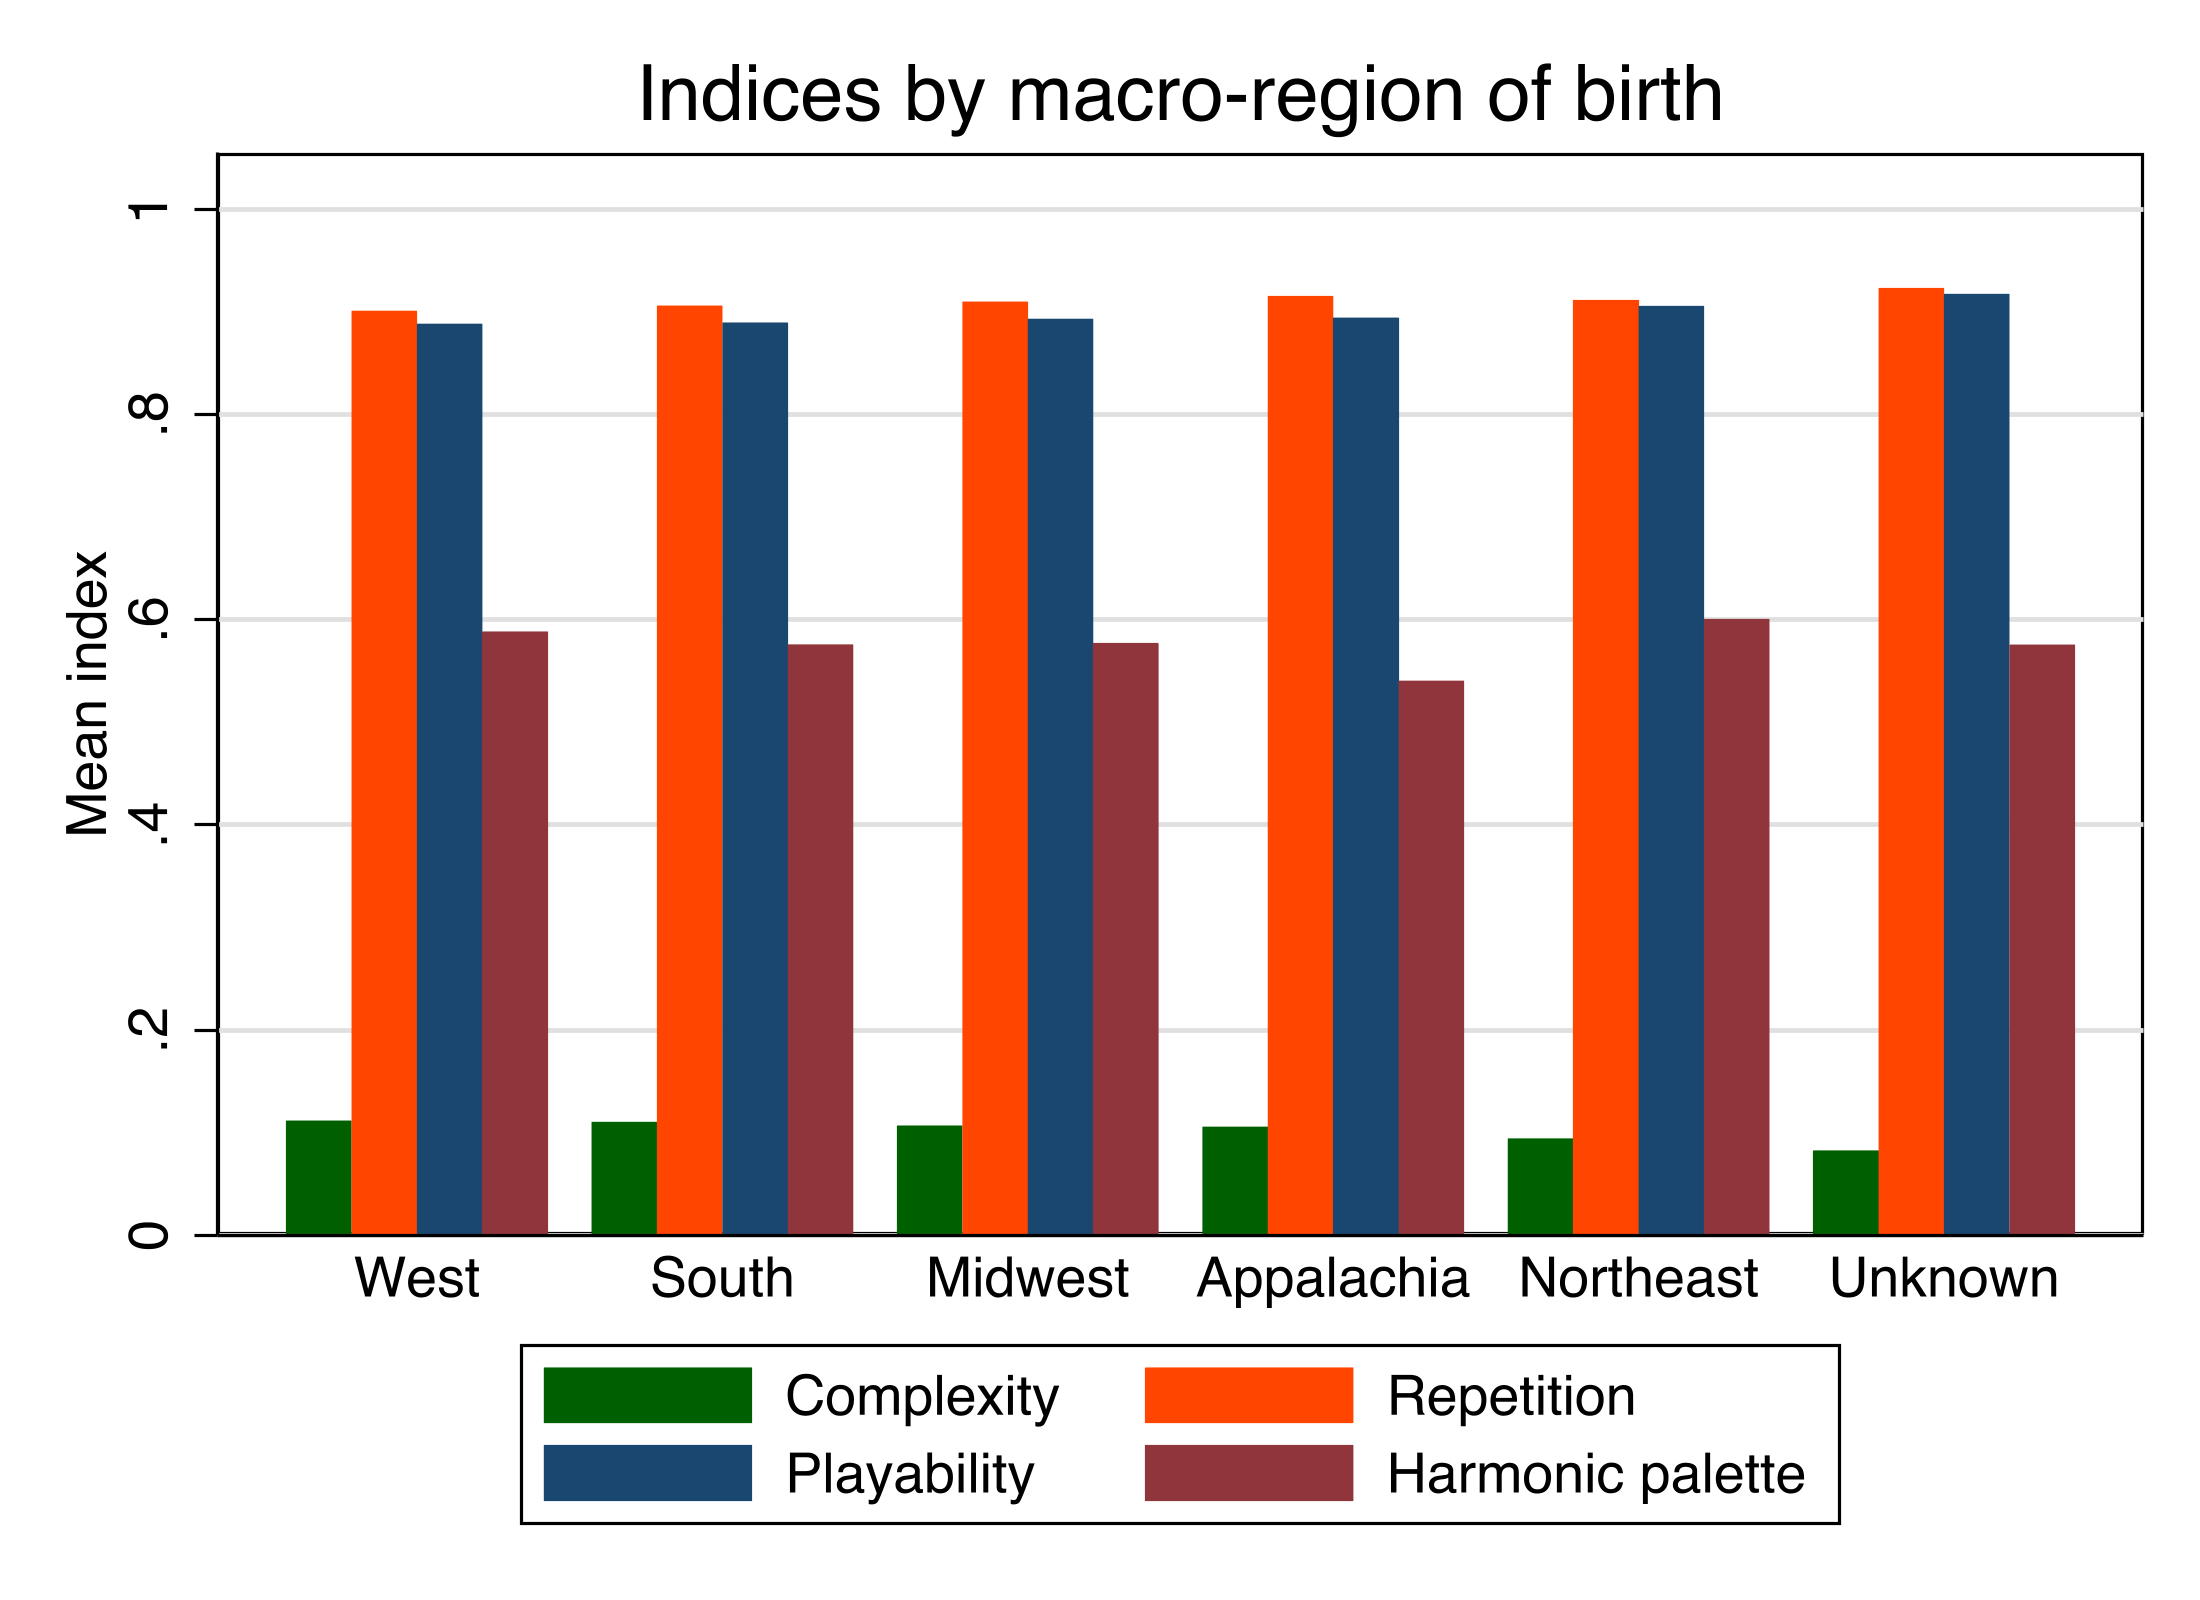
\includegraphics[width=0.92\textwidth]{analysis_outputs/graphs/10_indices_by_macro_region.png}
\caption{Figure 10. Index differences by macro-region}
\label{fig:geo_indices}
\end{figure}
Regional differences are large enough to survive omnibus tests for every reported measure. For instance, the omnibus p-values are $<0.001$ for complexity, $<0.001$ for repetition, and $<0.001$ for Billboard share. Appalachia stands out for repetition and Billboard presence, the Northeast has the highest harmonic palette, and the 'Unknown' group mechanically tops playability and structure variation, likely reflecting metadata selection rather than a clear cultural region.

\paragraph{Stata code used for the figure.}
\begin{lstlisting}
graph bar complexity repetition playability harmonic_palette, ///
    over(macro_region_clean, sort(1) descending) ///
    title("Indices by macro-region of birth") ///
    ytitle("Mean index") ///
    legend(order(1 "Complexity" 2 "Repetition" 3 "Playability" 4 "Harmonic palette") cols(2))
graph export "`graph_dir'/10_indices_by_macro_region.png", replace width(2200)
\end{lstlisting}



\subsection{Figure 11. Observation count by artist generation}
\begin{figure}[H]
\centering
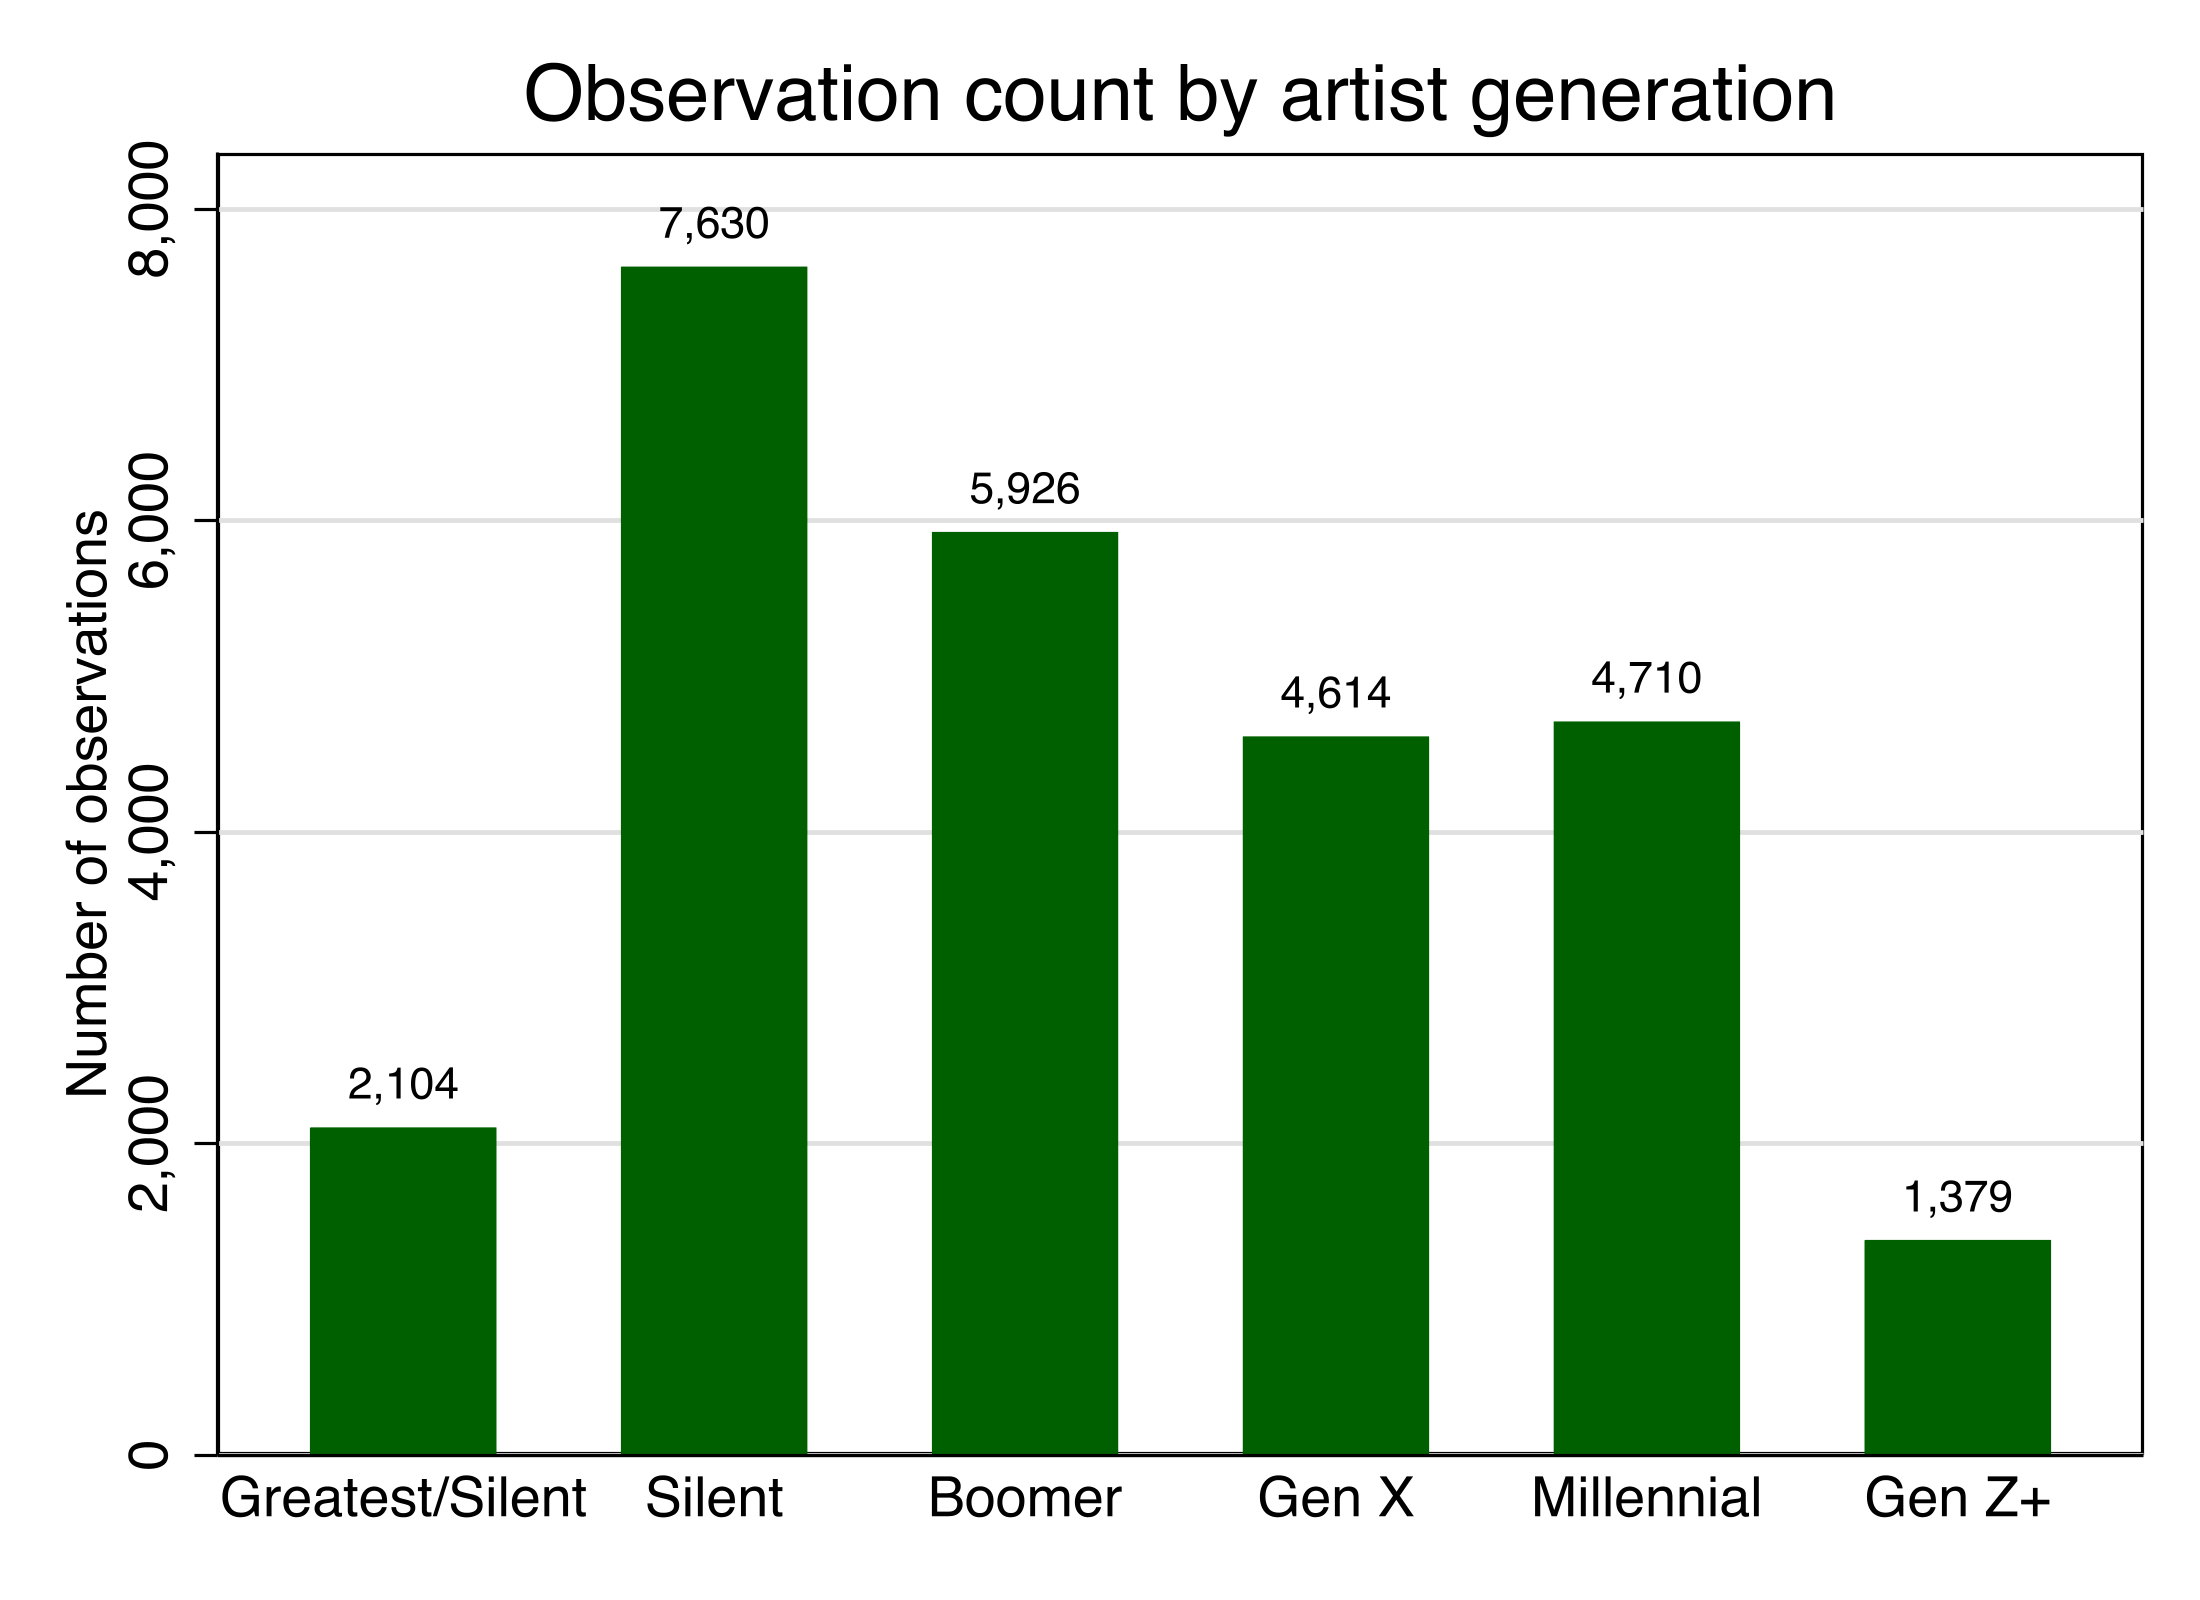
\includegraphics[width=0.92\textwidth]{analysis_outputs/graphs/11_generation_distribution.png}
\caption{Figure 11. Observation count by artist generation}
\label{fig:generation_counts}
\end{figure}
Generationally, the sample is anchored by older cohorts: the Silent generation contributes 7,630 songs and Boomers contribute 5,926. Millennials and Gen Z+ are smaller in raw count but become disproportionately important in the most recent period. As with the regional count figure, this panel is descriptive and should be paired with the inferential contrast in Figure~\ref{fig:generation_indices}.

\paragraph{Stata code used for the figure.}
\begin{lstlisting}
graph bar n_tabs, ///
    over(generation_group, relabel(1 "Greatest/Silent" 2 "Silent" 3 "Boomer" 4 "Gen X" 5 "Millennial" 6 "Gen Z+")) ///
    title("Observation count by artist generation") ///
    ytitle("Number of observations") blabel(bar, format(%9.0fc))
graph export "`graph_dir'/11_generation_distribution.png", replace width(2200)
\end{lstlisting}



\subsection{Figure 12. Index differences by artist generation}
\begin{figure}[H]
\centering
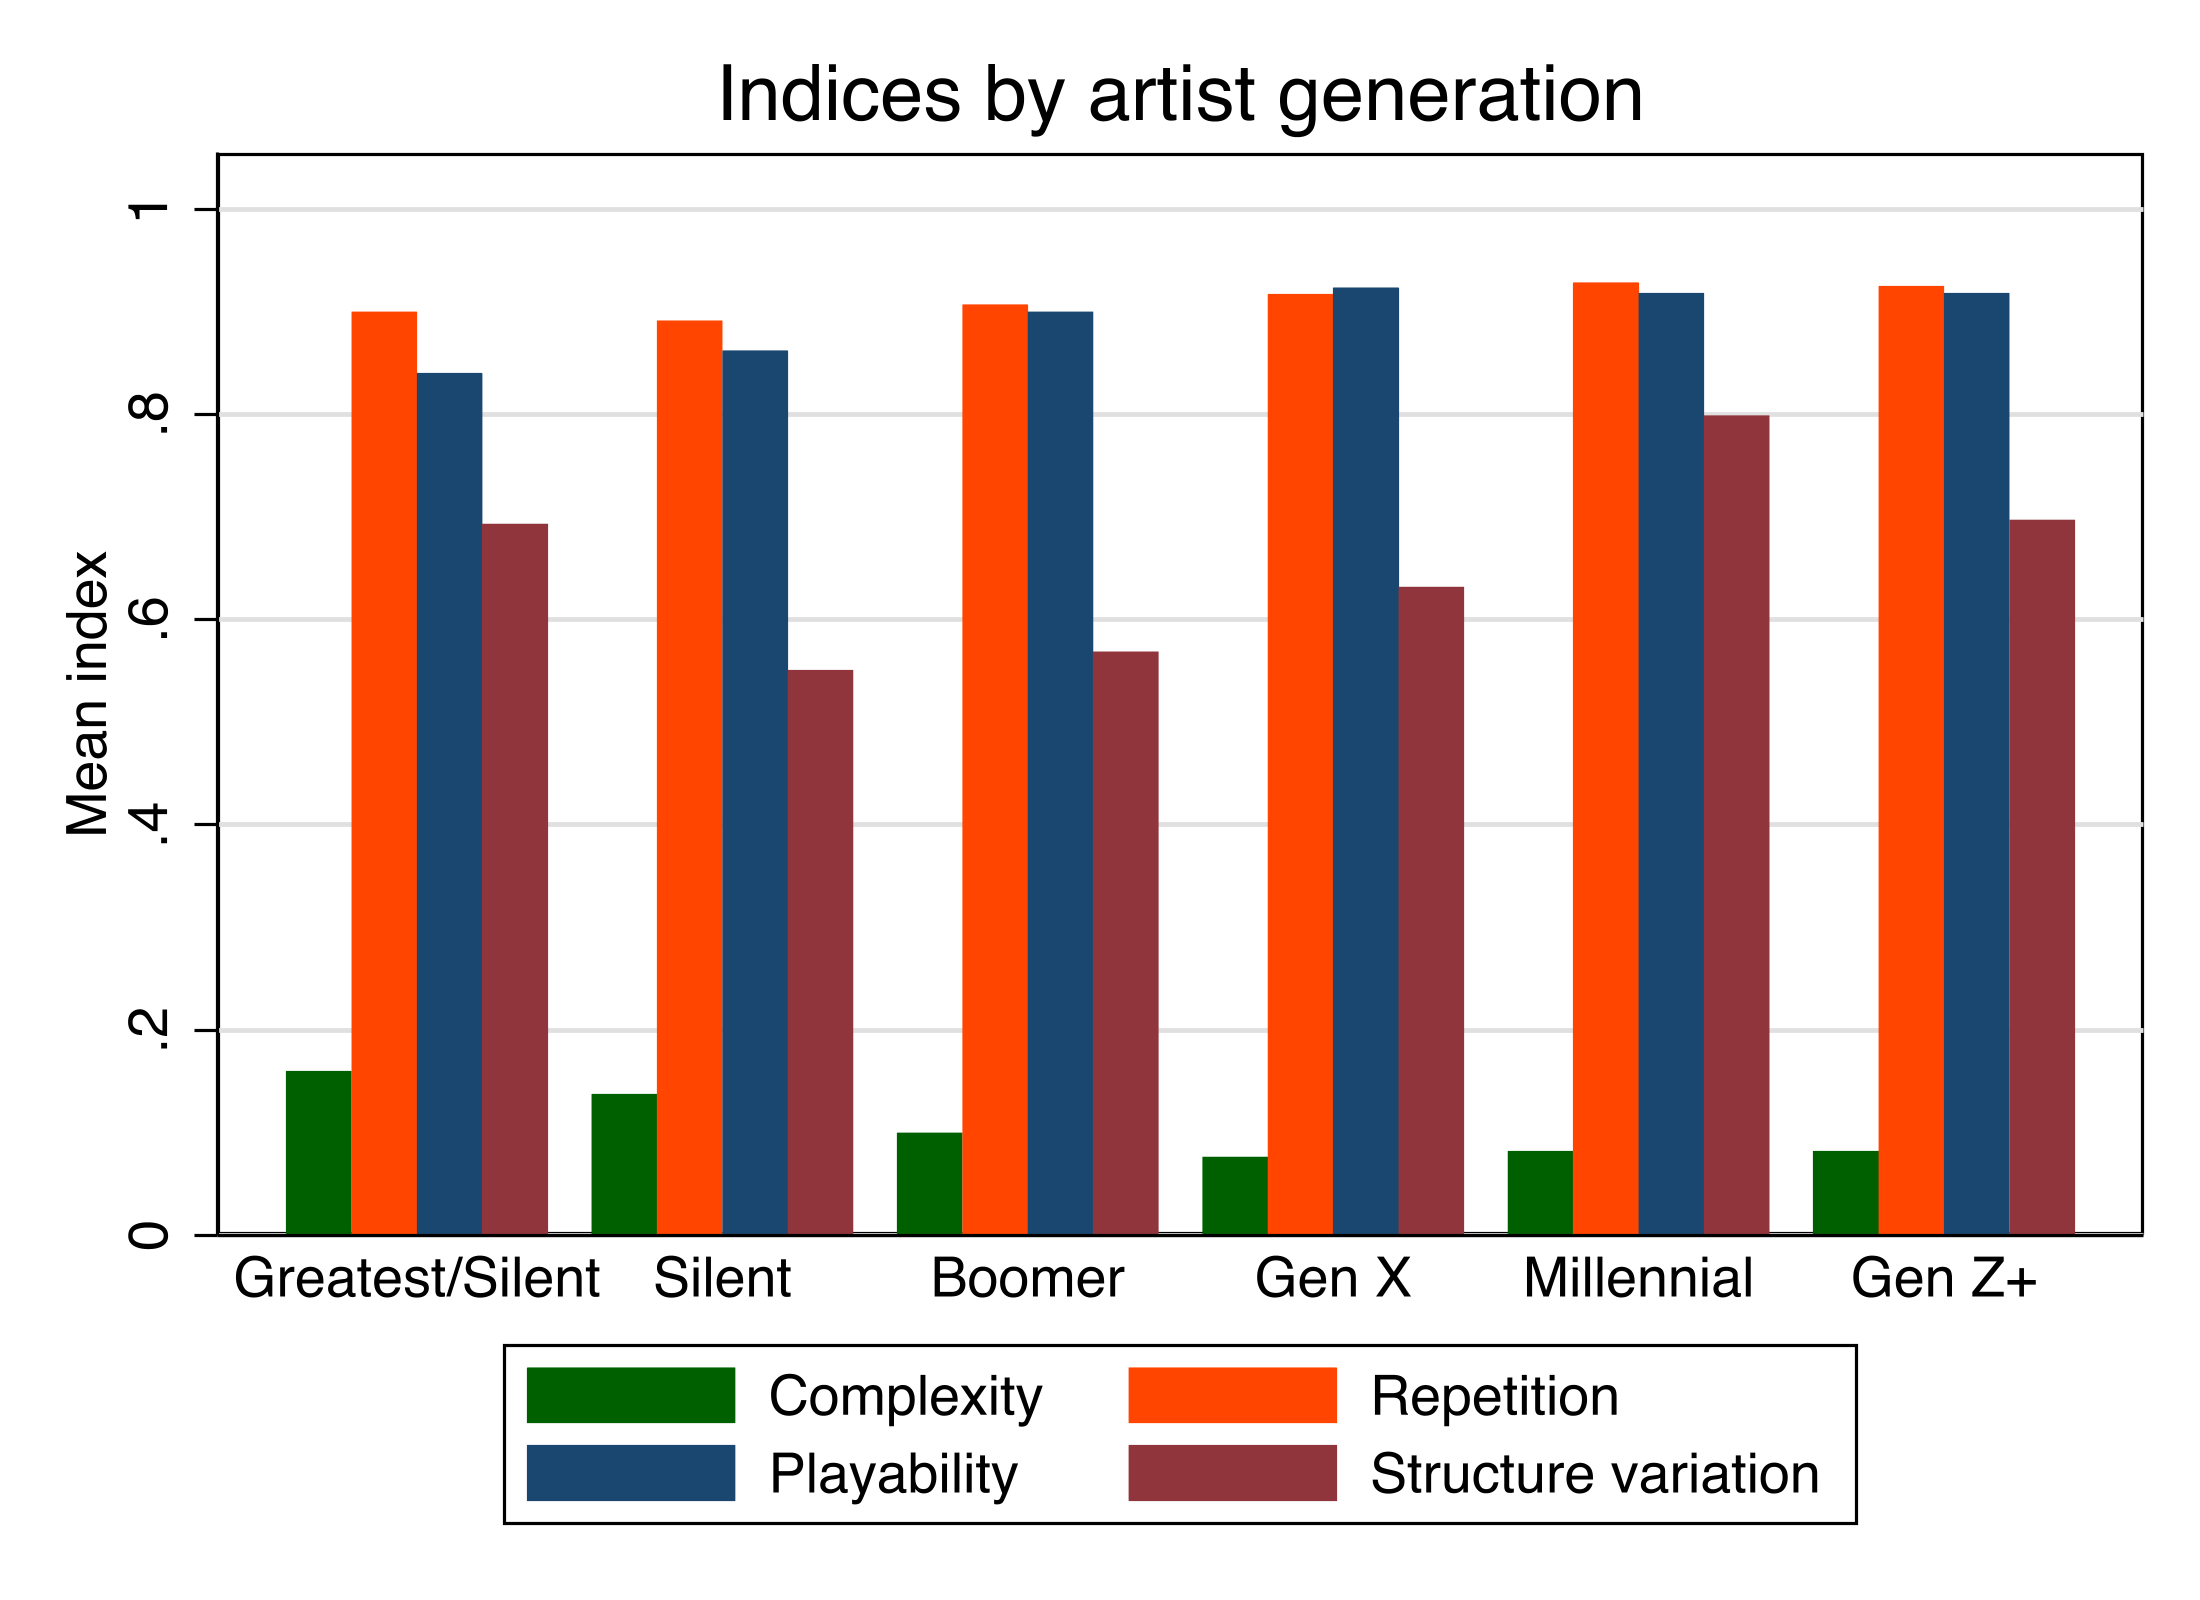
\includegraphics[width=0.92\textwidth]{analysis_outputs/graphs/12_indices_by_generation.png}
\caption{Figure 12. Index differences by artist generation}
\label{fig:generation_indices}
\end{figure}
Generational contrasts are extremely strong statistically. Complexity, repetition, playability, structure variation, Billboard share and upload-release gap all reject equality across generations with p-values effectively at zero. Substantively, older cohorts such as Greatest/Silent are much more complex and much less playable, while Millennials and Gen Z+ are more repetitive, easier to play, and structurally more varied. Millennials also show the highest structure variation, whereas Gen Z+ combines high repetition with very low average age at release.

\paragraph{Stata code used for the figure.}
\begin{lstlisting}
graph bar complexity repetition playability structure_variation, ///
    over(generation_group, relabel(1 "Greatest/Silent" 2 "Silent" 3 "Boomer" 4 "Gen X" 5 "Millennial" 6 "Gen Z+")) ///
    title("Indices by artist generation") ///
    ytitle("Mean index") ///
    legend(order(1 "Complexity" 2 "Repetition" 3 "Playability" 4 "Structure variation") cols(2))
graph export "`graph_dir'/12_indices_by_generation.png", replace width(2200)
\end{lstlisting}


\begin{table}[H]
\centering
\caption{Trend test for annual song counts}
\label{tab:count_trend}
\begin{tabular}{lcccc}
\toprule
Outcome & Slope per year & Slope per decade & p-value & N years \\
\midrule
Song count & 9.396 & 93.958 & $<0.001$ & 81 \\
\bottomrule
\end{tabular}
\end{table}

\begin{landscape}
\begin{table}[H]
\centering
\caption{Time-trend tests in the country-only sample}
\label{tab:time_trends}
\begin{tabular}{lcccc}
\toprule
Outcome & Slope per year & Slope per decade & p-value & N \\
\midrule
Complexity & -0.0012 & -0.0123 & $<0.001$ & 27,037 \\
Repetition & 0.0007 & 0.0068 & $<0.001$ & 27,037 \\
Melodicness & 0.0011 & 0.0107 & $<0.001$ & 27,037 \\
Energy & 0.0002 & 0.0018 & $<0.001$ & 27,037 \\
Finger movement & 0.0042 & 0.0420 & $<0.001$ & 27,037 \\
Disruption & 0.0007 & 0.0065 & $<0.001$ & 27,037 \\
Root stability & -0.0005 & -0.0046 & $<0.001$ & 27,037 \\
Intra-root variation & -0.0006 & -0.0064 & $<0.001$ & 27,037 \\
Harmonic palette & -0.0005 & -0.0045 & $<0.001$ & 27,037 \\
Loop strength & 0.0076 & 0.0758 & $<0.001$ & 27,037 \\
Structure variation & 0.0050 & 0.0500 & $<0.001$ & 27,037 \\
Playability & 0.0012 & 0.0123 & $<0.001$ & 27,037 \\
Harmonic softness & -0.0016 & -0.0160 & $<0.001$ & 27,037 \\
BPM & -0.0863 & -0.8630 & 0.060 & 3,803 \\
Billboard year-end share & 0.0008 & 0.0076 & $<0.001$ & 27,042 \\
Upload-release gap & -0.9636 & -9.6361 & $<0.001$ & 27,042 \\
\bottomrule
\end{tabular}
\end{table}
\end{landscape}

\begin{table}[H]
\centering
\caption{Trend tests for broad-sample genre shares}
\label{tab:genre_trends}
\begin{tabular}{lcc}
\toprule
Outcome & Slope per decade & p-value \\
\midrule
Country share & -0.0003 & 0.744 \\
Rock share & 0.0004 & 0.394 \\
Pop share & -0.0002 & 0.750 \\
Folk share & -0.0001 & 0.633 \\
Hip hop share & 0.0002 & 0.041 \\
R\&B/Funk/Soul share & -0.0000 & 0.626 \\
\bottomrule
\end{tabular}
\end{table}

\begin{table}[H]
\centering
\caption{Trend tests for first-chord shares}
\label{tab:chord_trends}
\begin{tabular}{lcc}
\toprule
Outcome & Slope per decade & p-value \\
\midrule
G share & -0.0002 & 0.282 \\
C share & -0.0002 & 0.848 \\
D share & 0.0004 & 0.146 \\
A share & -0.0007 & 0.054 \\
E share & -0.0004 & 0.019 \\
F share & 0.0001 & 0.710 \\
\bottomrule
\end{tabular}
\end{table}

\begin{table}[H]
\centering
\caption{Macro-region summary in the country-only sample}
\label{tab:geo}
\begin{tabular}{lcccccc}
\toprule
Macro-region & Songs & Artists & Complexity & Repetition & Playability & Billboard share \\
\midrule
South & 16,211 & 385 & 0.111 & 0.906 & 0.889 & 4.2\% \\
Appalachia & 4,344 & 148 & 0.106 & 0.915 & 0.894 & 6.3\% \\
Midwest & 2,320 & 101 & 0.107 & 0.910 & 0.893 & 3.4\% \\
Unknown & 1,865 & 115 & 0.083 & 0.923 & 0.917 & 5.0\% \\
West & 1,653 & 68 & 0.112 & 0.901 & 0.888 & 2.7\% \\
Northeast & 649 & 32 & 0.094 & 0.911 & 0.906 & 1.7\% \\
\bottomrule
\end{tabular}
\end{table}

\begin{table}[H]
\centering
\caption{Omnibus tests for macro-region differences}
\label{tab:geo_tests}
\begin{tabular}{lcc}
\toprule
Outcome & p-value & N \\
\midrule
Complexity & $<0.001$ & 27,037 \\
Repetition & $<0.001$ & 27,037 \\
Playability & $<0.001$ & 27,037 \\
Harmonic palette & $<0.001$ & 27,037 \\
Structure variation & $<0.001$ & 27,037 \\
Billboard year-end share & $<0.001$ & 27,042 \\
\bottomrule
\end{tabular}
\end{table}

\begin{landscape}
\begin{table}[H]
\centering
\caption{Generation summary in the country-only sample}
\label{tab:generation}
\begin{tabular}{lccccccc}
\toprule
Generation & Songs & Artists & Complexity & Repetition & Playability & Structure variation & Billboard share \\
\midrule
Greatest/Silent & 2,104 & 62 & 0.160 & 0.900 & 0.840 & 0.693 & 5.3\% \\
Silent & 7,630 & 154 & 0.138 & 0.891 & 0.862 & 0.551 & 1.3\% \\
Boomer & 5,926 & 161 & 0.100 & 0.907 & 0.900 & 0.569 & 3.0\% \\
Gen X & 4,614 & 164 & 0.077 & 0.917 & 0.923 & 0.632 & 6.5\% \\
Millennial & 4,710 & 201 & 0.082 & 0.928 & 0.918 & 0.799 & 7.6\% \\
Gen Z+ & 1,379 & 73 & 0.082 & 0.925 & 0.918 & 0.697 & 7.3\% \\
\bottomrule
\end{tabular}
\end{table}
\end{landscape}

\begin{table}[H]
\centering
\caption{Omnibus tests for generation differences}
\label{tab:generation_tests}
\begin{tabular}{lcc}
\toprule
Outcome & p-value & N \\
\midrule
Complexity & $<0.001$ & 26,358 \\
Repetition & $<0.001$ & 26,358 \\
Playability & $<0.001$ & 26,358 \\
Harmonic palette & $<0.001$ & 26,358 \\
Structure variation & $<0.001$ & 26,358 \\
Billboard year-end share & $<0.001$ & 26,363 \\
Upload-release gap & $<0.001$ & 26,363 \\
\bottomrule
\end{tabular}
\end{table}


\section{Interpretive summary}
Several regularities emerge repeatedly across the figures and tests.

\begin{enumerate}
\item Modern country songs in this tab-based sample become easier to play and more repetitive, not more harmonically expansive.
\item The strongest secular movements are the rise in repetition, loop strength and structure variation, and the fall in complexity and harmonic softness.
\item Geographic heterogeneity is not cosmetic: macro-regional differences are significant for all core indices shown in the report.
\item Generational turnover matters at least as much as geography. Older generations encode a more complex and less playable harmonic language, while younger generations are associated with high repetition and contemporary platform timing.
\item The broad artist-based sample is not enough for substantive country-song inference; the country-only genre filter is necessary because the broad sample retains substantial rock and pop content in every decade.
\end{enumerate}

\section{Appendix A: Individual index figures}
The following gallery reports the one-variable annual figures generated by the loop below. The code is shared because each figure differs only by the index substituted into the loop.

\begin{lstlisting}
foreach idx in complexity repetition melodicness energy finger_movement disruption ///
               root_stability intra_root_variation harmonic_palette loop_strength ///
               structure_variation playability harmonic_softness {
    twoway ///
        (line `idx' release_year, lcolor(navy) lwidth(medthick)), ///
        title("`idx' by release year") ///
        subtitle("Main analysis: country songs only") ///
        xtitle("Release year") ytitle("Mean index") ///
        xlabel(`analysis_start_year'(5)`analysis_end_year', angle(45)) ///
        xscale(range(`analysis_start_year' `analysis_end_year'))
    graph export "`graph_dir'/index_`idx'_by_release_year.png", replace width(2200)
}
\end{lstlisting}


\subsection{Complexity: individual annual trend}
\begin{figure}[H]
\centering
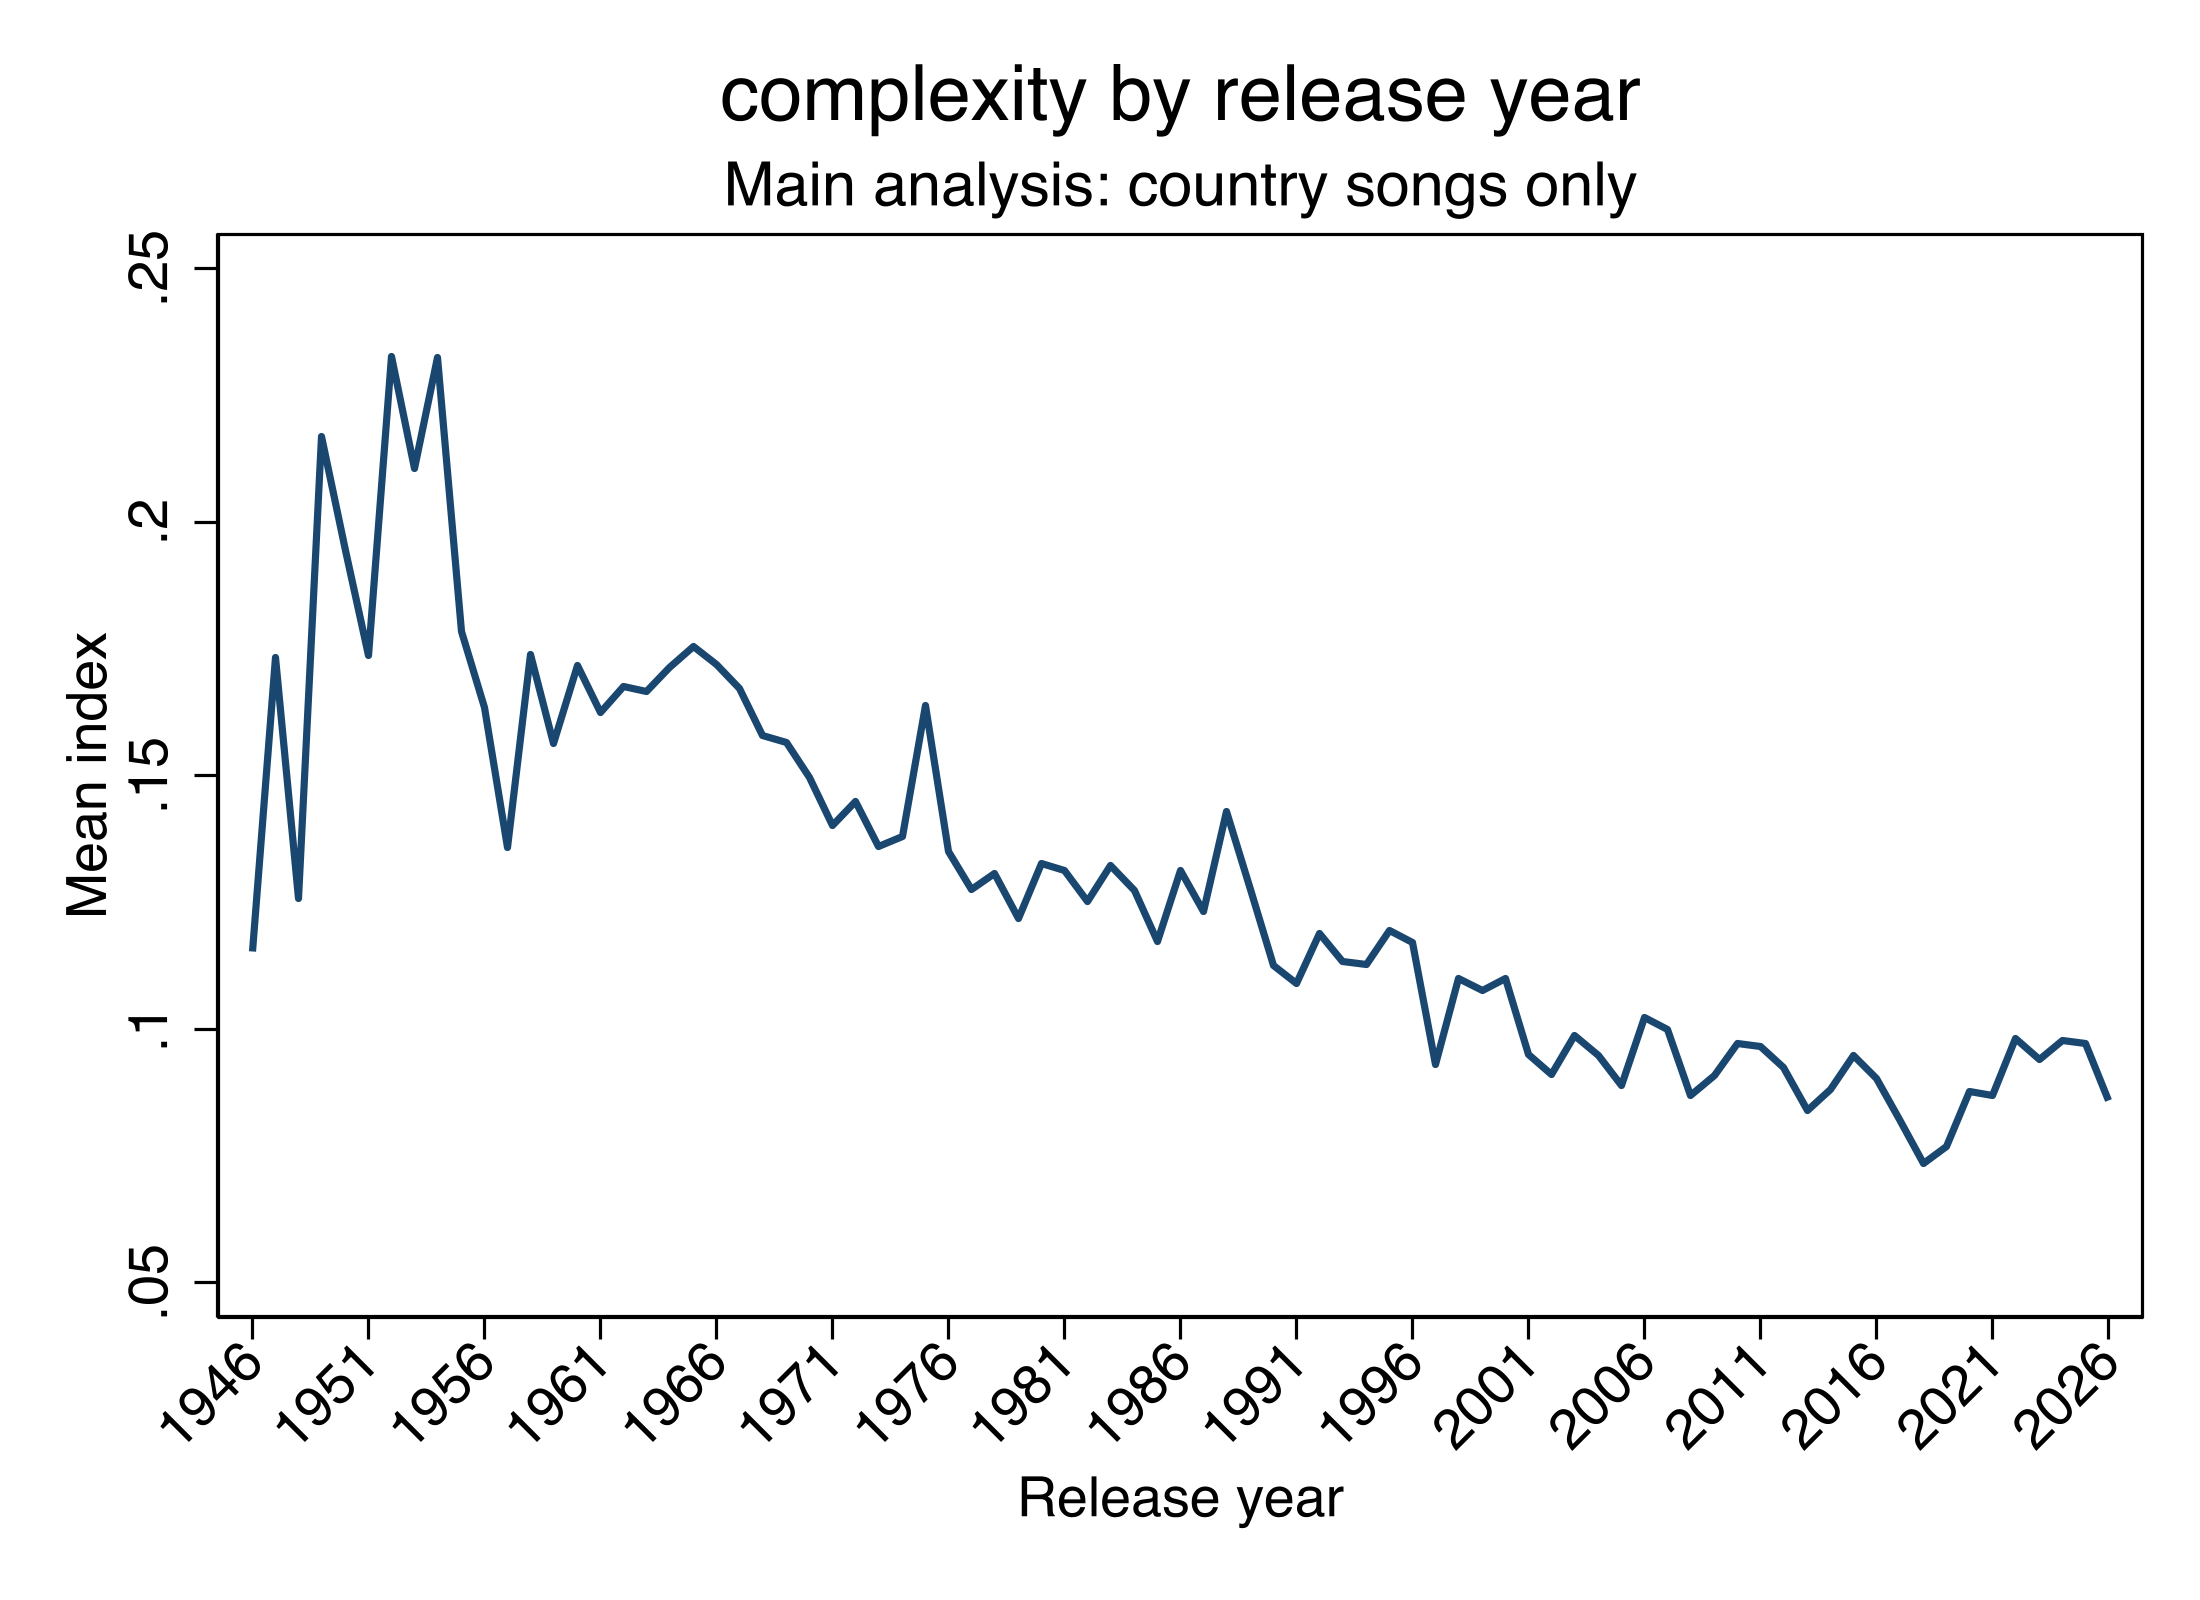
\includegraphics[width=0.88\textwidth]{analysis_outputs/graphs/index_complexity_by_release_year.png}
\caption{Individual annual trend for complexity}
\end{figure}
Complexity decreases by 0.0123 points per decade ($<0.001$).

\subsection{Repetition: individual annual trend}
\begin{figure}[H]
\centering
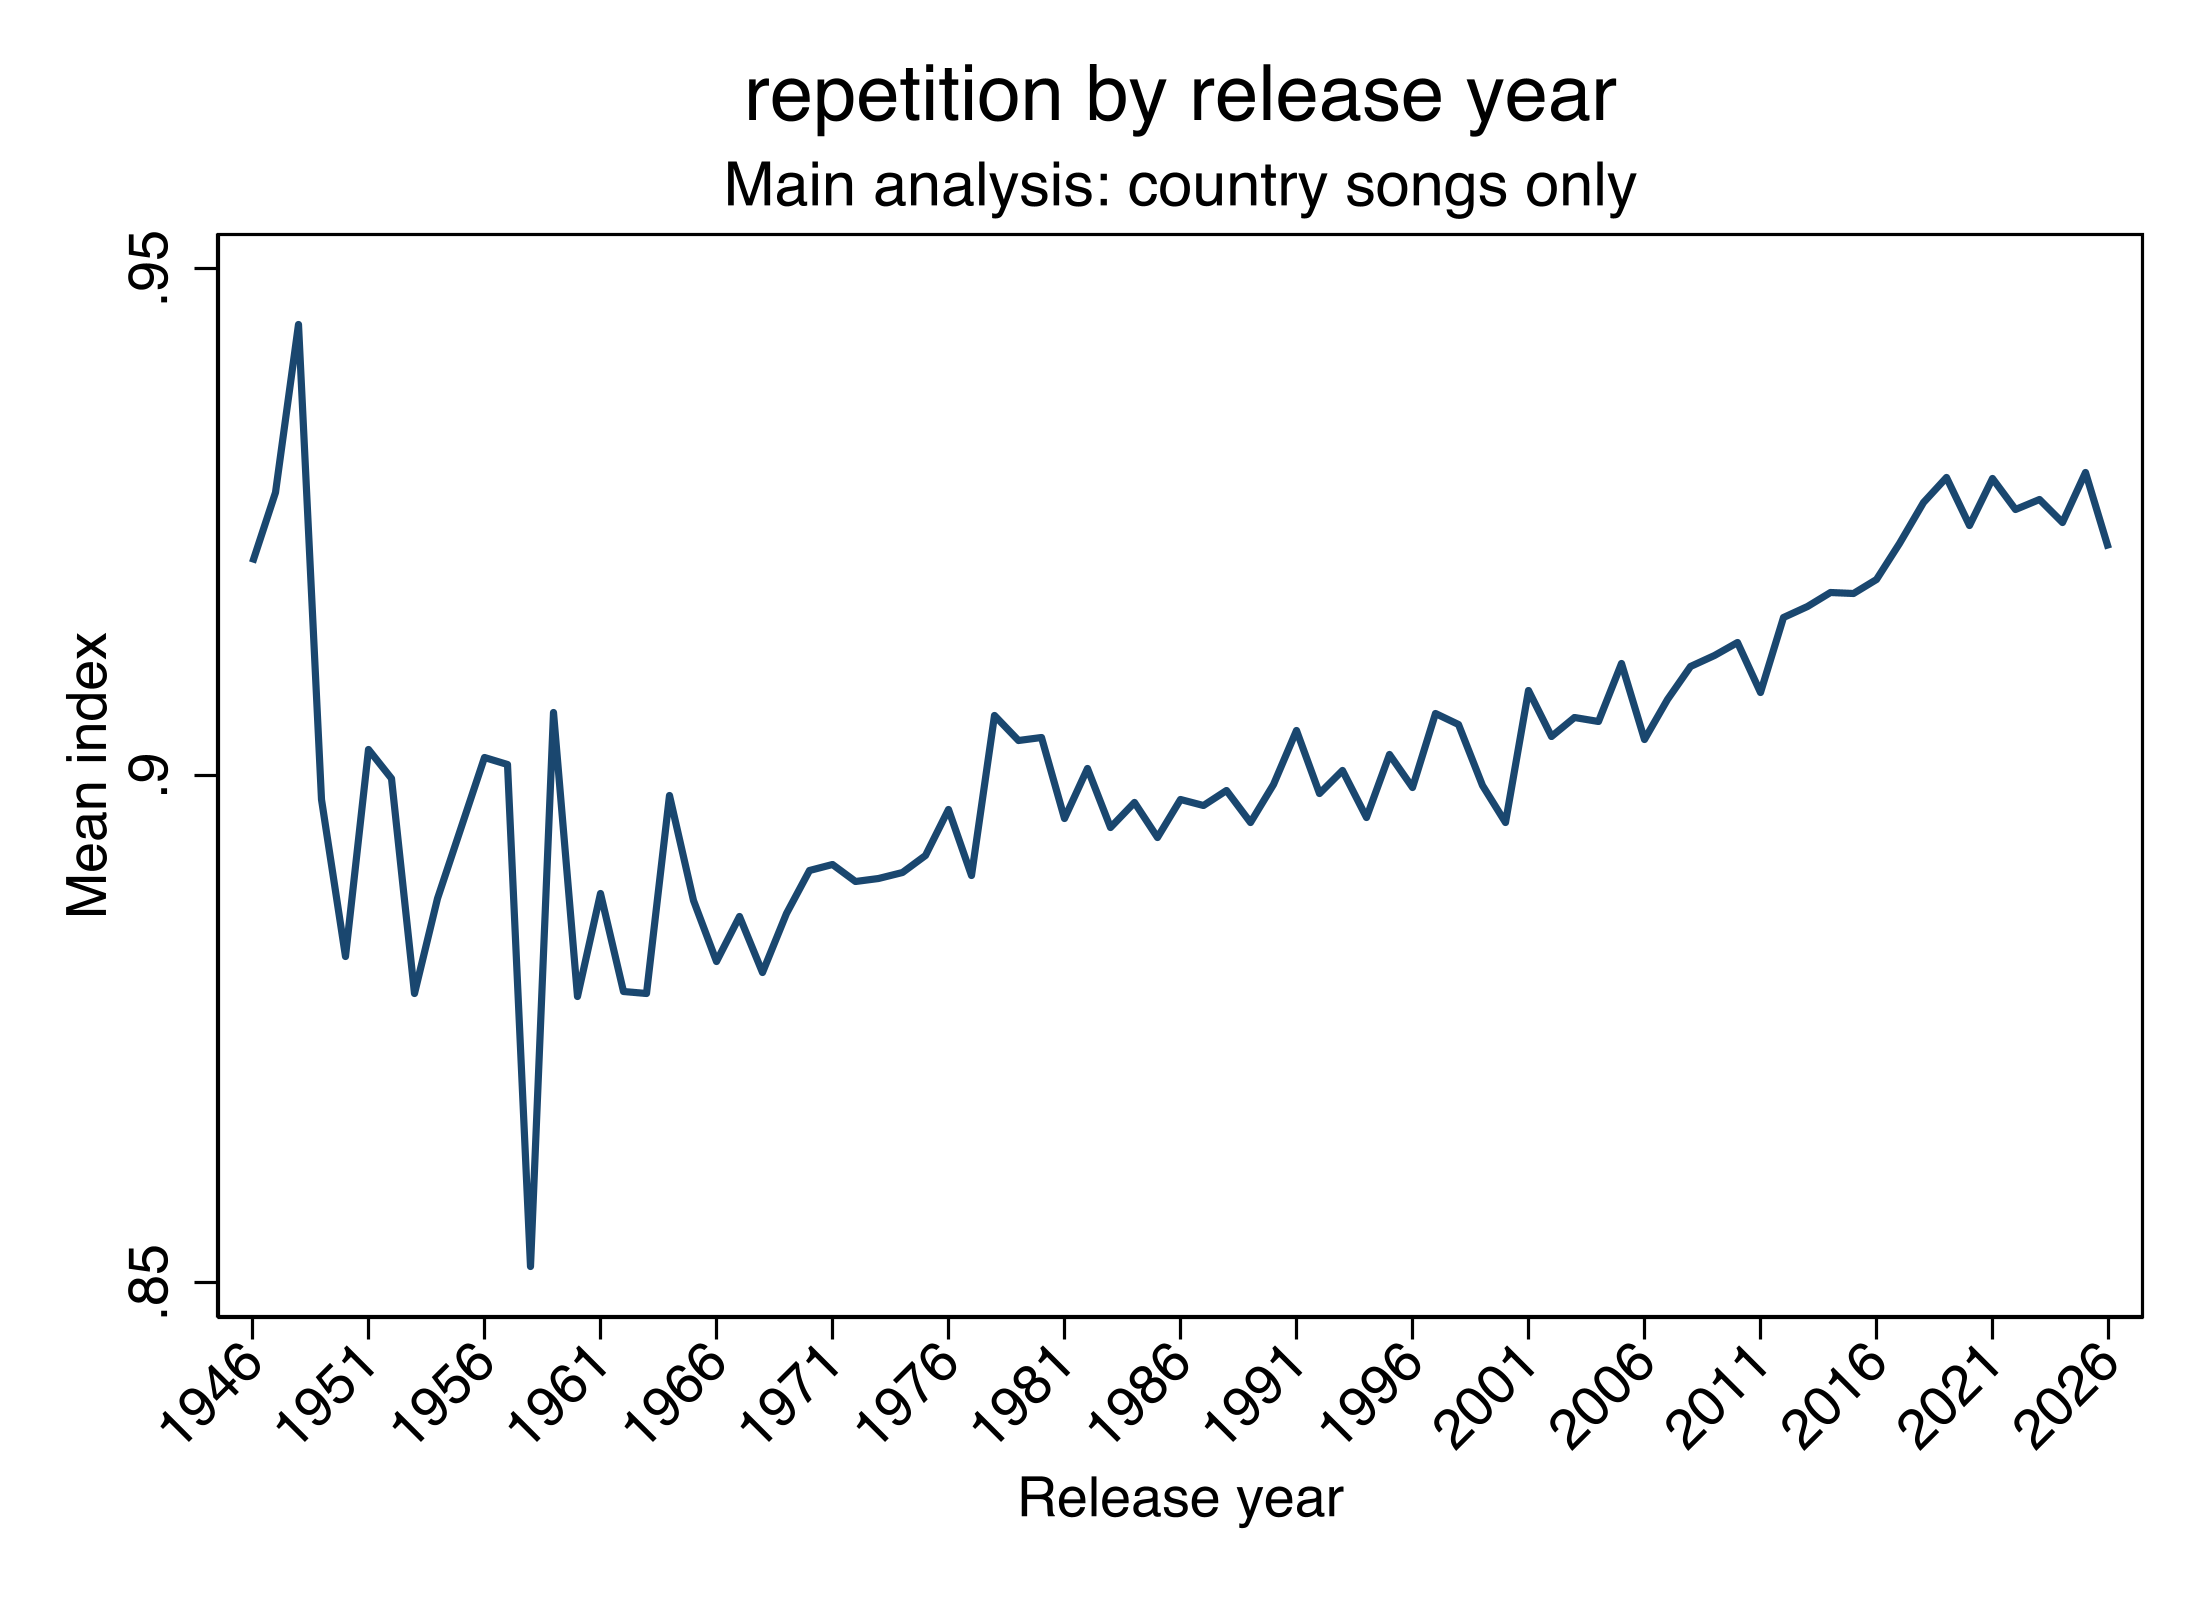
\includegraphics[width=0.88\textwidth]{analysis_outputs/graphs/index_repetition_by_release_year.png}
\caption{Individual annual trend for repetition}
\end{figure}
Repetition increases by 0.0068 points per decade ($<0.001$).

\subsection{Melodicness: individual annual trend}
\begin{figure}[H]
\centering
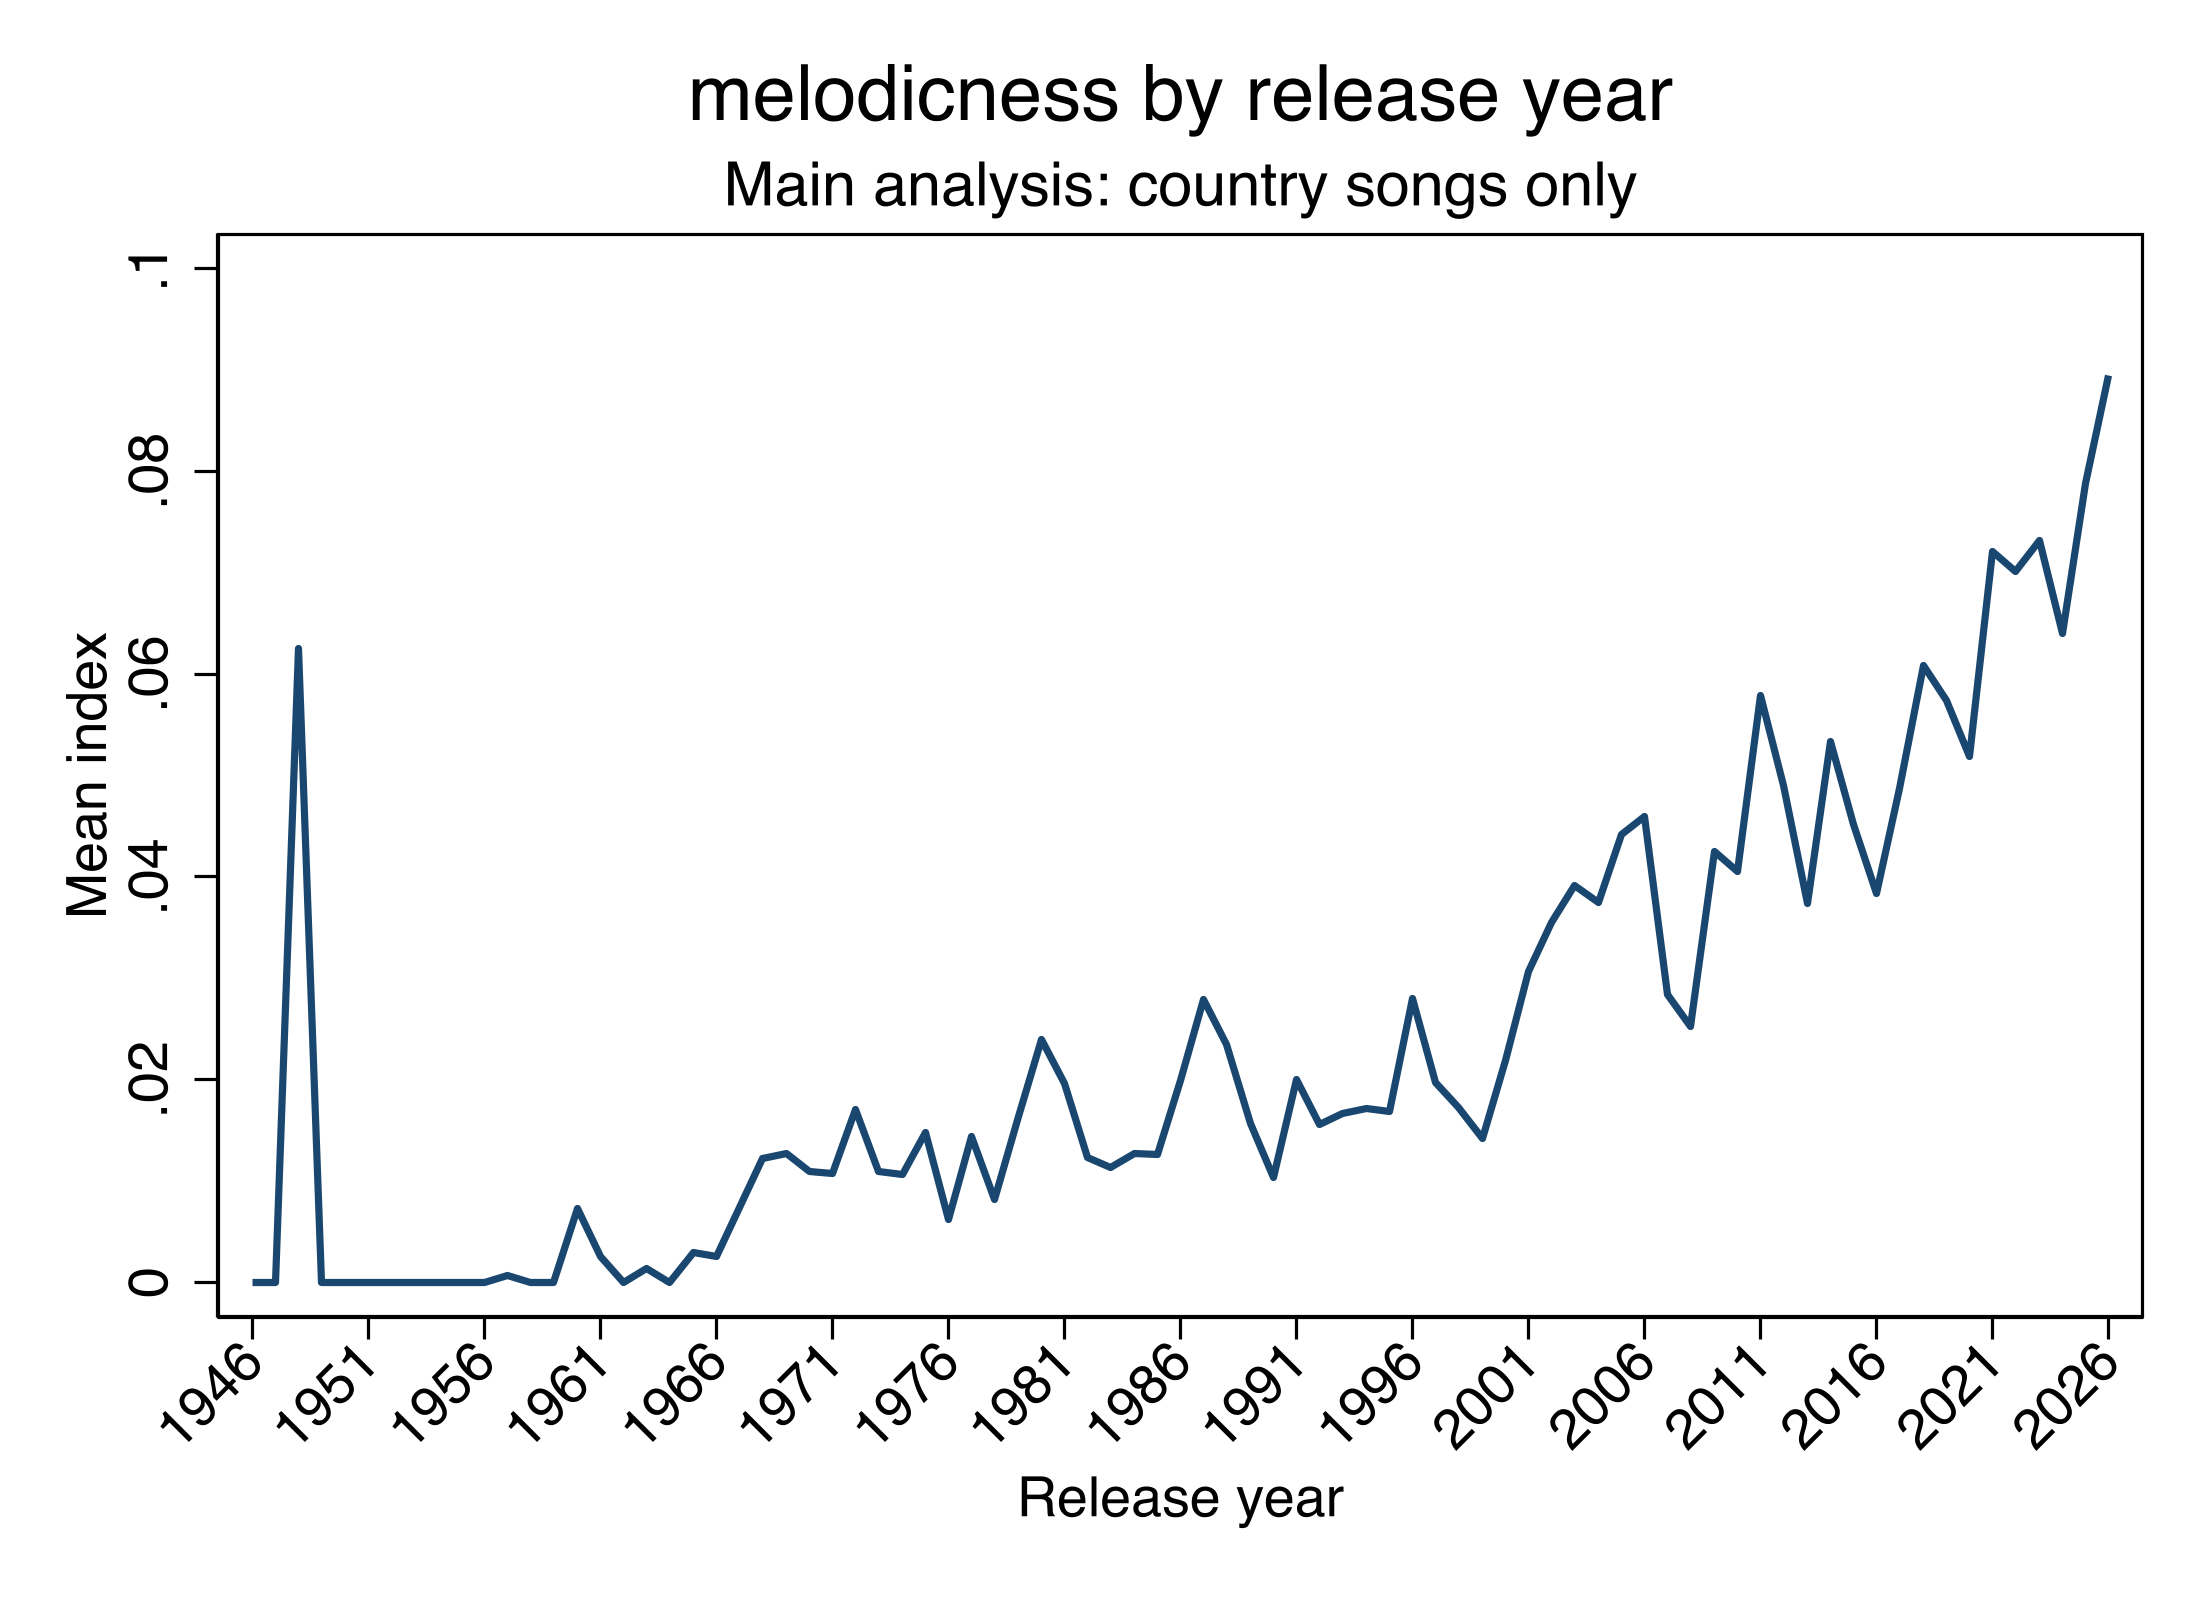
\includegraphics[width=0.88\textwidth]{analysis_outputs/graphs/index_melodicness_by_release_year.png}
\caption{Individual annual trend for melodicness}
\end{figure}
Melodicness increases by 0.0107 points per decade ($<0.001$).

\subsection{Energy: individual annual trend}
\begin{figure}[H]
\centering
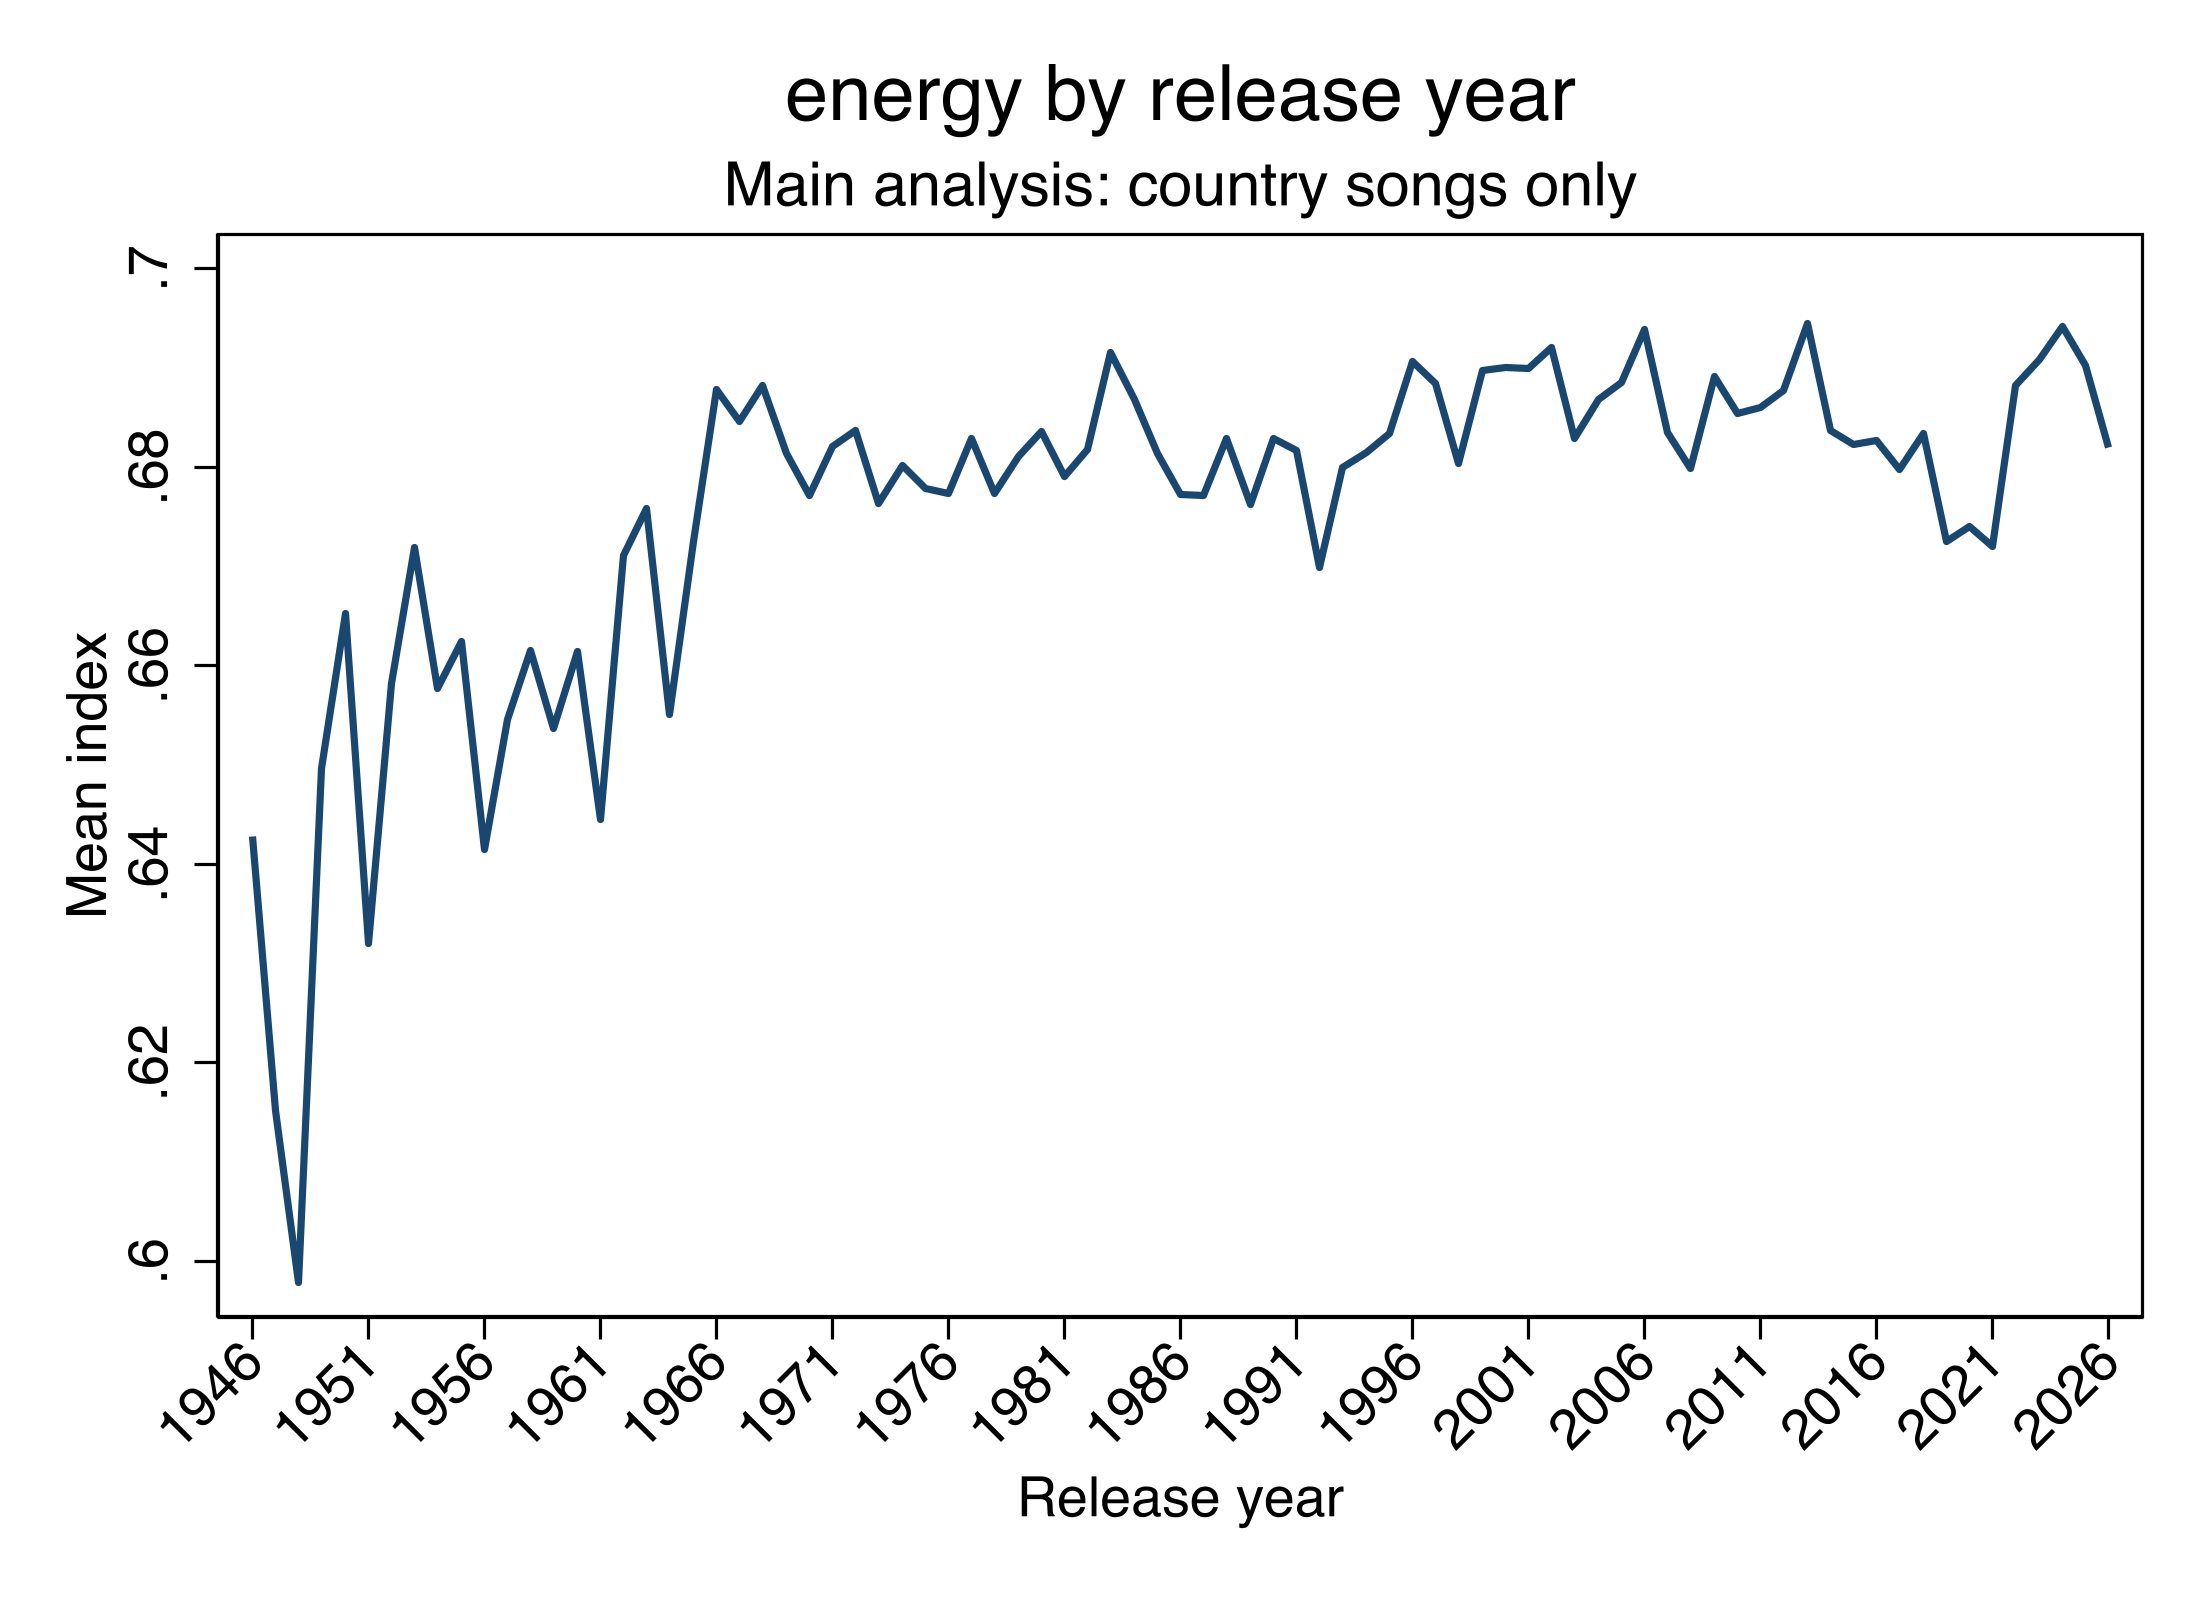
\includegraphics[width=0.88\textwidth]{analysis_outputs/graphs/index_energy_by_release_year.png}
\caption{Individual annual trend for energy}
\end{figure}
Energy increases by 0.0018 points per decade ($<0.001$).

\subsection{Finger movement: individual annual trend}
\begin{figure}[H]
\centering
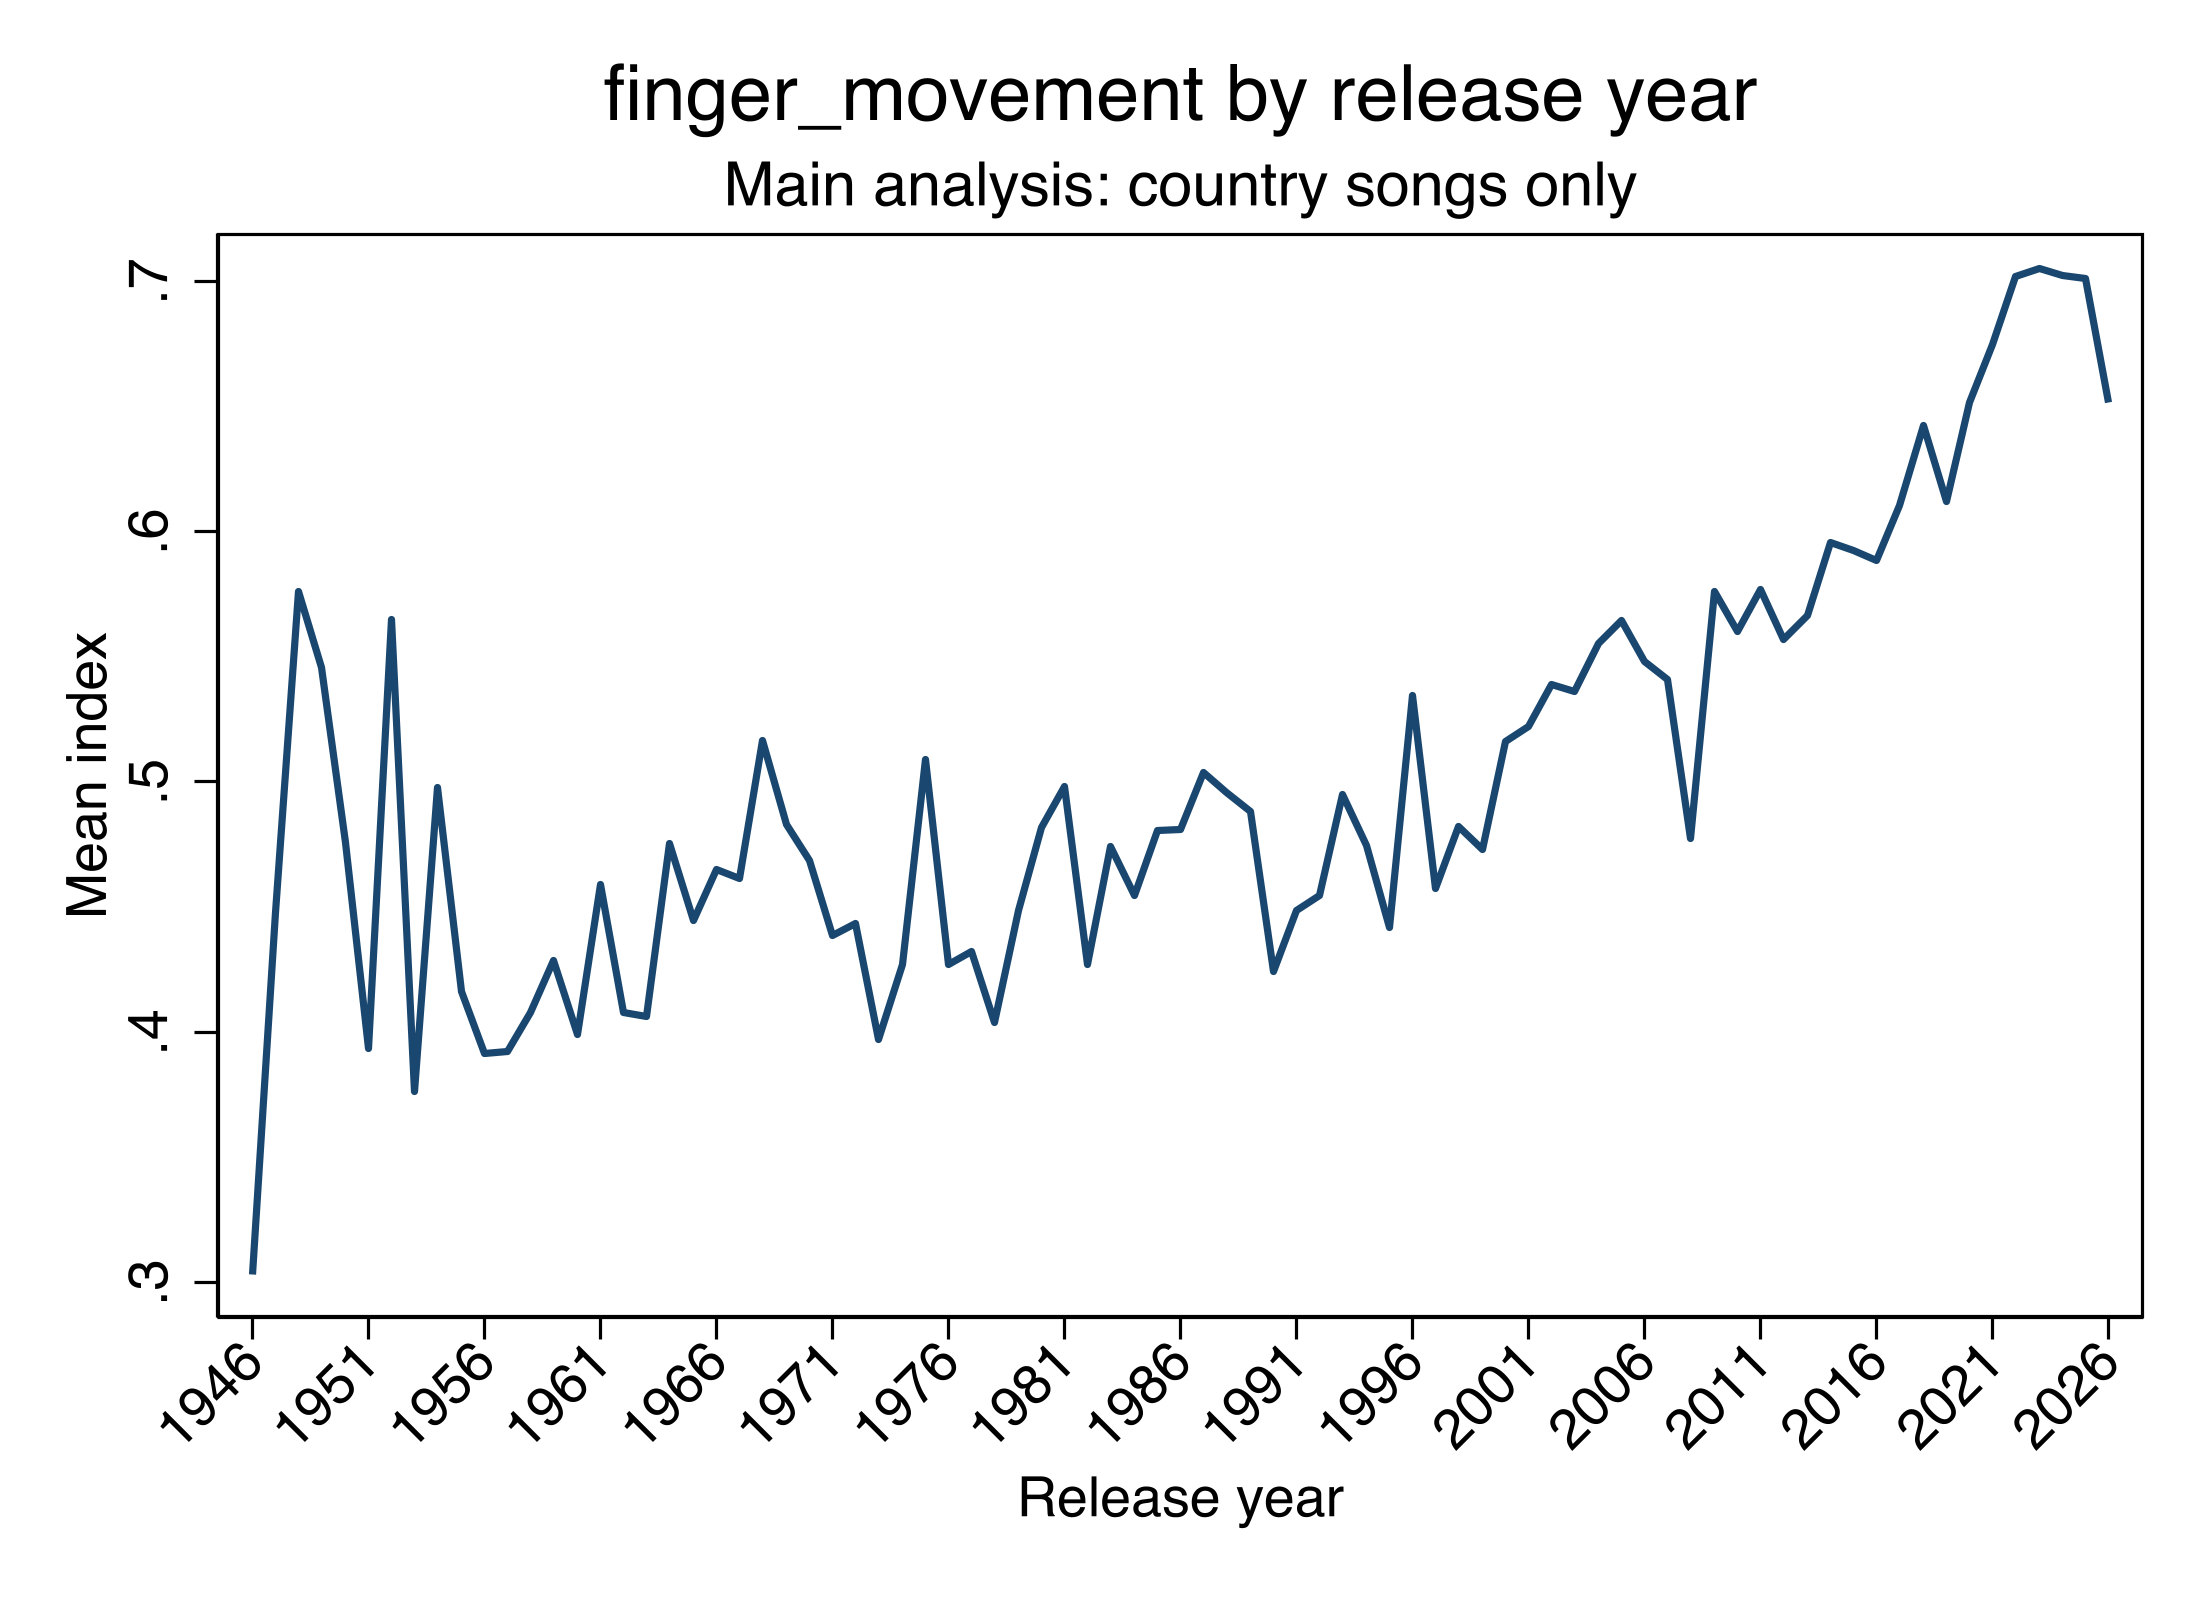
\includegraphics[width=0.88\textwidth]{analysis_outputs/graphs/index_finger_movement_by_release_year.png}
\caption{Individual annual trend for finger movement}
\end{figure}
Finger movement increases by 0.0420 points per decade ($<0.001$).

\subsection{Disruption: individual annual trend}
\begin{figure}[H]
\centering
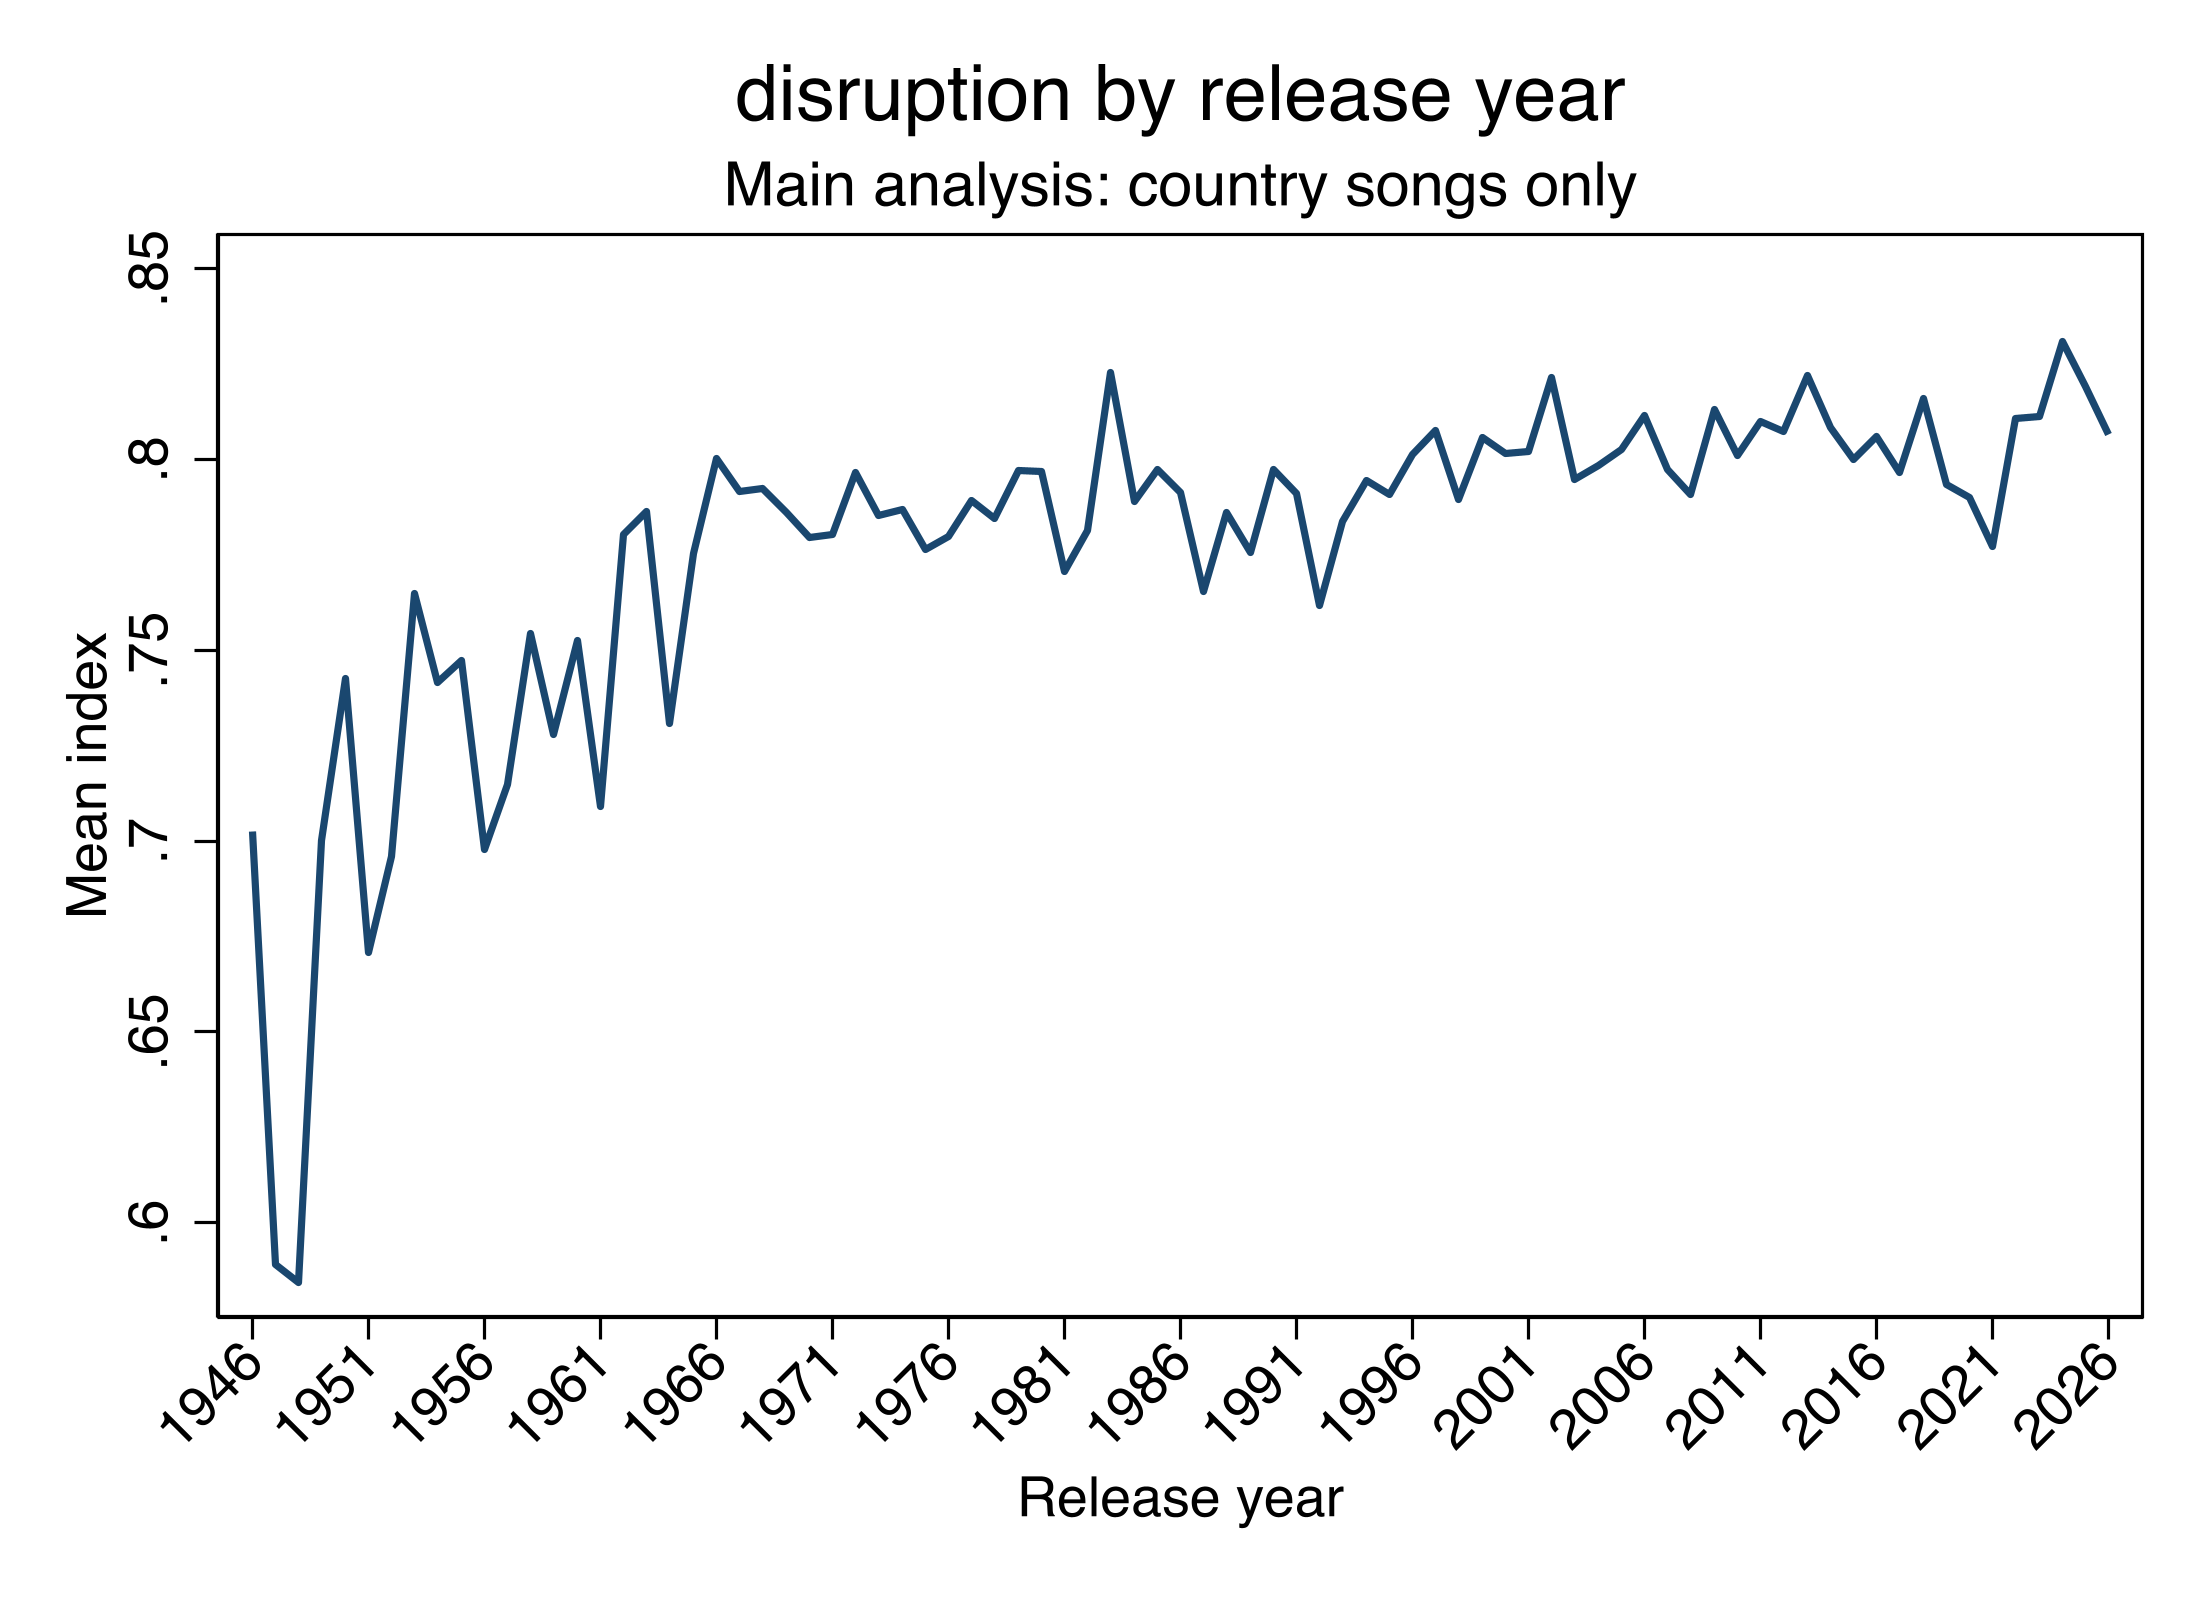
\includegraphics[width=0.88\textwidth]{analysis_outputs/graphs/index_disruption_by_release_year.png}
\caption{Individual annual trend for disruption}
\end{figure}
Disruption increases by 0.0065 points per decade ($<0.001$).

\subsection{Root stability: individual annual trend}
\begin{figure}[H]
\centering
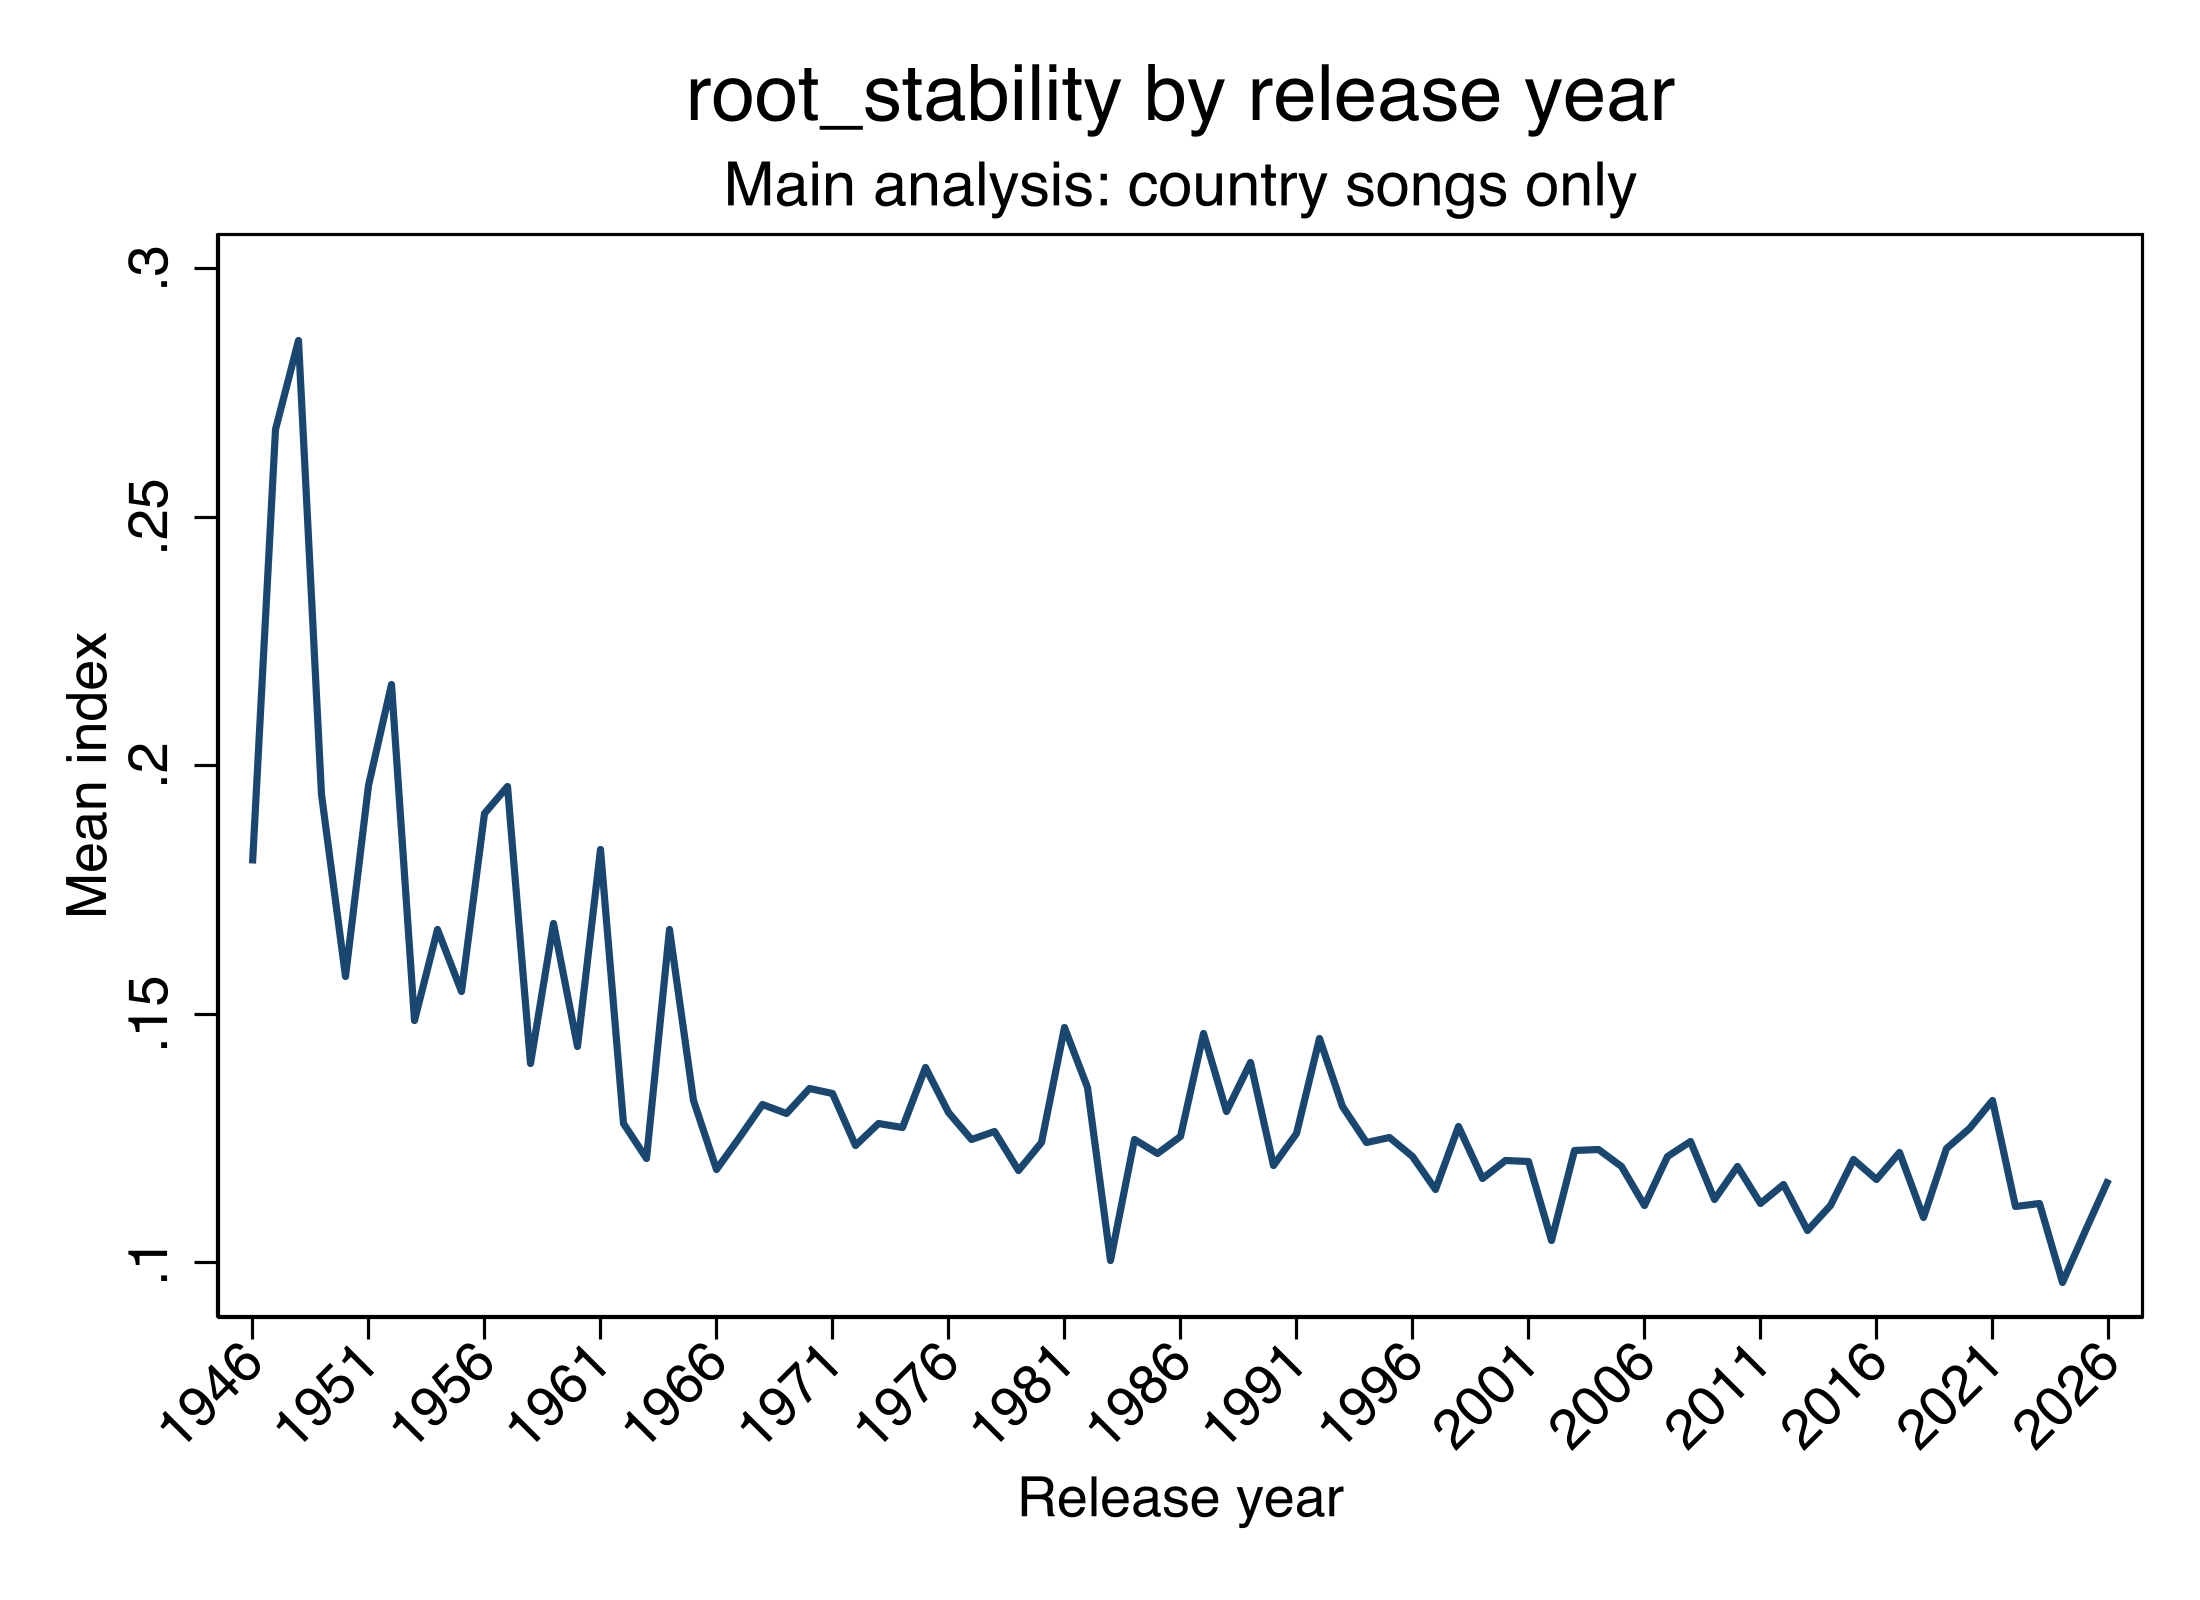
\includegraphics[width=0.88\textwidth]{analysis_outputs/graphs/index_root_stability_by_release_year.png}
\caption{Individual annual trend for root stability}
\end{figure}
Root stability decreases by 0.0046 points per decade ($<0.001$).

\subsection{Intra-root variation: individual annual trend}
\begin{figure}[H]
\centering
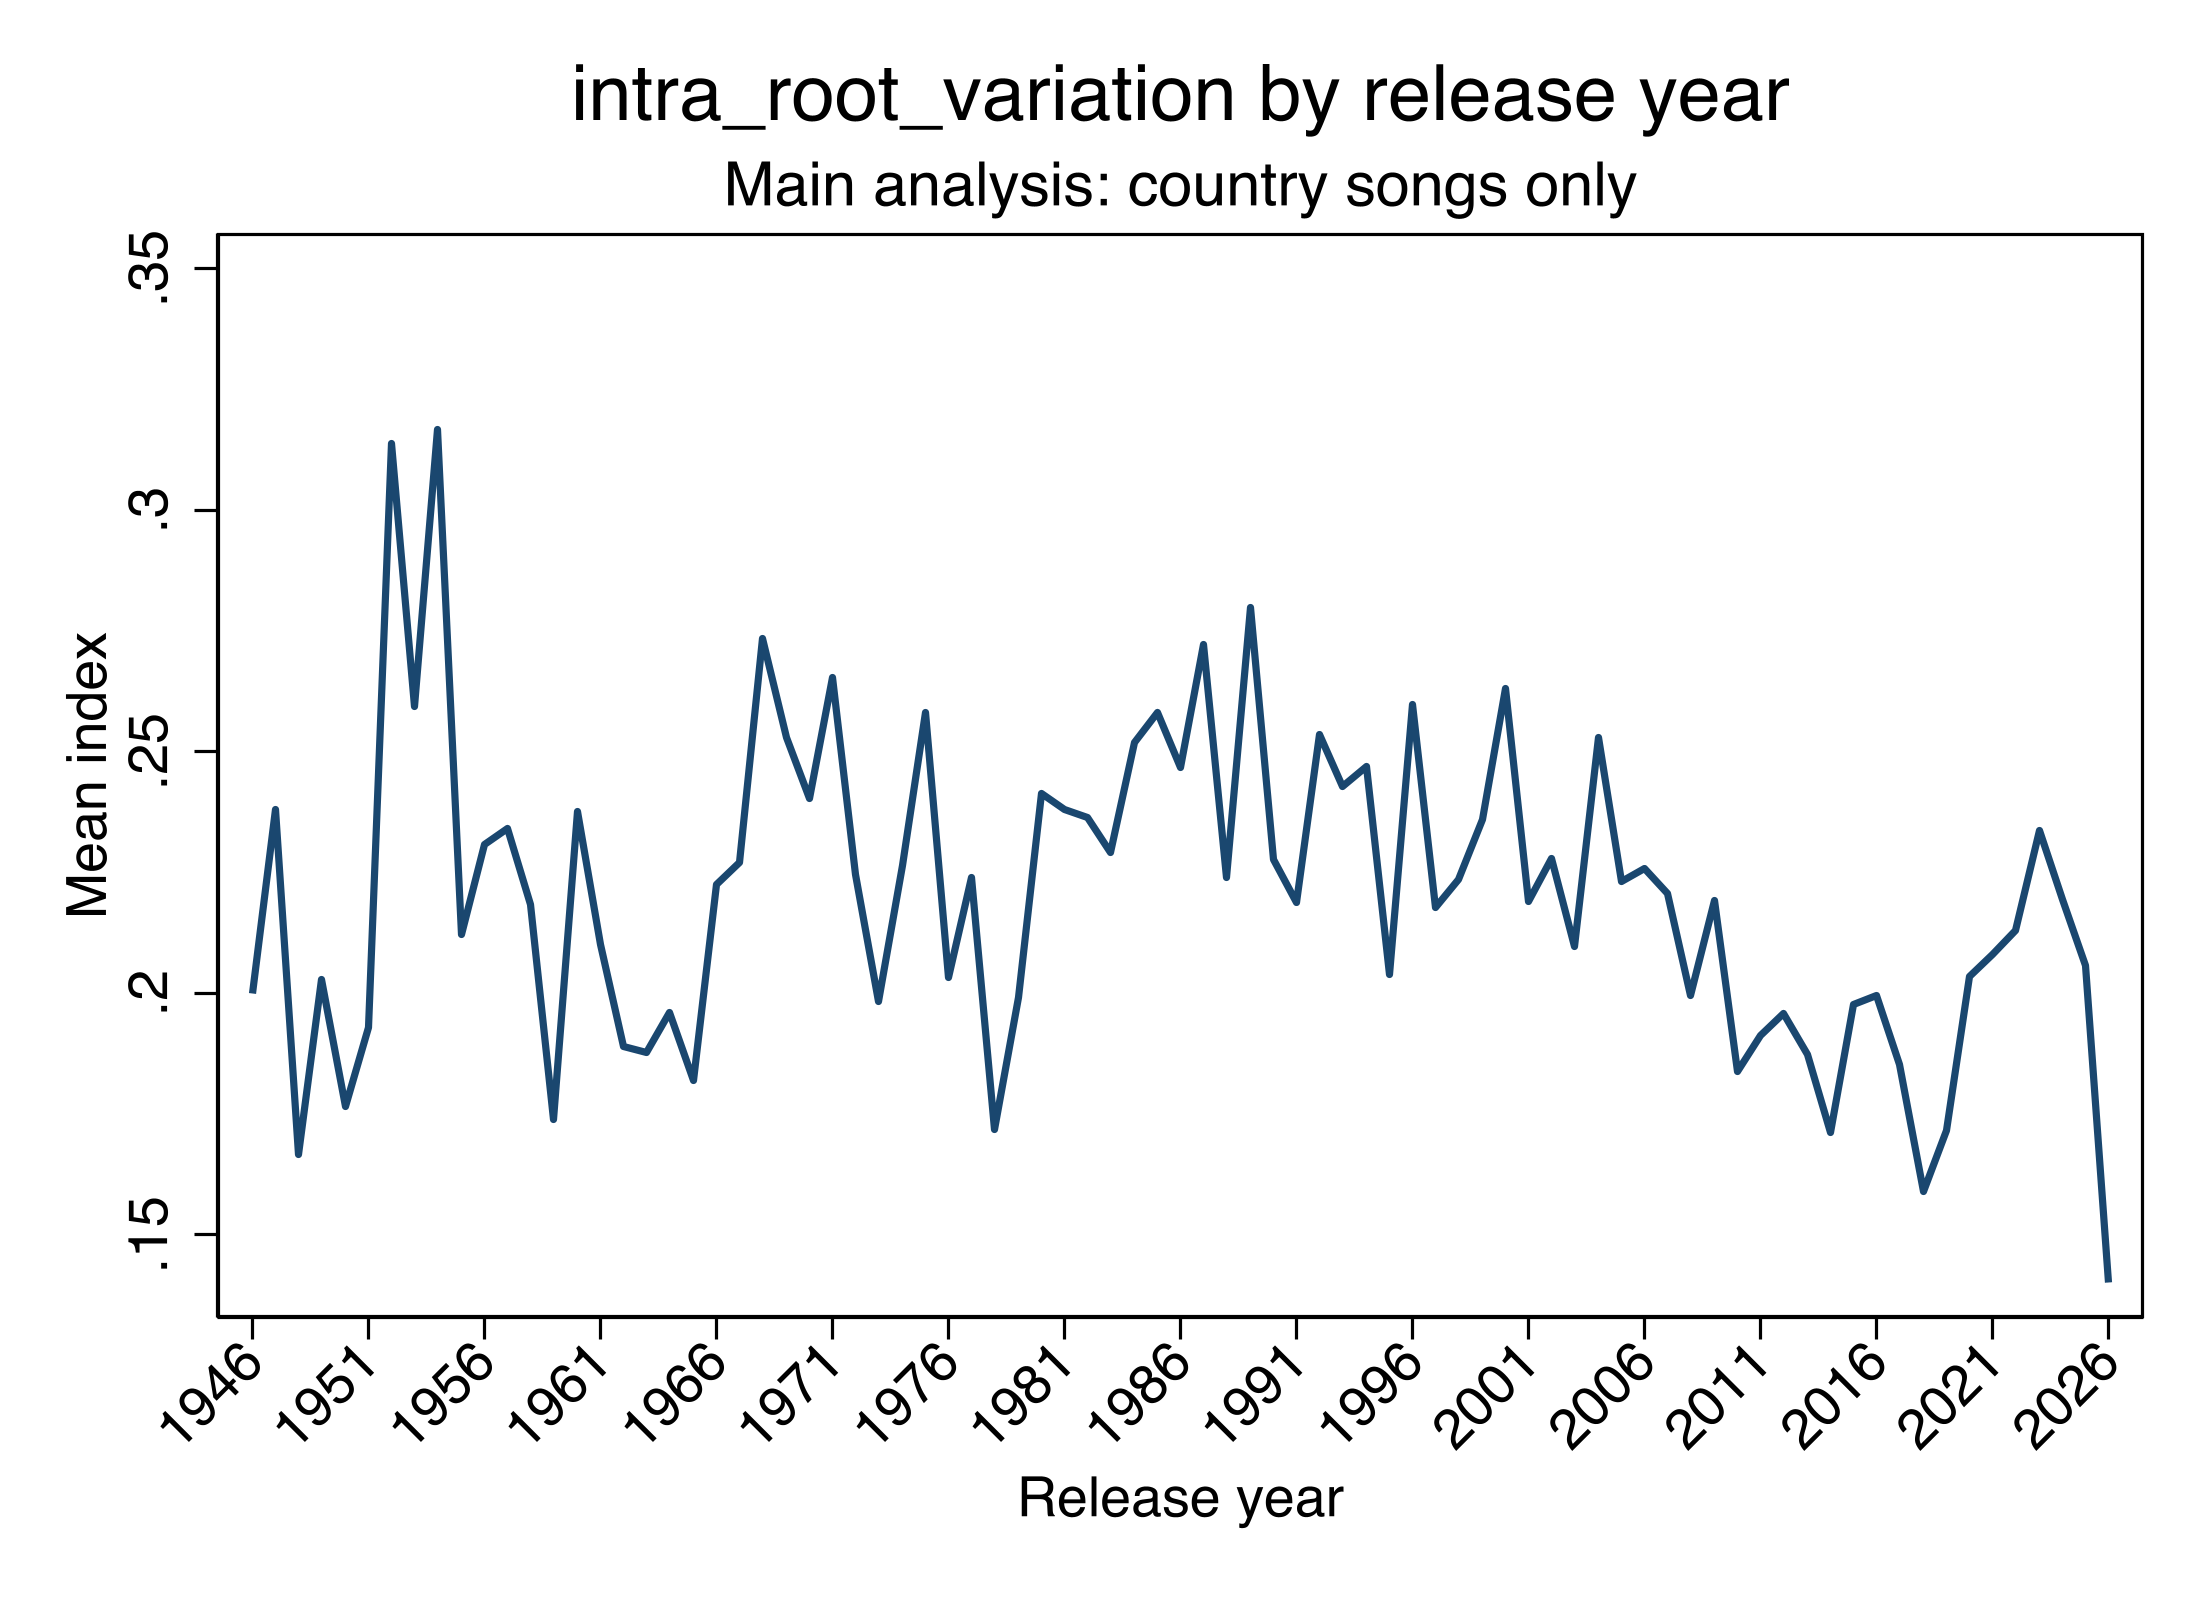
\includegraphics[width=0.88\textwidth]{analysis_outputs/graphs/index_intra_root_variation_by_release_year.png}
\caption{Individual annual trend for intra-root variation}
\end{figure}
Intra-root variation decreases by 0.0064 points per decade ($<0.001$).

\subsection{Harmonic palette: individual annual trend}
\begin{figure}[H]
\centering
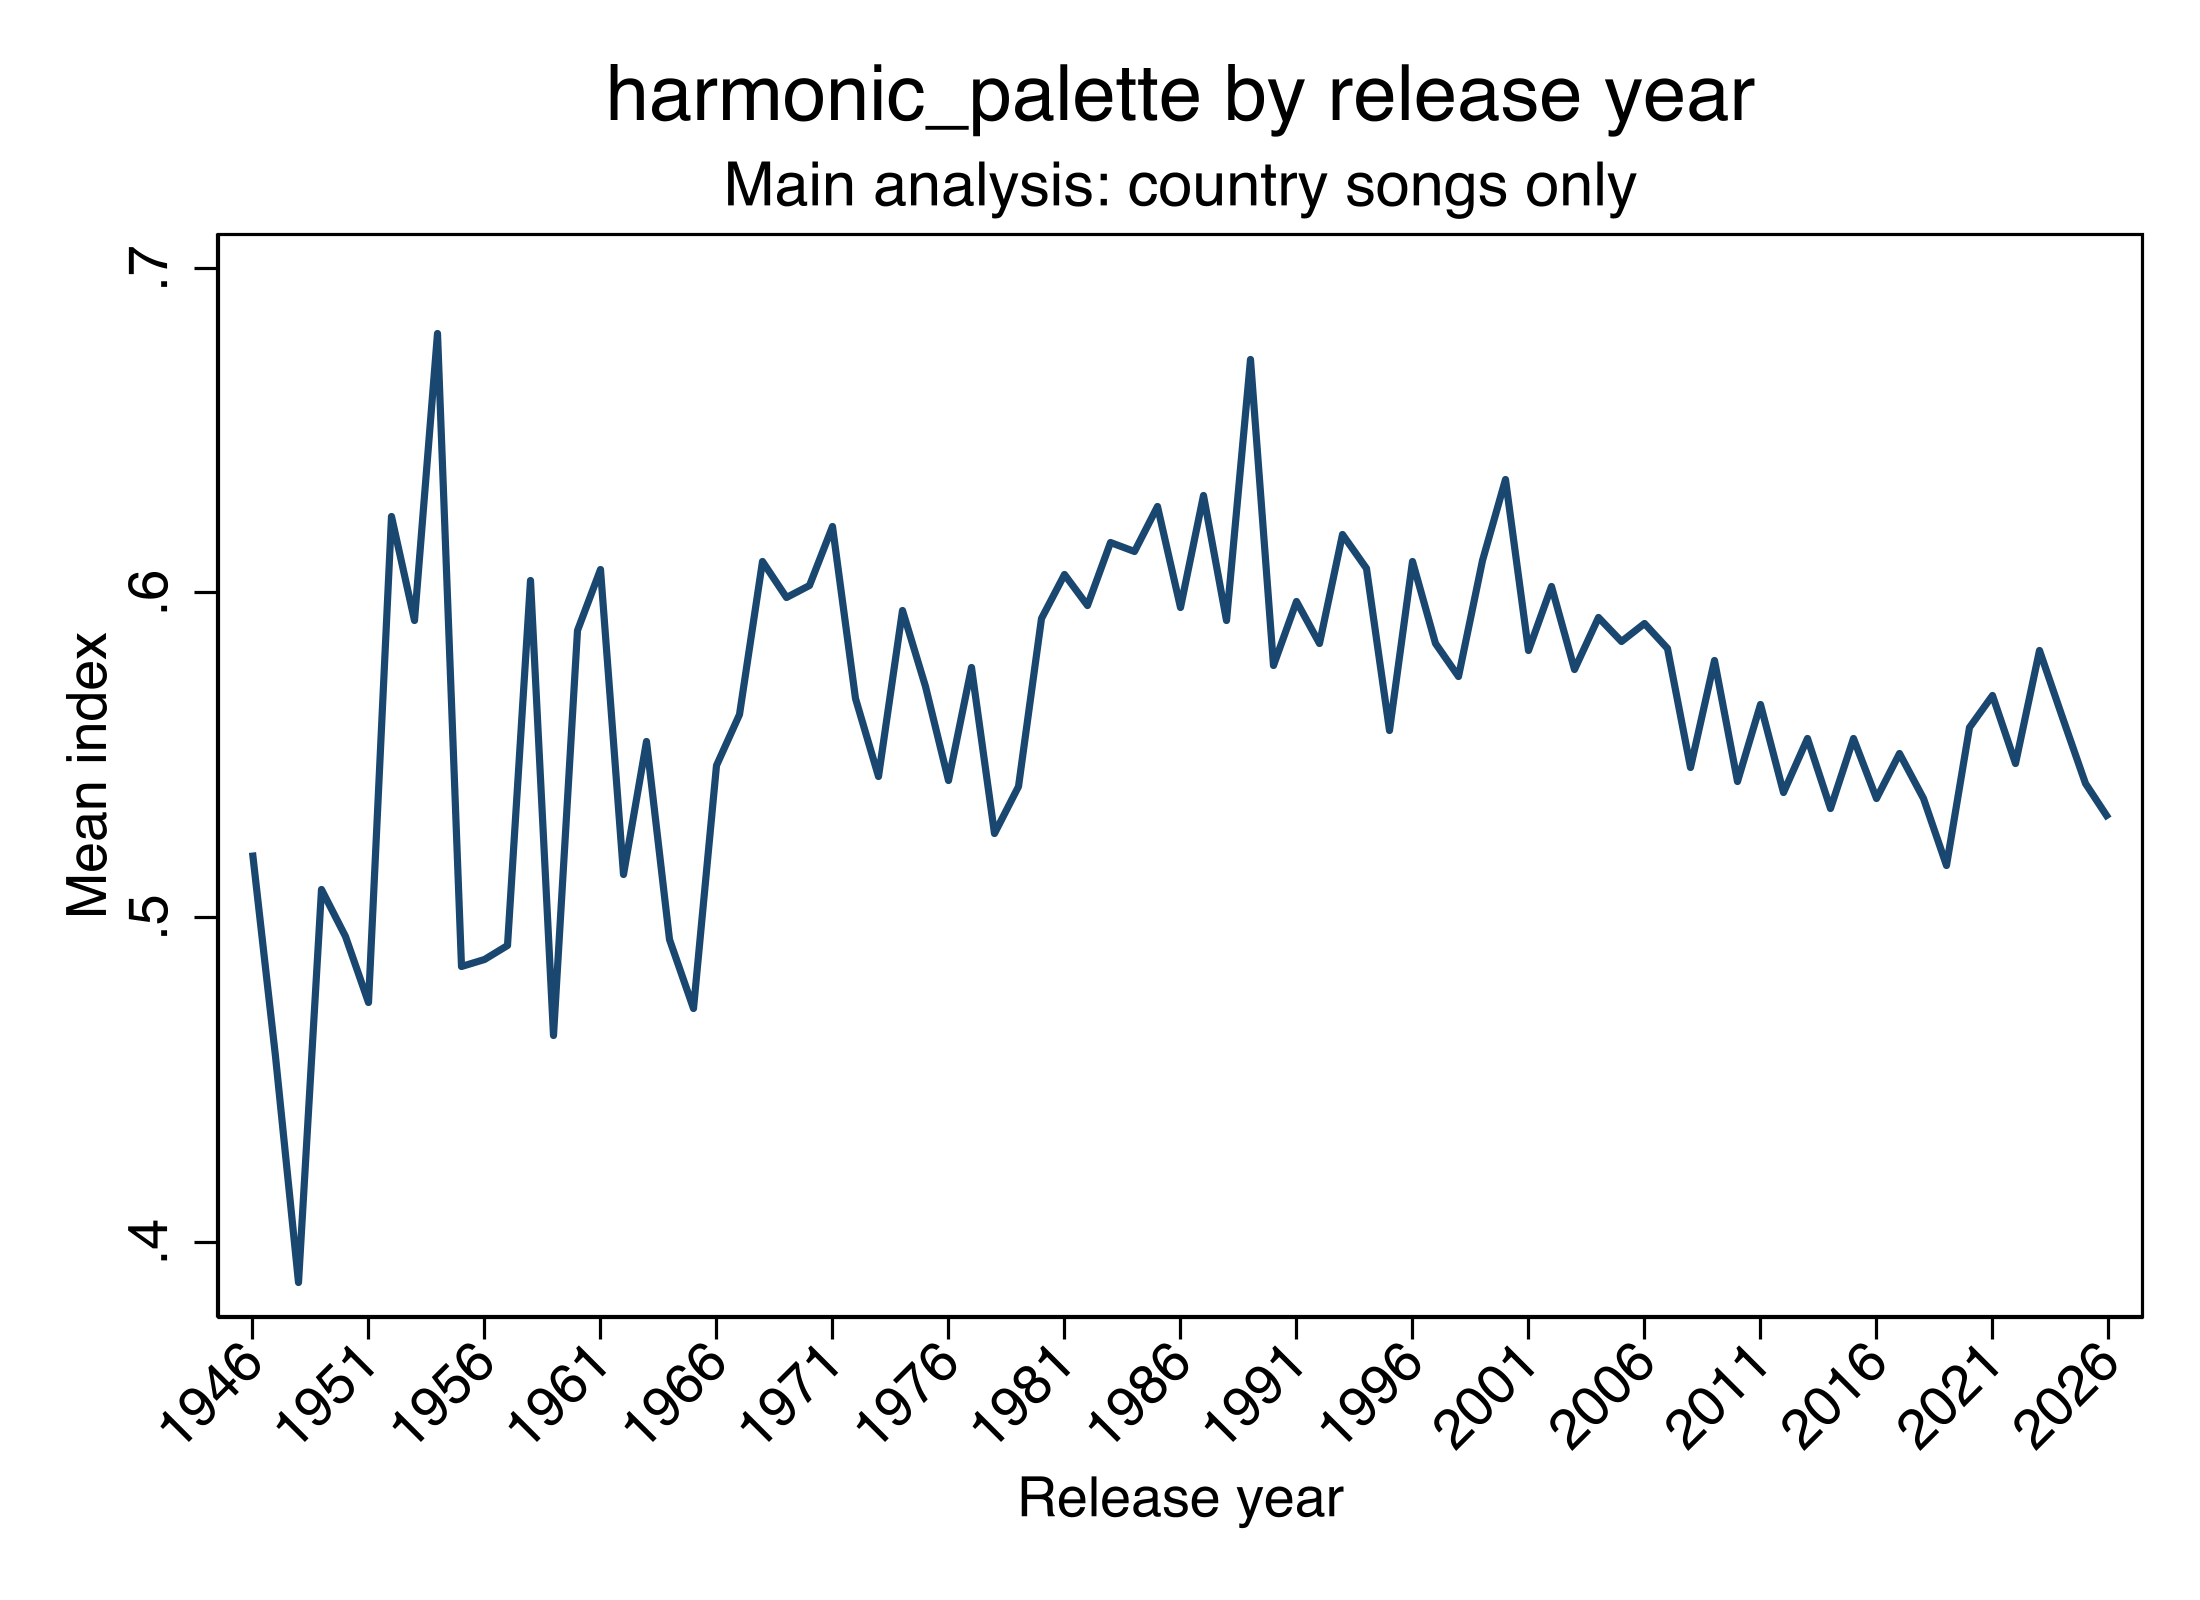
\includegraphics[width=0.88\textwidth]{analysis_outputs/graphs/index_harmonic_palette_by_release_year.png}
\caption{Individual annual trend for harmonic palette}
\end{figure}
Harmonic palette decreases by 0.0045 points per decade ($<0.001$).

\subsection{Loop strength: individual annual trend}
\begin{figure}[H]
\centering
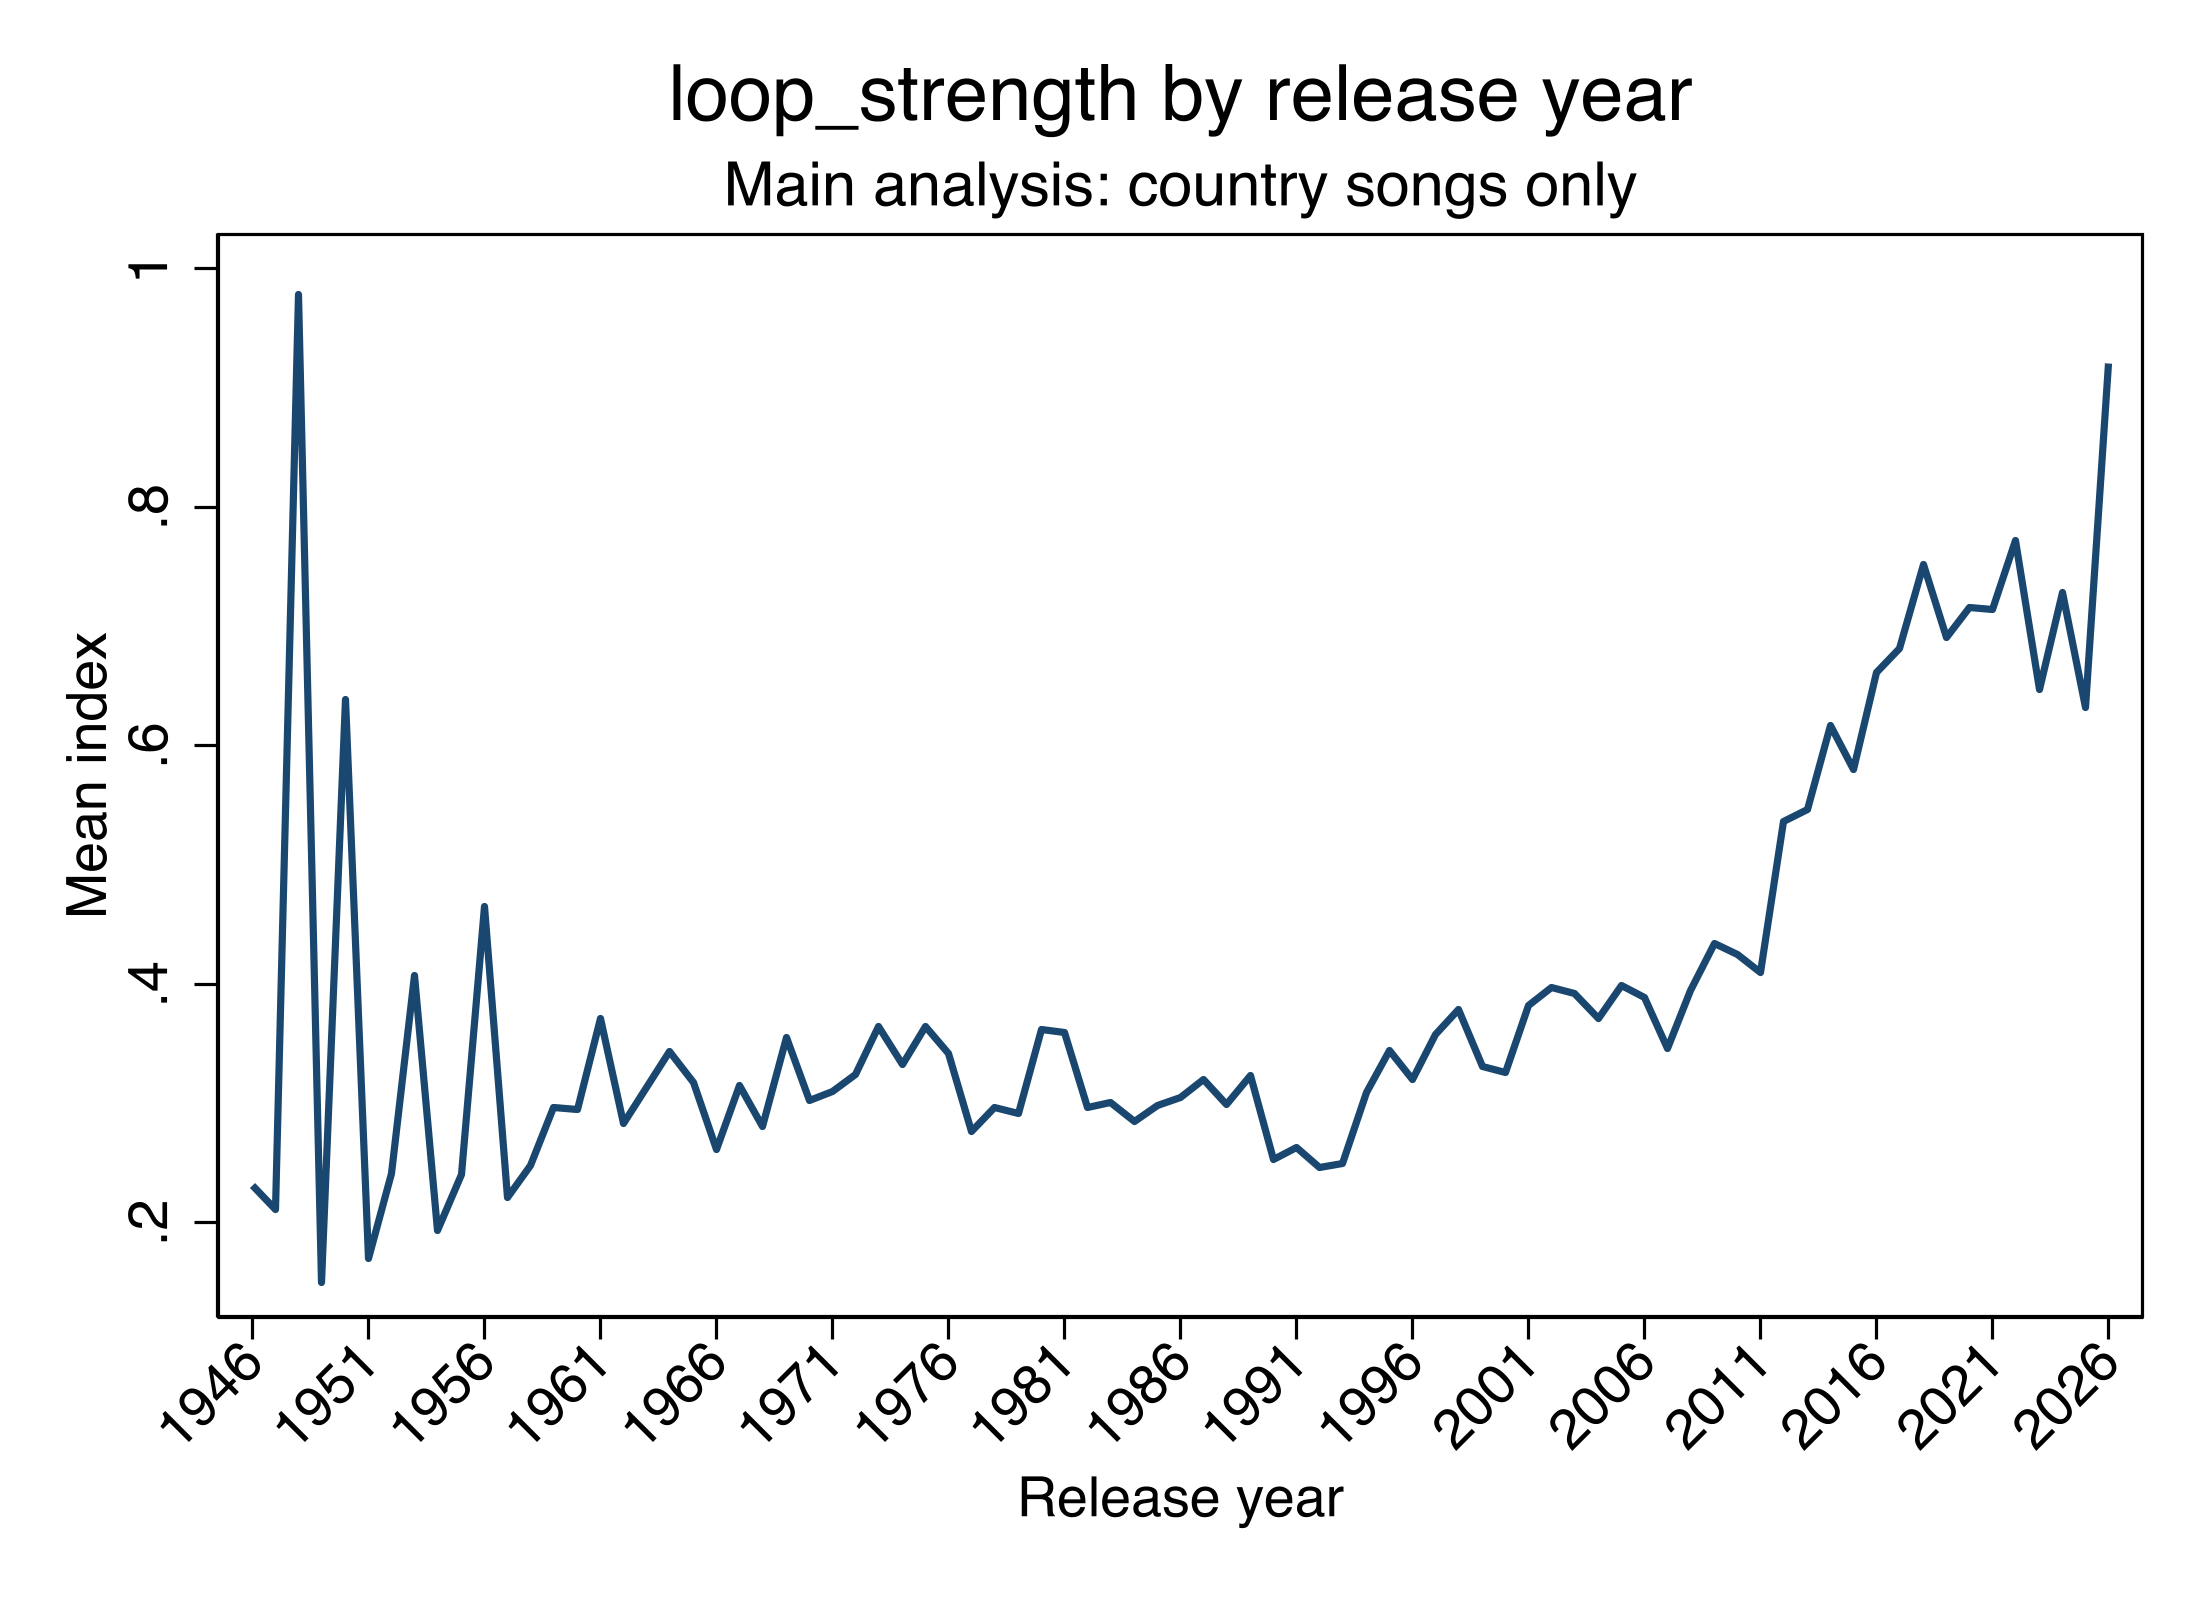
\includegraphics[width=0.88\textwidth]{analysis_outputs/graphs/index_loop_strength_by_release_year.png}
\caption{Individual annual trend for loop strength}
\end{figure}
Loop strength increases by 0.0758 points per decade ($<0.001$).

\subsection{Structure variation: individual annual trend}
\begin{figure}[H]
\centering
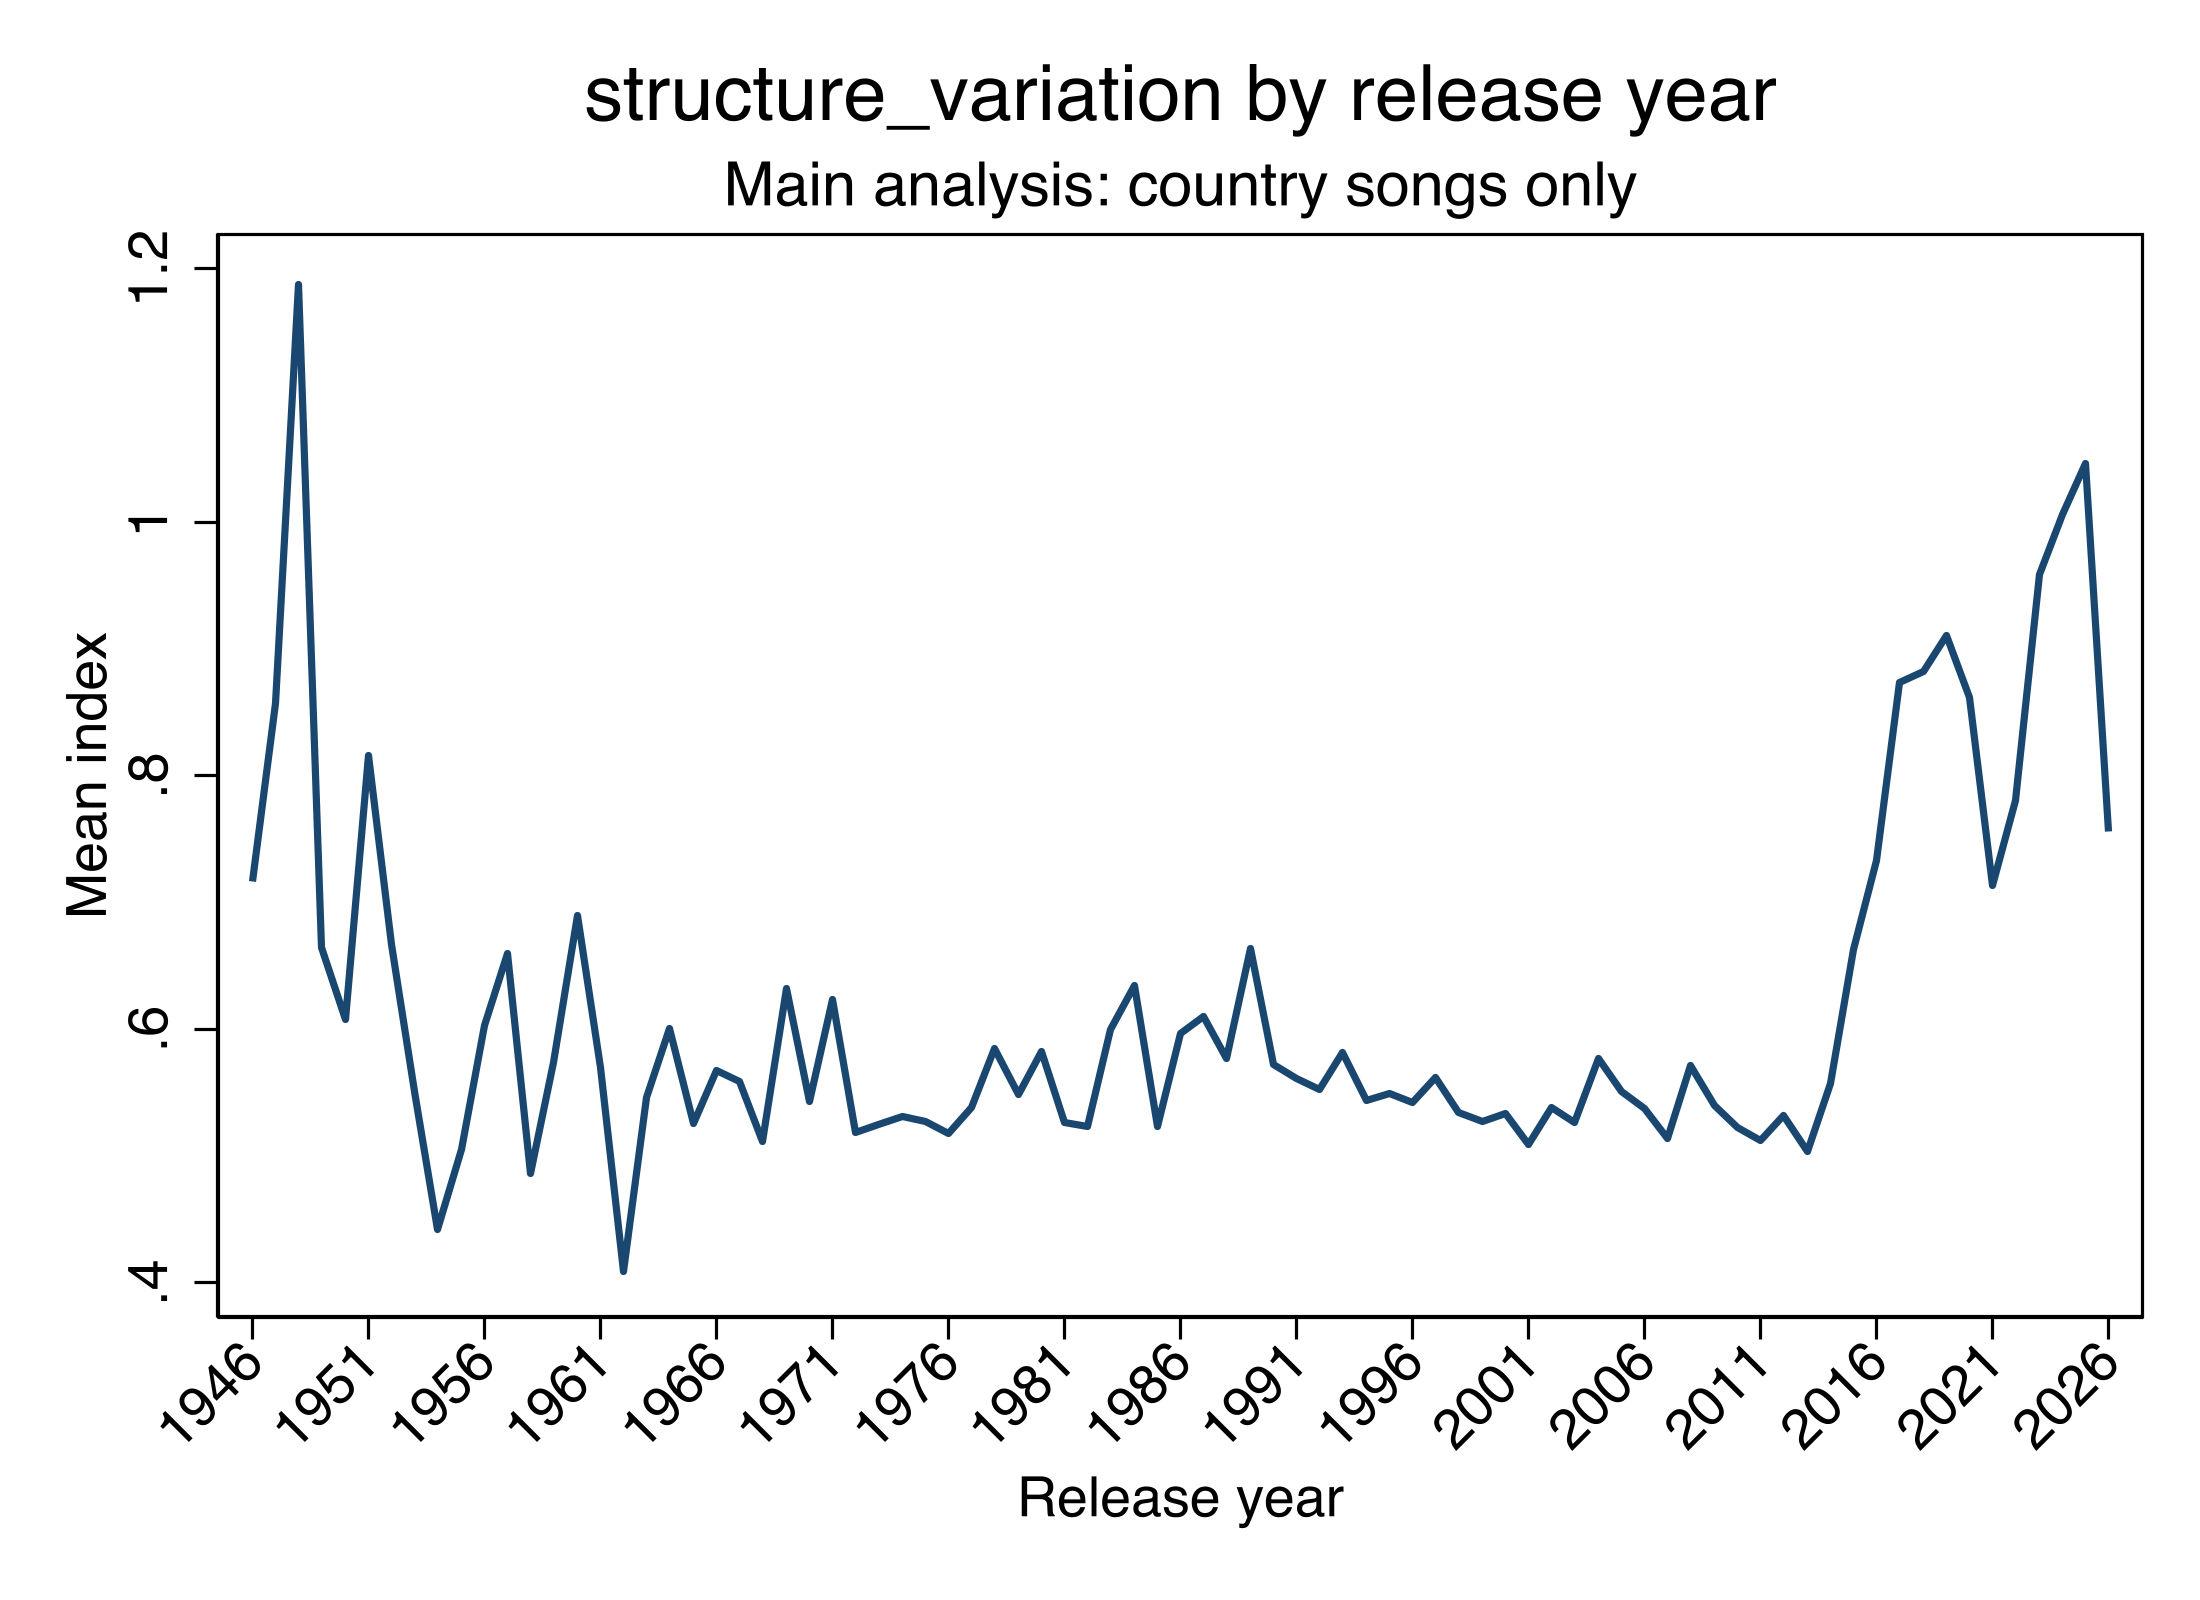
\includegraphics[width=0.88\textwidth]{analysis_outputs/graphs/index_structure_variation_by_release_year.png}
\caption{Individual annual trend for structure variation}
\end{figure}
Structure variation increases by 0.0500 points per decade ($<0.001$).

\subsection{Playability: individual annual trend}
\begin{figure}[H]
\centering
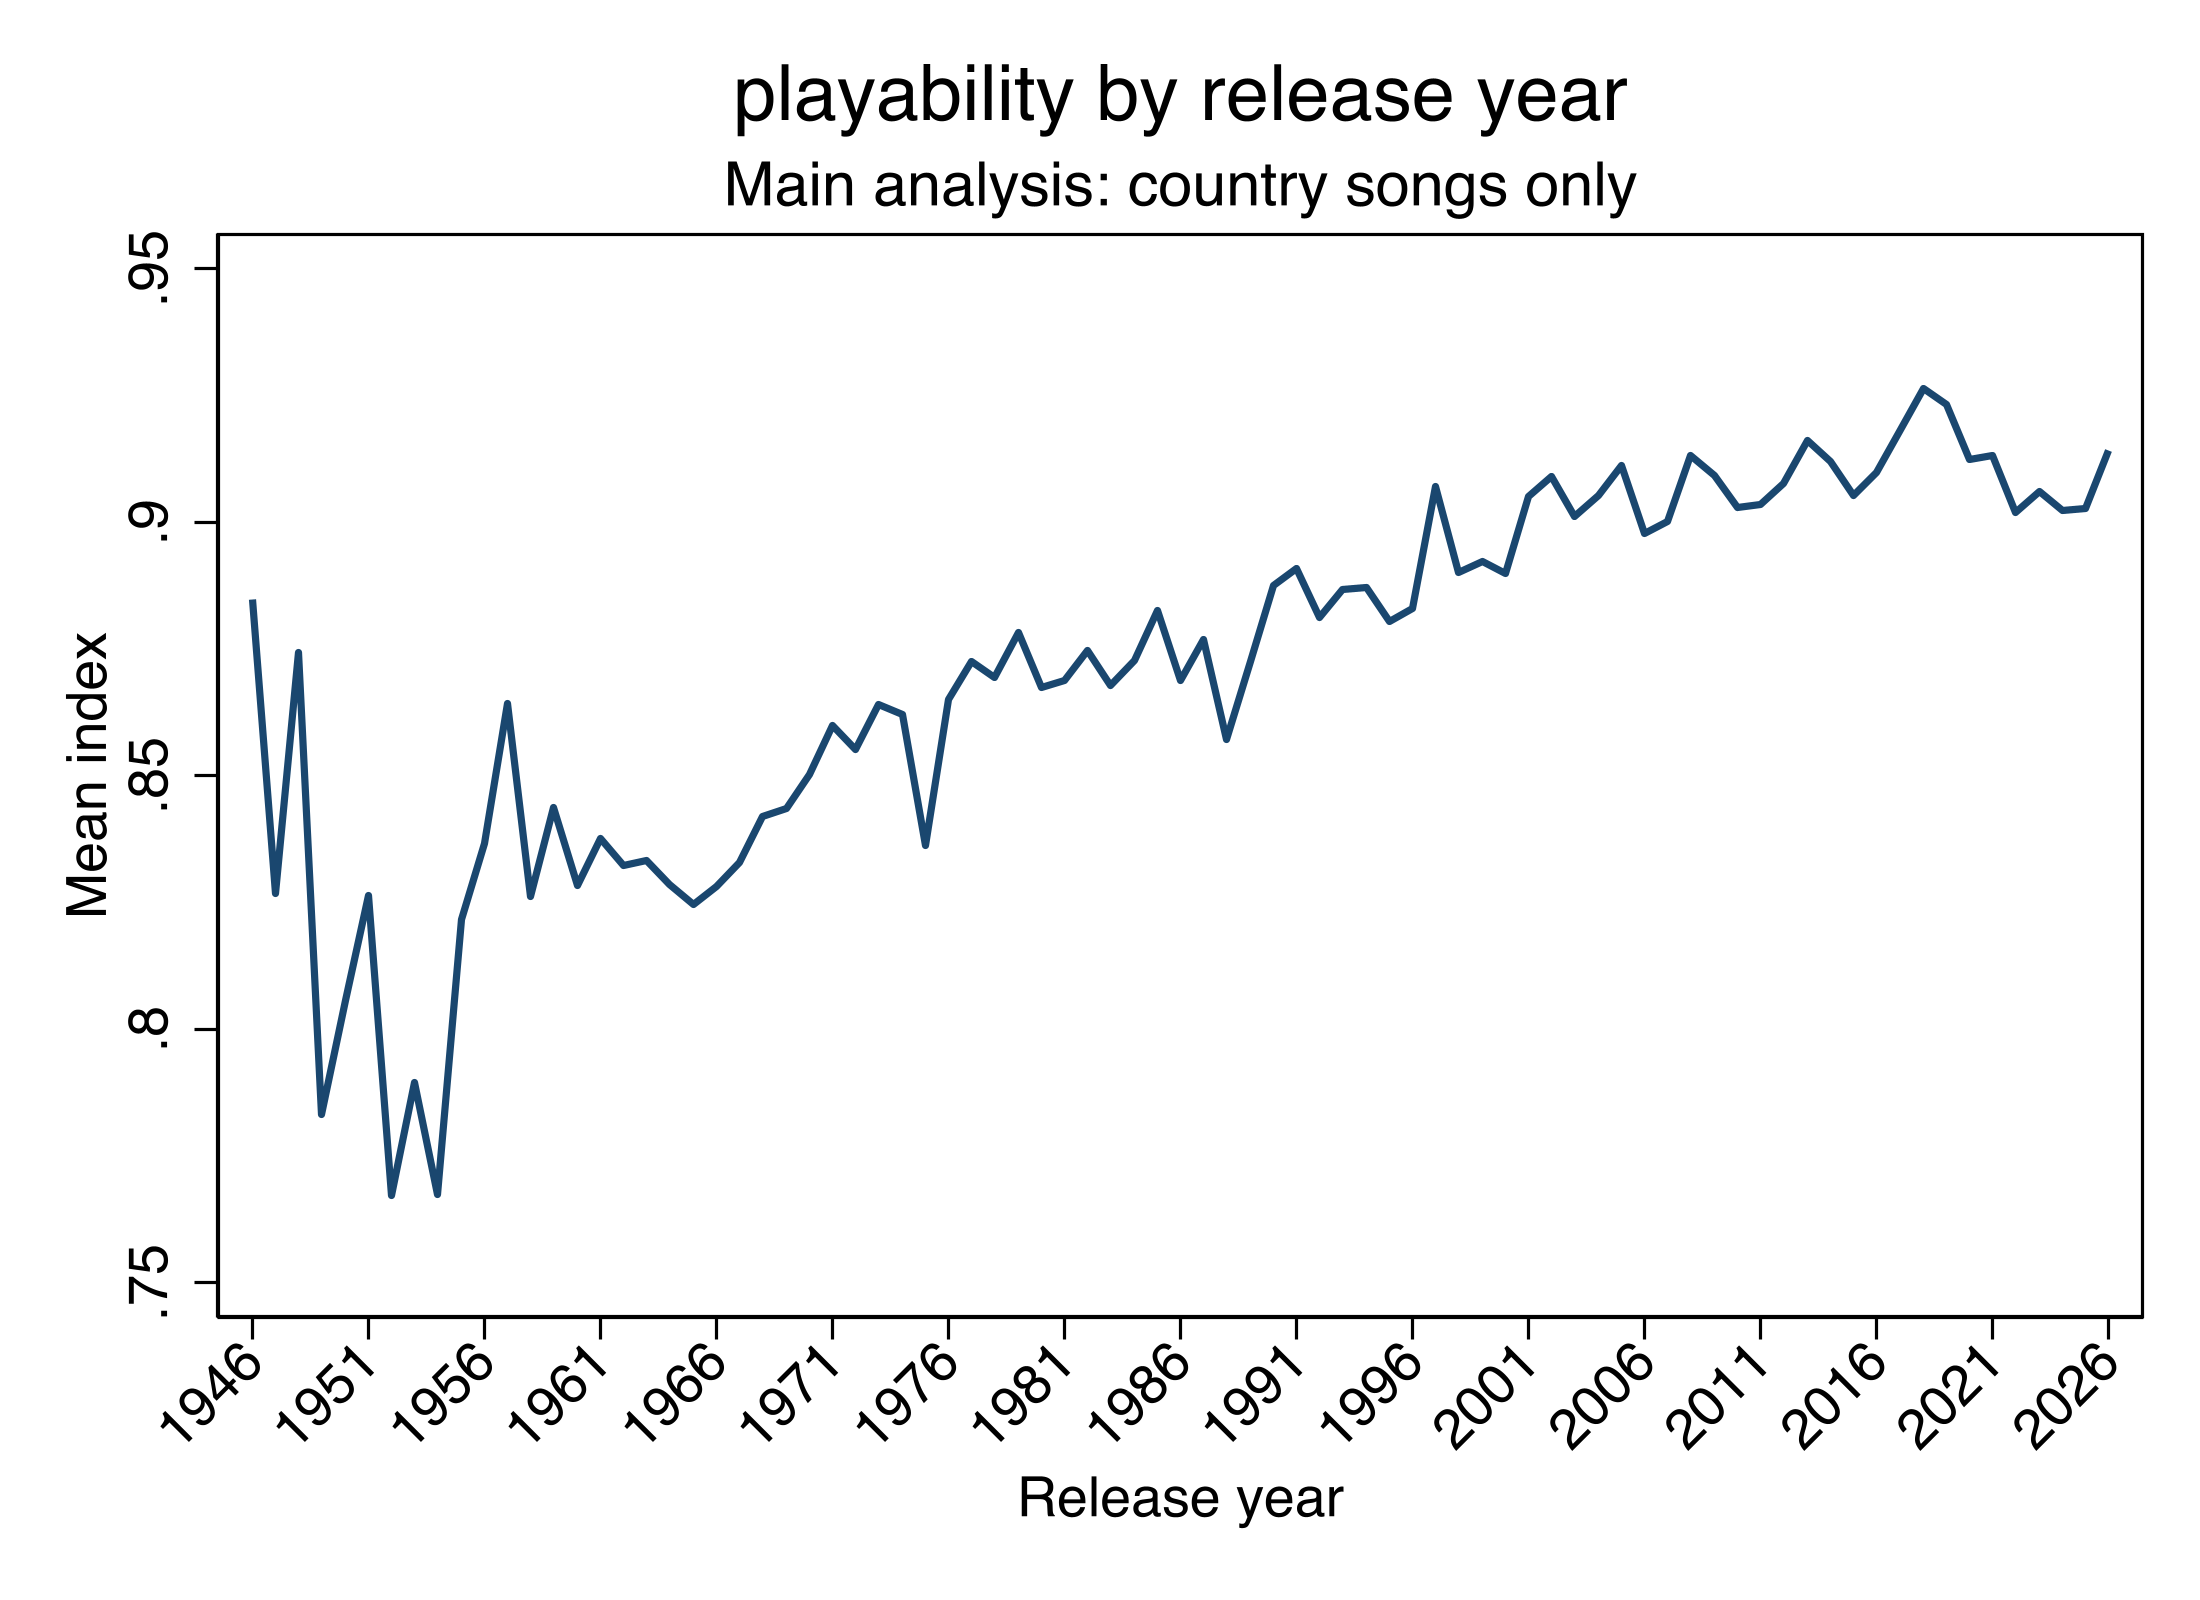
\includegraphics[width=0.88\textwidth]{analysis_outputs/graphs/index_playability_by_release_year.png}
\caption{Individual annual trend for playability}
\end{figure}
Playability increases by 0.0123 points per decade ($<0.001$).

\subsection{Harmonic softness: individual annual trend}
\begin{figure}[H]
\centering
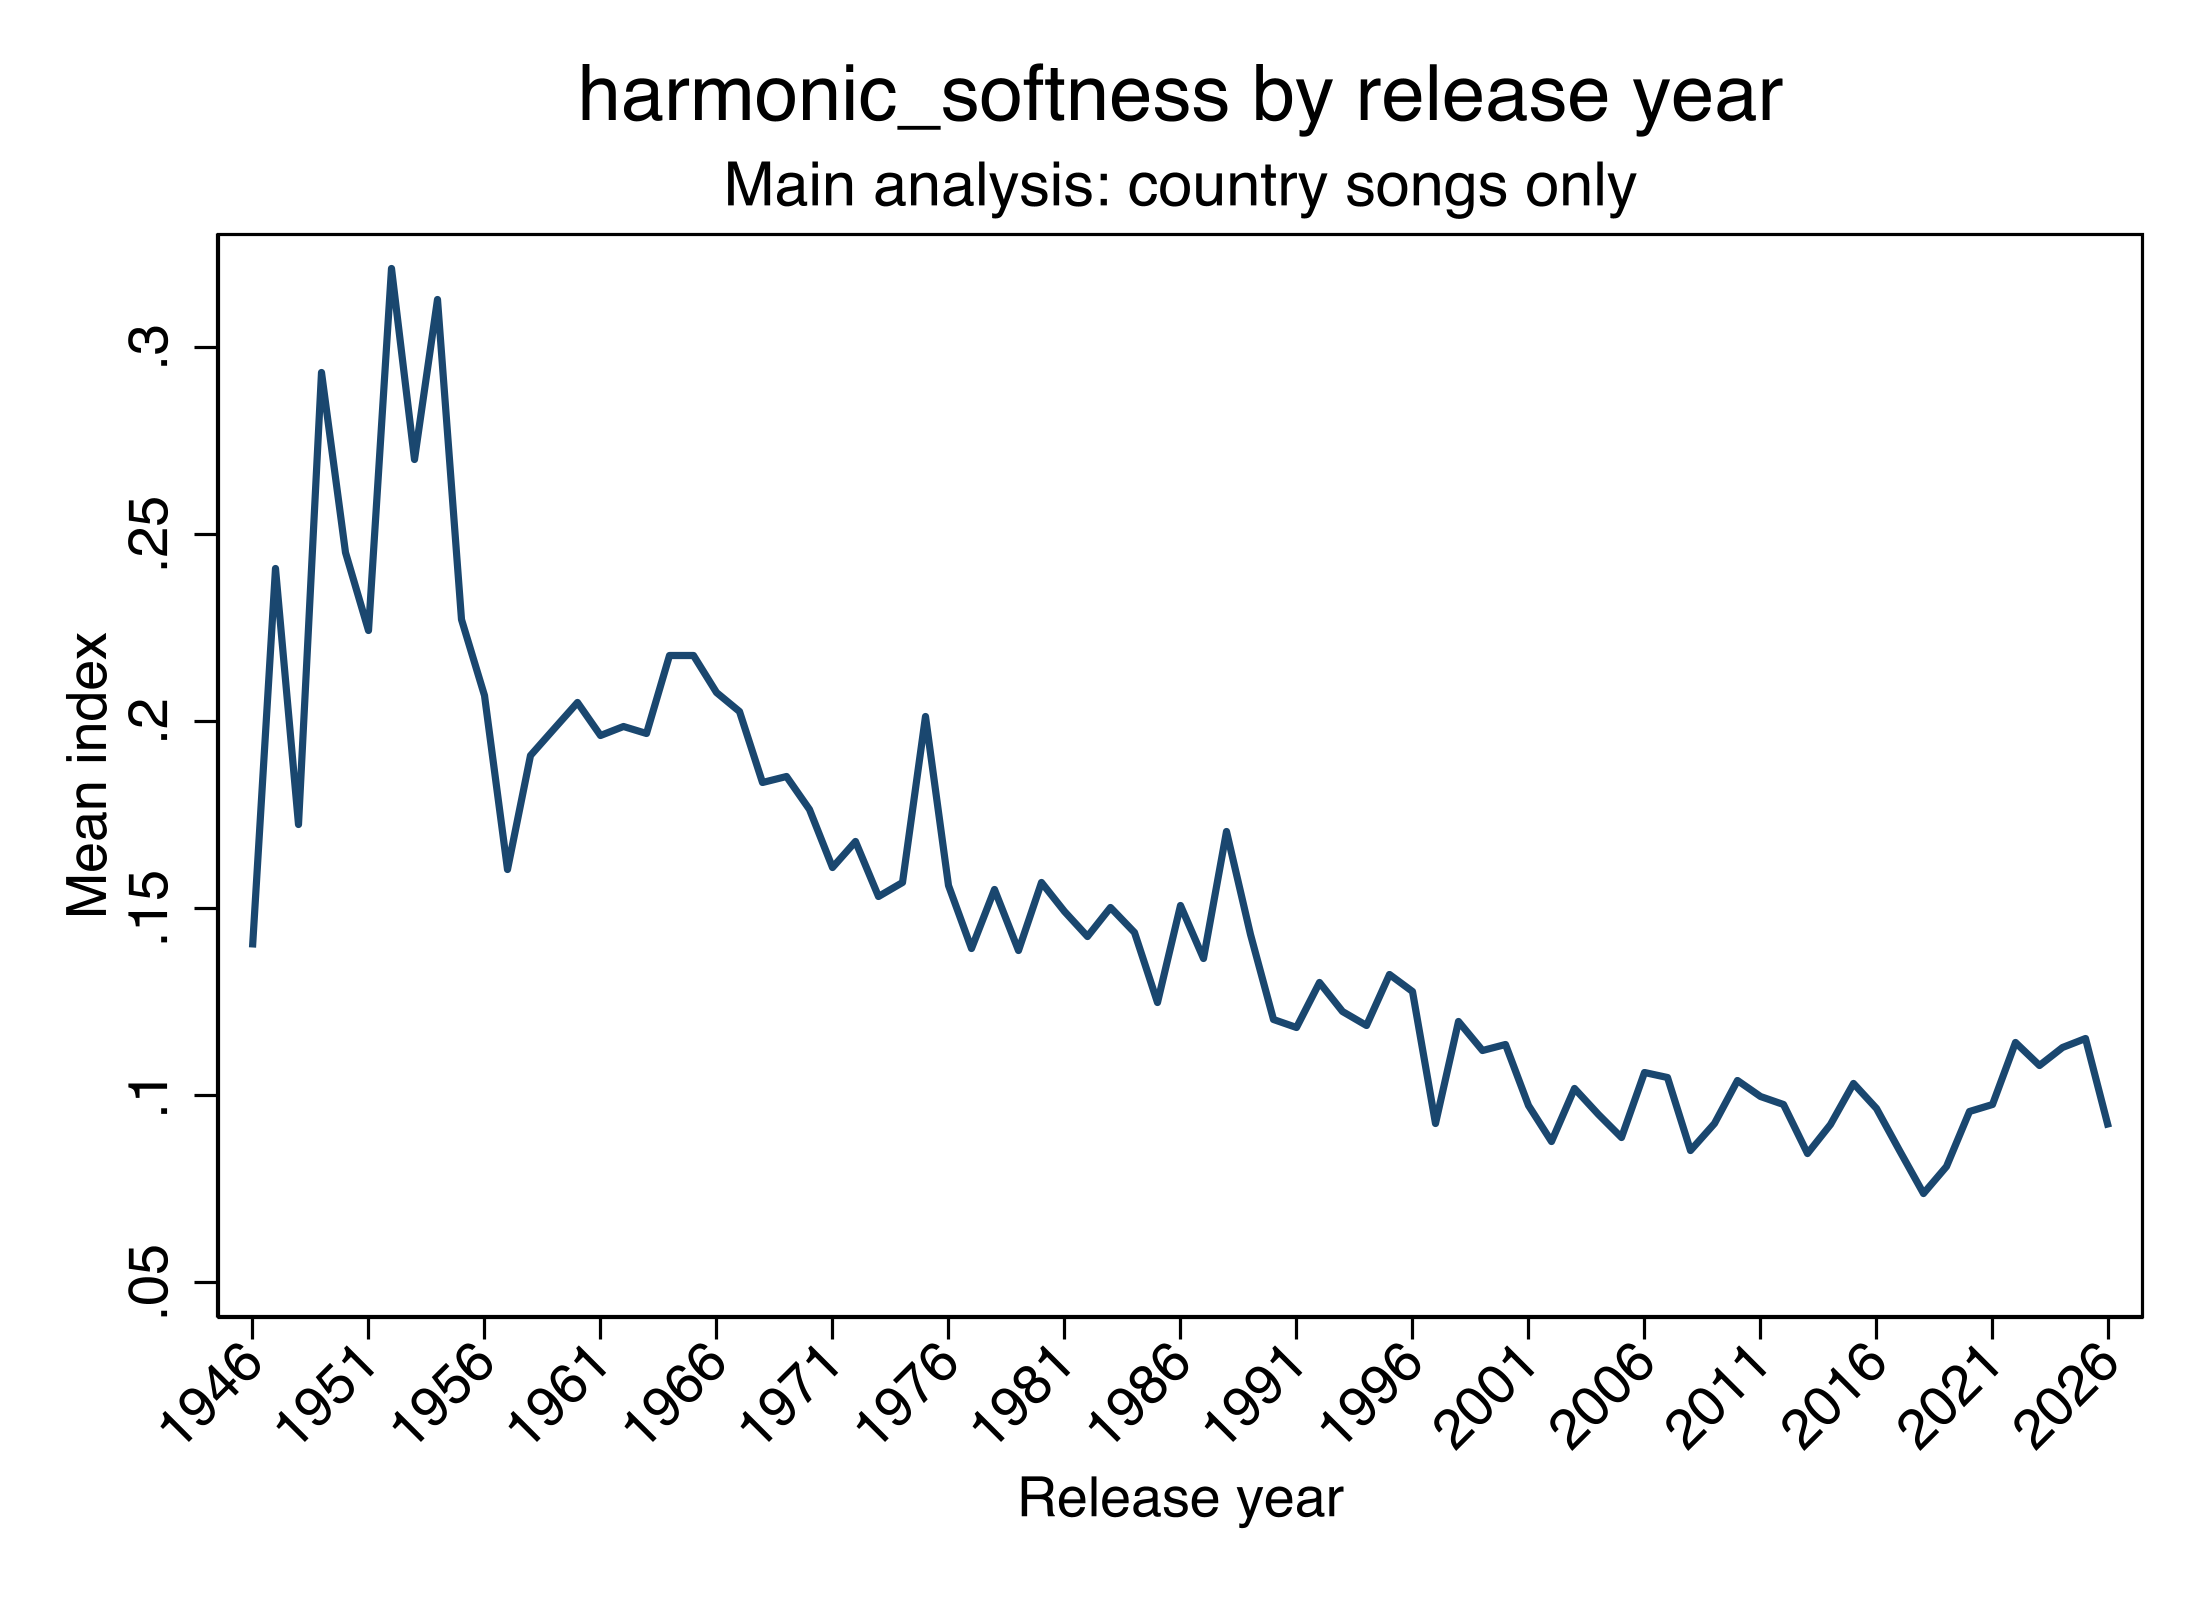
\includegraphics[width=0.88\textwidth]{analysis_outputs/graphs/index_harmonic_softness_by_release_year.png}
\caption{Individual annual trend for harmonic softness}
\end{figure}
Harmonic softness decreases by 0.0160 points per decade ($<0.001$).


\section{Appendix B: Full do-file}
The full Stata script used to create all outputs is reproduced below.

\lstinputlisting{code/eda_country_only_chords_2026_04_08.do}

\end{document}
